\documentclass[11pt]{article}

\usepackage[T1]{fontenc}
\usepackage{lmodern}
\usepackage{amsmath,amssymb,amsthm,mathtools}
\usepackage{graphicx,booktabs,array,enumitem}
\usepackage[margin=1in]{geometry}
\usepackage{microtype}
\usepackage{xcolor}
\usepackage[colorlinks=true,linkcolor=blue!45!black,citecolor=green!35!black,urlcolor=blue!55!black]{hyperref}
\hypersetup{pdftitle={Algebraicity of Kuga--Satake Correspondences for K3 Surfaces},pdfauthor={OpenAI}}
\numberwithin{equation}{section}
\newtheorem{theorem}{Theorem}[section]
\newtheorem{proposition}[theorem]{Proposition}
\newtheorem{lemma}[theorem]{Lemma}
\newtheorem{corollary}[theorem]{Corollary}
\theoremstyle{definition}
\newtheorem{definition}[theorem]{Definition}
\newtheorem{notation}[theorem]{Notation}
\newtheorem{assumption}[theorem]{Assumption}
\theoremstyle{remark}
\newtheorem{remark}[theorem]{Remark}
\newcommand{\Q}{\mathbb Q}
\newcommand{\C}{\mathbb C}
\newcommand{\R}{\mathbb R}
\newcommand{\Z}{\mathbb Z}
\newcommand{\N}{\mathbb N}
\newcommand{\HH}{\operatorname{HH}}
\newcommand{\Ext}{\operatorname{Ext}}
\newcommand{\Hom}{\operatorname{Hom}}
\newcommand{\Perf}{\operatorname{Perf}}
\newcommand{\NS}{\operatorname{NS}}
\newcommand{\CH}{\operatorname{CH}}
\newcommand{\cl}{\operatorname{cl}}
\newcommand{\td}{\operatorname{td}}
\newcommand{\ch}{\operatorname{ch}}
\newcommand{\rk}{\operatorname{rk}}
\newcommand{\id}{\operatorname{id}}
\newcommand{\Spec}{\operatorname{Spec}}
\newcommand{\SO}{\operatorname{SO}}
\newcommand{\End}{\operatorname{End}}
\newcommand{\GL}{\operatorname{GL}}
\newcommand{\Sp}{\operatorname{Sp}}
\newcommand{\KS}{\operatorname{KS}}
\newcommand{\PD}{\operatorname{PD}}
\newcommand{\pt}{\operatorname{pt}}
\newcommand{\Span}{\operatorname{span}}
\newcommand{\articleid}[1]{\begingroup\ttfamily\small\def\-{-\allowbreak}#1\endgroup}
\setlength{\emergencystretch}{2em}

\title{Algebraicity of Kuga--Satake Correspondences\\for K3 Surfaces}
\author{OpenAI}
\date{October 3, 2026}
\begin{document}
\maketitle
\begin{abstract}
We prove that the Kuga--Satake correspondence is algebraic for every smooth projective complex K3 surface. More precisely, the prescribed embedding of its transcendental cohomology into the cohomology of its Kuga--Satake abelian variety is induced by a rational algebraic cycle, with the fixed normalization and full even-Clifford target. The result also holds for isogenous Kuga--Satake models with the transported embedding.
\end{abstract}
\tableofcontents

\section{Introduction}
\label{sec:introduction}

The Kuga--Satake construction places a polarized Hodge structure of
K3 type inside the tensor square of a weight-one Hodge structure.
For a projective K3 surface, this realizes its transcendental
cohomology inside the cohomology of an abelian variety.  The
algebraicity question asks whether this Hodge-theoretic relation is
induced by an algebraic cycle.  It is a particular case of the Hodge
conjecture, with a specified tensor to be realized.

\subsection{The correspondence to be realized}

Let $S$ be a smooth projective complex K3 surface.  Write
\[
 T(S)=\NS(S)_\Q^{\perp}\subset H^2(S,\Q),
\]
where orthogonality is with respect to cup product.  Equip this
transcendental Hodge structure with the polarization used in the
Kuga--Satake construction.  Fix the standard construction data and
let $A_S=\KS(T(S))$ denote the full even-Clifford Kuga--Satake
abelian variety, with its fixed rational polarization.  If
$W_S=H^1(A_S,\Q)$, the construction gives an embedding
\[
             T(S)(1)\lhook\joinrel\longrightarrow\End(W_S).
\]
The polarization identifies $W_S^\vee$ with $W_S(1)$, so untwisting
and using the K\"unneth inclusion gives a specified Hodge embedding
\begin{equation}
 \kappa_S:T(S)\lhook\joinrel\longrightarrow
       W_S\otimes W_S\lhook\joinrel\longrightarrow
       H^2(A_S\times A_S,\Q).
 \label{eq:prescribed-ks-map}
\end{equation}
The fixed data in this definition matter: the theorem concerns this
map itself, including its normalization and its full Clifford target.

For smooth projective varieties $S$ and $Z$, with $S$ a surface, a
class $\Gamma\in\CH^2(S\times Z)_\Q$ acts on degree-two cohomology
by
\[
 \Gamma_*(x)=(p_Z)_*\bigl(\cl(\Gamma)\smile p_S^*x\bigr).
\]
Here $\CH^2$ denotes codimension-two algebraic cycles modulo rational
equivalence, with rational coefficients, and $\cl$ is the Betti cycle
class.  Integration over $S$ reduces degree by four, so this formula
does take values in $H^2(Z,\Q)$.

\begin{theorem}
\label{thm:main}
For every smooth projective complex K3 surface $S$, and for every
fixed set of standard Kuga--Satake construction data as above, there
is a cycle
\[
             \Gamma_S\in\CH^2(S\times A_S\times A_S)_\Q
\]
such that $\Gamma_{S*}|_{T(S)}=\kappa_S$.
The same assertion holds for an isogenous Kuga--Satake model when
the prescribed map is transported by the corresponding rational
Hodge isomorphism.
\end{theorem}


\subsection{Historical context and related work}

Kuga and Satake introduced their construction in 1967
\cite{History:KugaSatake}.  It associates an abelian variety to
polarized K3 cohomology through the spin representation of its
Clifford algebra.  This association allows questions about
weight-two cohomology to be studied through weight-one cohomology,
where abelian varieties provide geometric tools.  Deligne used
the construction in his proof of the Weil conjecture for K3
surfaces \cite{History:DeligneK3}.  His work also establishes the
absolute-Hodge character of the Kuga--Satake correspondence;
see \cite{History:DeligneK3,History:DeligneHodge}.
Andr\'e subsequently proved that this correspondence is motivated
\cite[Section~7]{History:Andre}.  These results give the tensor
strong functorial and arithmetic properties.  Its realization by
an algebraic cycle is the further assertion addressed here.

Geometric realizations in special cases have long played an
important role.  Morrison analyzed the Kuga--Satake variety
attached to an abelian surface \cite{History:Morrison}.
Paranjape constructed the relevant algebraic correspondence for
K3 surfaces obtained by resolving double covers of the plane
branched along six lines in general position
\cite{History:Paranjape}.  This gives a four-dimensional family
whose general member has Picard number sixteen.  Van Geemen
developed the Clifford-algebra and Hodge-theoretic description
in detail and explained formulations of the algebraicity problem
using surface covers and products of holomorphic one-forms
\cite[Sections~10--11]{History:VanGeemen}.  His cyclic quartic
examples provide another geometric realization
\cite[Example~11.3]{History:VanGeemen}.  These formulations
motivate our search for a nonzero correspondence; recovery of
the prescribed tensor is handled by the reduction stated below.

A more recent source of examples comes from hyperk\"ahler
varieties of generalized Kummer type.  O'Grady related their
Kuga--Satake varieties to intermediate Jacobians
\cite{History:OGrady}.  Combining this description with
Markman's results on algebraic cycles and Abel--Jacobi maps
\cite{History:MarkmanKummer}, Voisin proved algebraicity of the
Kuga--Satake correspondence for projective varieties of generalized
Kummer type of dimension at least four
\cite[Theorem~0.5]{History:VoisinKummer}.
Floccari then used associated K3 surfaces to obtain algebraicity
for further families of K3 surfaces
\cite{History:Floccari2024,History:Floccari2026}.  In particular,
\cite[Theorem~5.11]{History:Floccari2026} applies whenever
$T(S)$ admits an isometric embedding into
$U_\Q^{\oplus 3}\oplus\langle-m\rangle_\Q$ for a positive
integer $m$, where $U$ is the hyperbolic plane.  That result
also proves the Hodge conjecture for every power of these K3
surfaces.  The hyper-Kummer construction of Floccari and Fu
proves that the Chow motives in certain families with generic
Picard number sixteen are of abelian type
\cite{History:FloccariFu}.

Low Picard number also occurs in this special-family literature.
Bolognesi and Laterveer study two nine-dimensional families of K3
surfaces with generic Picard number two, distinguished by a
non-symplectic automorphism of order three fixing a curve.  They
state Kuga--Satake algebraicity results for these families
\cite[Theorem~4.4, Propositions~6.2 and~6.4]{History:BolognesiLaterveer}.
Theorem~\ref{thm:main} addresses this algebraicity problem for
every projective K3 surface, in the fixed formulation stated
above.

Two further strands of work enter the proof.  Buskin proved that
rational Hodge isometries between projective K3 surfaces are
algebraic \cite{Deformation:Buskin}.  We use this result to
transfer algebraic correspondences between suitable K3 Hodge
structures.  For the deformation step, the relevant ancestry
is the semiregularity theory of Buchweitz--Flenner and its
extension to perfect complexes by Pridham
\cite{Deformation:BF2003,Deformation:Pridham}.
Markman's secant-sheaf approach combines spinor geometry,
Fourier--Mukai transforms, and semiregularity to construct
algebraic Weil classes, including those on split abelian
sixfolds \cite{History:MarkmanSecant,History:MarkmanSurvey}.
Our proof likewise constructs an object that can deform while
its characteristic classes remain of Hodge type.  The
specific task is to obtain such an object with enough
deformation directions to cover polarized K3 moduli.
The fixed mirror-symmetry theorems and the immersed-Lagrangian
construction described below supply it.


\subsection{The reduction to a nonzero correspondence}

The proof uses the following reduction from the companion manuscript
\cite{R}.  A polarization below is ample and primitive in the
integral K3 lattice.  A property holds at a very general point if it
holds outside a countable union of proper closed algebraic subsets
of the relevant moduli space.

\begin{theorem}[Reduction to very general polarized K3 surfaces]
\label{thm:reduction}
Assume that for every positive integer $d$, a very general
primitively polarized complex K3 surface $(S,h)$ with $h^2=2d$
admits an abelian variety $B_S$ and a cycle
\[
       Z_S\in\CH^2(S\times B_S)_\Q
\]
whose action is nonzero on $h^\perp\subset H^2(S,\Q)$.
Then Theorem~\ref{thm:main} holds.
\end{theorem}

This is the combination of Theorems~1.1 and~1.2 and
Corollary~1.3 of~\cite{R}.  Its content has two parts.  At a very
general polarized K3 surface, the full orthogonal Hodge group and
the spin representation recover the prescribed full Kuga--Satake
tensor from any nonzero algebraic correspondence of the displayed
kind.  Algebraic correspondences then specialize through the
polarized moduli space.  The reduction includes comparison with
the stipulated construction data at special fibers.  We shall use
the reduction in this precise form; the main task of the present
paper is to construct its nonzero algebraic input.

\subsection{The proof mechanism}

Fix a positive integer $d$.  We begin with a K3 surface $S$ of
Picard number nineteen and an abelian variety $B=E^g$, where $E$ is
a non-CM elliptic curve and $g=512$.  These varieties are mirrors
of a symplectic quartic $P$ and a standard symplectic torus $Y$.
Only mirror symmetry at these fixed varieties is used.  The
auxiliary dimension $512$ permits a rational Clifford
representation with eighteen specified symmetric generators; its
size is not a dimension assertion about the Kuga--Satake variety
in Theorem~\ref{thm:main}.

Choose an ample rational class $h$ on the starting K3 with square
$2d$.  A rational class is sufficient at this stage; the relation
between its primitive integral ray and degree $2d$ will be handled
at the end.  Put
\[
             M=P\times Y,\qquad n=g+2,\qquad
             D_{\mathrm{tot}}=22+\binom{2g}{2}.
\]
The proof constructs a perfect complex $\mathcal E$ on $S\times B$
with two complementary properties.

First, topology gives the upper bound
\begin{equation}
             \dim\Ext^2(\mathcal E,\mathcal E)
                    \le D_{\mathrm{tot}}-19.
 \label{eq:intro-upper}
\end{equation}
We construct a rational class $\alpha\in H^n(M,\Q)$ for which
cup product $H^2(M,\Q)\to H^{n+2}(M,\Q)$ has a prescribed
nineteen-dimensional kernel.  A torus bundle and surgery realize
a multiple of its Poincar\'e dual by an immersed Lagrangian
$L\to M$ with
\[
       b_2(L)=D_{\mathrm{tot}}-19,
       \qquad H_{n-2}(L,\Q)\longrightarrow H_{n-2}(M,\Q)
       \text{ injective}.
\]
The immersion has only odd-degree double-point sectors.  The
homological injection detects its Floer obstruction, and the
absence of degree-two double-point generators bounds its second
self-Floer group by $b_2(L)$.  A representability and trace-pairing
argument makes $\mathcal E$ a direct summand of the resulting
Floer object, proving \eqref{eq:intro-upper}.

Second, intersection numbers prescribe the component of the Mukai
vector $v(\mathcal E)=\ch(\mathcal E)\sqrt{\td}$ with algebraic
K3 coefficients.  Eighteen anticommuting matrices control this
component.  The Hochschild cap action factors through
\[
 \HH^2(S\times B)\longrightarrow\Ext^2(\mathcal E,\mathcal E)
                         \longrightarrow\HH_{-2}(S\times B).
\]
The domain has dimension $D_{\mathrm{tot}}$, so
\eqref{eq:intro-upper} leaves a kernel of dimension at least
nineteen.  The explicit Mukai component forces this kernel to
consist of ordinary polarized deformation directions and to
project injectively to the nineteen-dimensional polarized K3
tangent space.  Equality follows.  It makes the degree-two
semiregularity map injective and gives all polarized K3 directions.

These directions integrate to a Hodge-preserving period germ:
the corresponding infinitesimal orthogonal and symplectic actions
annihilate $v(\mathcal E)$, so their exponentials fix it.
Semiregularity then lifts the perfect complex formally.  Existence
for perfect complexes and finite-type spreading produce a family
dominating polarized K3 moduli.  The codimension-two Chern
character is the required nonzero correspondence on a very
general fiber.  Finally, rational Hodge isometries transfer
between the necessary polarization degrees, and
Theorem~\ref{thm:reduction} completes the proof.

\begin{figure}[tbp]
 \centering
 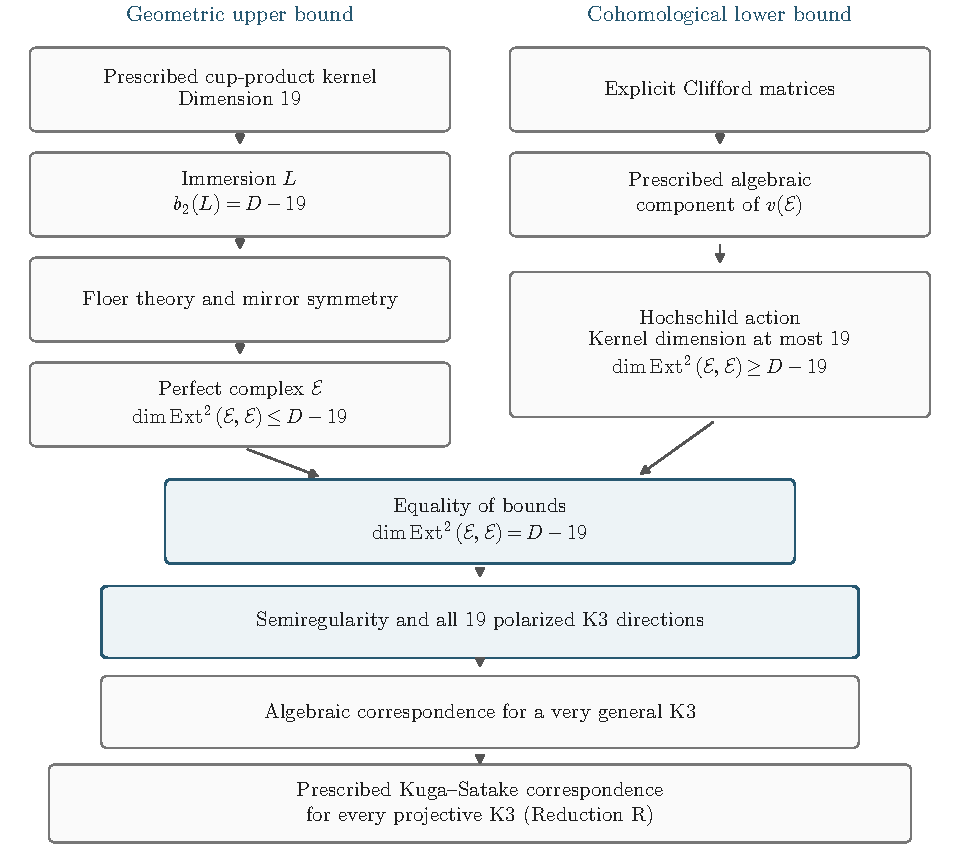
\includegraphics[width=.9\textwidth]{figures/proof-architecture.pdf}
 \caption{The two bounds that produce deformation.  The topological
 construction bounds the second extension group from above; the
 prescribed Mukai component bounds the kernel of the Hochschild
 action from above.  Together they force equality and
 semiregularity.  Here $D=D_{\mathrm{tot}}$.}
 \label{fig:proof-architecture}
\end{figure}

\subsection{Technical contributions and organization}

The construction of algebraic classes through immersed Floer
objects is related to the method in~\cite{W}.  The additional
requirement here is deformation across the full polarized K3
period space.  Prescribing the second Betti number of the
immersion and matching it with the Hochschild calculation
provides that deformation mechanism.

Two analytic details are developed separately because they are
needed to apply the fixed mirror-symmetry theorems to the
constructed immersion.  The first is homological detection of
the immersed obstruction using an interior-marked disk identity.
Finite constructions use both energy and arity bounds; a
coarsened residue of an ultrapower turns successively accurate
solutions into an uncurved object while retaining the trace
pairings needed for representability.  The second is a
comparison between the clean immersed category and the ordinary
categories in the mirror-symmetry theorems.  We verify the
parameterized disk constructions and recover full categories
from ordered Hamiltonian copies.  These statements concern
finite clean collections and may be useful independently of the
K3 application.

Section~\ref{sec:mirror} fixes the mirror varieties, the algebraic
and symplectic cohomology dictionaries, and the generating labels.
Section~\ref{sec:clifford} constructs the matrices and the
cohomology class $\alpha$.  Section~\ref{sec:topology} realizes
its prescribed kernel geometrically.
Sections~\ref{sec:floer} and~\ref{sec:comparison} supply the
Floer construction and category comparisons just described.
Section~\ref{sec:perfect} constructs $\mathcal E$ and computes
the required part of its Mukai vector.
Section~\ref{sec:deformation} proves semiregularity, carries out
the deformation and spreading argument, and establishes
Theorem~\ref{thm:main}.

All cohomology is rational unless another field is indicated.
Floer categories are integrally graded, spin, and use background
class zero.  Their perfect hulls include direct summands.  We
quote the foundational virtual-chain and homological
mirror-symmetry theorems with their needed hypotheses at the
points of application, and prove the extensions specific to the
present construction there.


\section{The starting mirrors and their numerical classes}\label{sec:mirror}

The symplectic construction will take place on a product of a quartic surface
and a torus.  We first identify a finite collection of embedded product
Lagrangians whose category is the category of perfect complexes on a projective
variety.  We establish the ordinary mirror categories and their
numerical classes.  The resulting assertion for clean product labels
uses the comparison and K\"unneth propositions proved in
Section~\ref{sec:comparison}.  This is the only use of homological mirror symmetry.  The numerical
identifications in this section will later determine part of the Chern character
of a complex from intersection numbers.

Let $P$ be a smooth quartic in $\mathbb P^3$, equipped with the restricted
Fubini--Study form normalized to have integral cohomology class $a$.  Write
\begin{equation}\label{eq:quartic-normalization}
 a^2=q\,\pt_P,\qquad q=4.
\end{equation}
Let $g=512$ and let
\[
 Y=(\R/\Z)^g_x\times(\R/\Z)^g_y,\qquad
 \omega_Y=\sum_{i=1}^g X_iY_i,
 \qquad X_i=dx_i,\quad Y_i=dy_i.
\]
Products of differential forms denote exterior products.  Thus
$M=P\times Y$ has complex dimension $n=g+2=514$ and integral symplectic
class $a+\sum_iX_iY_i$.
Choose a nonzero holomorphic two-form on the initial complex quartic
and the flat holomorphic volume form on the torus.  Their product
trivializes the complex determinant of $TM$.  Transport this
trivialization to other compatible almost complex structures through
the contractible space of compatible structures.  Its homotopy
class is the volume grading used on $M$ and on all its branes.

All Floer categories in this section use the Novikov field $\Lambda$ with
complex coefficients and real exponents, supported on sets locally finite to
the left.  The area coefficient $T^\lambda$ has degree zero.  The branes are
integrally graded and spin, with zero background class.  We use the finite
models and coefficient extensions described in Sections~\ref{sec:floer}
and~\ref{sec:comparison}.  An algebraically closed extension of $\Lambda$ of
cardinality at most continuum is abstractly isomorphic to $\C$; the precise
field argument is recorded in Remark~\ref{rem:complex-coefficients}.  N\'eron--Severi groups
and the numerical lattices below do not change under algebraically closed
extensions of characteristic zero.  Consequently we may make these choices
before making a final identification of the coefficient field with $\C$.
To interpret the Betti and Hodge notation in this section, choose a
temporary abstract identification of its current algebraically closed
coefficient field with $\C$ and transport the varieties to that field.
This identification need not fix the original coefficient copy of
$\C$.  The K3 numerical space is intrinsically
$\Q\oplus\NS(S)_\Q\oplus\Q$, with its unit and point summands;
the torus classes used below are rational combinations of divisor
classes specified by integral matrices.  These are the data retained
under subsequent coefficient extensions.  The Hodge assertions used
here hold for every such temporary realization, because the elliptic
curve remains non-CM.

\subsection{The quartic factor}

We use Seidel's undeformed quartic theorem
\cite[Theorem~1.3]{HMS:SeidelQuartic}.  Its coefficient field is the algebraic
closure of a Laurent-series field, and its mirror is the minimal resolution
of the quotient of the Dwork quartic by the diagonal group of order $16$.
Write $u$ for Seidel's series variable.  His prequantum normalization
in Section~11a uses $\mathcal O(4)$, so his symplectic form is four
times the hyperplane-normalized form used here.  Accordingly we extend
his symplectic coefficients by $f(u)=T^{1/4}$: a disk of area $A$
in our normalization has his area $4A$, and $u^{4A}$ becomes $T^A$.
His theorem also twists the mirror scalar action by an invertible
formal reparametrization $\psi$.  We absorb that twist in the mirror
base map; with his convention that a scalar $\lambda$ acts as
$\psi(\lambda)$, the untwisted mirror base map is $f\circ\psi^{-1}$.
The theorem is obtained by identifying
the endomorphism $A_\infty$ algebras on a collection of $64$ Lagrangian spheres;
these spheres split-generate.  We therefore use its enhanced conclusion,
\begin{equation}\label{eq:quartic-hms}
 \operatorname{Perf}\langle\text{the chosen spheres in }P\rangle
 \simeq\Perf(S),
\end{equation}
where $S$ is the mirror K3 surface over the enlarged coefficient field.
Here and below $\operatorname{Perf}$ of an $A_\infty$ category means its ordinary
split-closed pretriangulated hull.

After this rescaling, the symplectic deformation identification between
smooth quartics permits the use of our specified $P$.  We enlarge the finite sphere collection to include
vanishing spheres spanning $a^\perp\subset H^2(P,\Q)$.  Indeed, the vanishing
cohomology of a Lefschetz pencil of quartics in $\mathbb P^3$ is the orthogonal
complement of the hyperplane class.  Its vanishing cycles are Lagrangian
spheres for the restricted K\"ahler form and admit gradings.  They are objects
of Seidel's category: the flat prequantum multisection required there exists
on every sphere.  His theorem identifies the full category, so adding these
objects preserves~\eqref{eq:quartic-hms}.  Scalar extension preserves this
enhanced equivalence and its split-generation assertion, as is seen by
extending a finite perfect resolution of the diagonal.

The mirror family is non-isotrivial, and its geometric generic member has
Picard number at most $19$.  One may use the lattice-polarized mirror-quartic
description for this assertion \cite{HMS:Dolgachev}.  Alternatively, the Dwork
period varies: at the Fermat member its infinitesimal variation is represented
by the product of the four coordinates, which is nonzero in the Jacobian
ring.  The diagonal group is symplectic, and its quotient and crepant resolution
carry the same varying period line.  These correspondences exist in families
after restricting the parameter base.  A non-isotrivial one-parameter K3
family cannot have geometric generic Picard number $20$: a generic divisor
class spreads after a finite base change, whereas the complex K3 surfaces of
Picard number $20$ have only countably many period points.  Seidel's
nonconstant formal parameter, including its invertible change of coordinate,
selects this geometric generic fiber.

Put
\[
 \Lambda_S^{\mathrm{alg}}=H^0(S,\Q)\oplus\NS(S)_\Q\oplus H^4(S,\Q),
 \qquad
 m((r,x,s),(r',x',s'))=xx'-rs'-sr'.
\]
The Euler characteristic of Floer cohomology of two graded Lagrangian
surfaces is minus their oriented intersection number.  The Euler
characteristic on $S$ is minus the Mukai pairing.  Consequently the assignments
of our sphere classes to the Mukai vectors of their mirrors induce a rational
isometry
\begin{equation}\label{eq:mirror-lattice}
 (a^\perp,\cup)\ \xrightarrow{\ \sim\ }\
 (\Lambda_S^{\mathrm{alg}},m).
\end{equation}
For completeness, choose $21$ sphere classes forming a basis of $a^\perp$.
Their intersection matrix is nonsingular, so the matrix of their mirror
Mukai pairings has rank $21$.  Thus $\dim\Lambda_S^{\mathrm{alg}}\ge21$.
The preceding Picard bound gives the reverse inequality.  The resulting
isometry also takes every additional sphere class to its mirror Mukai
vector: pair its difference with the chosen basis and use nondegeneracy.
In particular $\rho(S)=19$.

We specify the Euler sign used here.  In complex dimension $2l$, the sign of
a transverse intersection generator of degree $j$ satisfies
\begin{equation}\label{eq:euler-intersection-sign}
 (-1)^j=(-1)^l\,\operatorname{sign}_{\mathrm{or}}(x).
\end{equation}
This follows by rotating the graded tangent planes to coordinate planes;
each of the $2l$ rotation directions contributes its Maslov crossing sign,
and comparison with the oriented direct-sum convention gives $(-1)^l$.
We always transport orientations with these grading conventions.

\subsection{An ample class in every rational squareclass}

Fix a positive integer $d$ and put $r=2d$.  The rational K3 lattice and Witt cancellation in
\eqref{eq:mirror-lattice} give
\[
 a^\perp\simeq U^2\oplus E_8(-1)^2\oplus\langle-4\rangle,
 \qquad
 \NS(S)_\Q\simeq U\oplus E_8(-1)^2\oplus\langle-4\rangle.
\]
Here $U$ is the hyperbolic plane; it is also the rational Mukai lattice of
$H^0\oplus H^4$.  The quadric $x^2=r$ in $\NS(S)_\R$ has a rational point,
because the rational form contains $U$.  Projection from a rational point
parametrizes a Zariski-open subset of this quadric rationally.  It follows,
using rational points close to the parameters of any real smooth point,
that rational points are dense on each relevant real sheet.  The ample cone
is open and meets the positive sheet.  We can therefore choose
\[
 h\in\NS(S)_\Q\quad\text{ample},\qquad h^2=r.
\]
Clearing denominators and taking the primitive generator of the ray gives
an integral primitive ample class.  Its degree has squareclass $r$; the
normalization $h^2=r$ will be retained in the calculations.

Decompose the Mukai space orthogonally as
\begin{equation}\label{eq:delta-negative}
 \Lambda_S^{\mathrm{alg}}=\Delta\mathbin{\perp}\mathcal N,
 \qquad
 \Delta=H^0(S,\Q)\oplus\Q h\oplus H^4(S,\Q),\qquad
 \mathcal N=h^\perp\cap\NS(S)_\Q.
\end{equation}
Choose any rational basis $d_1,d_2,d_3$ of $\Delta$.  There is a basis
$n_1,\ldots,n_{18}$ of $\mathcal N$ satisfying
\begin{equation}\label{eq:negative-basis}
 m(n_i,n_j)=-\delta_{ij}\lambda_i,
 \qquad (\lambda_1,\ldots,\lambda_{18})=(1,\ldots,1,r).
\end{equation}
To verify this, Witt's theorem moves $h$ into $U$, where its orthogonal
line has squareclass $-r$.  Each rational $E_8$ form is the standard sum of
eight squares: use its usual full-rank lattice in $\Q^8$ with Euclidean
form.  The remaining line $\langle-4\rangle$ is rationally
$\langle-1\rangle$.  This gives seventeen negative unit squares and one
negative square of size $r$.  Through~\eqref{eq:mirror-lattice}, the same
symbols $d_l,n_i$ will denote degree-two classes on $P$.

\subsection{The torus factor and graph objects}

The mirror of $Y$ is
\[
 B=E^g,
\]
where $E$ is the Tate elliptic curve with parameter $T$, the area-one
Novikov parameter.  After any final identification of the coefficient field
with $\C$, $E$ is non-CM.  Indeed its $j$-series is transcendental over the
original complex coefficient field, hence also over $\Q$; field
identification preserves the latter property, whereas a CM $j$-invariant
is algebraic.  Thus the Hodge group of $B$ is the diagonal $SL_2$ acting
on the $g$ copies of $H^1(E)$.

Choose forms $z\in H^{1,0}(E)$ and $w\in H^{0,1}(E)$ once on $E$,
normalized so that $zw$ is its principal polarization class, and
let $z_i,w_i$ be their pullbacks from the $i$th factor of $B$.
Thus the normalization is coherent across all factors.  Define
\begin{equation}\label{eq:matrix-divisors}
 B(A)=z^tAw,\qquad \theta=B(I).
\end{equation}
If $A$ is symmetric integral, $B(A)$ is the divisor class described by
$A$ under the principal polarization of $E^g$.  The rational Hodge algebra
of $B$ is generated by these classes.  Indeed the invariants of the
standard $SL_2$ tensor representation are generated by the alternating
pairings of two factors.  Passing from tensor powers to exterior powers
shows that all invariants in $H^*(B)$ are generated by the corresponding
degree-two classes; on $E^g$ these are exactly the symmetric matrix
divisors.  In particular the classes $e^{B(A)}$, as $A$ ranges over
symmetric integral matrices, span the entire rational Hodge-class space.
This last assertion follows as well by polarizing the finite exponential
polynomial: its coefficients are all products of divisor classes.

For a symmetric integral matrix $A$, let $D_A\subset Y$ be the graph
$y=Ax$ modulo $\Z^g$, with trivial local system and spin structure induced
by the base framing.  Small exact periodic perturbations replace it by
$y=Ax+\nabla f(x)$.  These remain Hamiltonian isotopic graphs.  The inclusion
of any such section induces an injection on fundamental groups, so
$\pi_2(Y,D_A)=0$.  The sections and the torus fibers are therefore
tautologically unobstructed.  The base has $\pi_2=0$, and its framing and
the zero section trivialize the twists in the family Floer construction.

Abouzaid's finite-list $A_\infty$ functor
\cite[Theorem~2.10 and the chain-level construction]{HMS:AbouzaidFaithful}
is cohomologically faithful on these objects.  His fully faithful theorem
\cite[Theorem~1.1 and Corollary~1.2]{HMS:AbouzaidHMS} also applies.  These are undeformed
theorems for our fixed torus fibration.  Its rigid analytic mirror has the
independent multiplicative periods $T$ in each coordinate, and is the
analytification of $B$.  Projective rigid GAGA identifies the resulting
perfect complexes with algebraic ones.  Opposite boundary-order conventions
are matched by taking the $A_\infty$ opposite and perfect duality.

Each $D_A$ meets each fiber once and transversely.  Its local family Floer
complex is consequently a line in one degree.  Its image is a shifted
line bundle, with numerical Chern class
\begin{equation}\label{eq:graph-mirror-class}
 c_1(\mathcal L_A)=\epsilon B(A),\qquad \epsilon\in\{1,-1\}
\end{equation}
for a single sign determined by conventions.  We give the numerical
calculation, following \cite[Section~9.1]{W}, to fix what information
is being used.  On the real universal
cover of the base, lift the section to $Ax+\nabla f(x)$ and use the paths
from the zero section given by this lift.  On a contractible overlap with
the same lift, the winding number in the continuation coefficient is zero:
after closing with these paths it is the boundary winding of a disk over
the contractible base cover.  The scalar continuation factors can be
trivialized there.  Under the deck translation $b\in\Z^g$, the change of
lift gives the monomial multiplier $Z^{-\epsilon Ab}$.  The standard theta
line has precisely this character.  One can check all symmetric matrices
by tensoring pullbacks for rank-one symmetric matrices, which span the
integral symmetric matrices.  Equal monomial characters differ by a
scalar character, hence by an element of $\operatorname{Pic}^0(B)$.
This proves~\eqref{eq:graph-mirror-class}; no identification of that
$\operatorname{Pic}^0$ element is needed.

The shifts can be chosen common to our list.  Continue the graph gradings
from the flat volume grading through the Lagrangian graph planes
$\operatorname{graph}(tA)$ in the fixed tangent space.  These planes
remain transverse to the vertical plane, so their intersection
index is constant.  This is a path of tangent planes; it does not
assert an isotopy between closed graph tori of different integral
slopes.  Exact perturbations have tangent planes in the same
contractible space of symmetric graphs.  There is also a check using morphisms.  Choose all
successive slope differences positive definite and include three ordered
scalar slopes.  Opposite Floer and sheaf degree concentrations would
require the same nonzero shift difference between each pair of three
objects, which is impossible.  With matching concentration, all shift
differences are zero.  Remove the common shift.

On such a list faithfulness already proves fullness without using the
stronger theorem.  Between different slopes all Floer intersections lie
in one degree and their number is $|\det(A'-A)|$.  Riemann--Roch and
ample or anti-ample cohomology vanishing give the identical Ext dimensions
for the mirror lines, independently of their $\operatorname{Pic}^0$
twists.  Self Floer and self Ext have the cohomology ranks of a
$g$-torus.  Hence the faithful maps are isomorphisms on all graded Homs.

We require a finite list for two reasons: its images must recover
$\Perf(B)$, and its numerical classes must give enough Euler-pairing
tests to recover a Hodge-class component.  The next lemma arranges
both properties on the same list.

\begin{lemma}\label{lem:graph-generators}
There is a finite set of symmetric integral slopes, with all successive
differences positive definite, whose graph images split-generate
$\Perf(B)$ and whose classes $e^{B(A)}$ span the rational Hodge classes
of $B$.
\end{lemma}
\begin{proof}
For generation, take a vector bundle $G$ which is a split-generator of
$\Perf(B)$ \cite[Section~3.5]{History:ToenVaquie}, and cover it by sums of sufficiently negative powers of
the principal polarization, tensored with arbitrary elements of
$\operatorname{Pic}^0(B)$.  Serre generation holds uniformly in these
twists: apply relative Serre vanishing and generation to the Poincar\'e
bundle over the proper parameter space $\operatorname{Pic}^0(B)$.
Here is the uniform construction, with all twists left arbitrary.
Put $\mathcal P=\operatorname{Pic}^0(B)$, choose the normalized
Poincar\'e line bundle, and put $K_0=G$.  Suppose that $K_j$ has
been constructed as a vector bundle on $B\times\mathcal P^j$.
Pull it back to $B\times\mathcal P^{j+1}$, and denote the new
Poincar\'e line by $P_{\mathrm{new}}$.  If $H$ represents the
principal polarization and $p$ is projection to
$\mathcal P^{j+1}$, relative Serre vanishing and generation
permit a sufficiently large $m_j$ such that
\[
 F_j=p_*(K_j\otimes H^{m_j}\otimes P_{\mathrm{new}}^{-1})
\]
is locally free, commutes with base change, and has surjective
evaluation.  Tensoring that evaluation gives a surjection
\[
 V_j=p^*F_j\otimes H^{-m_j}\otimes P_{\mathrm{new}}
 \longrightarrow K_j.
\]
Its kernel $K_{j+1}$ is a vector bundle.  This construction is
uniform over the proper parameter space $\mathcal P^{j+1}$,
and $m_j$ may be increased arbitrarily.  After $g+1$ steps,
every tuple of twists gives the required sequence of
surjections; the fiber of $V_j$ is a sum of the prescribed
line $H^{-m_j}\otimes P_j$.  Thus all powers have been chosen
before the unknown graph-image twists are specified.

The resulting exact sequence has the form
\[
 0\longrightarrow K\longrightarrow V_g\longrightarrow\cdots
 \longrightarrow V_0\longrightarrow G\longrightarrow0,
\]
where each $V_j$ is a sum of one of the chosen lines.  Its class in
$\Ext^{g+1}(G,K)$ vanishes because $G$ is locally free and $\dim B=g$.
The corresponding truncated complex of the $V_j$ therefore has $G$
as a direct summand.  These lines split-generate.  Positive powers work
by duality.  This accommodates either sign in
\eqref{eq:graph-mirror-class} and allows the scalar slopes to be as
far apart as desired.

For spanning, the exponential polynomial and divisor generation above
show that all integral symmetric slopes span the Hodge-class space.
The integral points in any translate of the positive-definite cone
are Zariski dense in the vector space of symmetric matrices.  For
example, dilates of a small rational box inside that cone provide
arbitrarily large Cartesian grids, which cannot lie in the zero set
of a fixed nonzero polynomial.  Inductively choose the next slope
outside the annihilating polynomial conditions for the span already
obtained and with positive-definite difference from every preceding
slope.  Finitely many choices suffice.  Append them to the scalar
slopes used for generation.
\end{proof}

\subsection{The cohomology dictionary and rational areas}

For computations on the symplectic torus, regard $z_i,w_i$ as formal
exterior generators and define the rational vector-space isomorphism
\begin{equation}\label{eq:complement-transform}
 F(\gamma)=
 \gamma\bigl(\iota_{\partial/\partial Y_i},X_i\wedge\bigr)
 (Y_1\cdots Y_g).
\end{equation}
Here a monomial is evaluated in its displayed exterior order.
Multiplication by $Y_i$ after applying $F$ corresponds to
$\partial_{z_i}$ before applying $F$, and multiplication by $X_i$
corresponds to left multiplication by $w_i$.  Direct expansion gives
\begin{equation}\label{eq:graph-class}
 F(e^{B(A)})=\prod_{i=1}^g\left(Y_i-\sum_jA_{ij}X_j\right).
\end{equation}
This is the Poincar\'e dual of $D_A$, up to one orientation convention
independent of $A$.  In particular graph intersections and Euler
pairings of the mirror lines are both the determinant pairing in
the slope matrices, with the common sign already specified.

The numerical dictionary is now fixed.  Before collecting the mirror
input, we arrange the discrete polygon-area groups used by the finite
category comparisons in Section~\ref{sec:comparison}.

\begin{lemma}\label{lem:rational-label-areas}
The finite sphere and graph collections above can be put in transverse
position, without triple intersections, so that polygon areas on
each finite collection lie in a fixed discrete rational subgroup of
$\R$.  Their product collection is clean and has the same property.
The construction can be made successively for countably many
Hamiltonian copies, with a denominator depending on the finite
subcollection.
\end{lemma}
\begin{proof}
Use integral prequantum bundles.  A sphere has trivial flat holonomy.
On an undisplaced integral symmetric graph, the quadratic primitive
on the real cover gives rational holonomy (the offsets are
half-integral).  Thus a finite prequantum power has a parallel section
on each label.  Hamiltonian perturbation preserves this property.
First arrange transverse position and no triples.  At each of the
finitely many intersection points, compare the values of the chosen
parallel sections.  Small exact graph perturbations in Weinstein
neighborhoods of the labels make all these
phase differences rational: take functions constant near each
intersection preimage, with separately prescribed constants and
disjoint supports there.  Their differentials vanish near the
intersections, so the intersection positions are unchanged, while
the continued prequantum sections change phase by the corresponding
endpoint primitive differences.  There are no triples, hence the
phase conditions at distinct pair intersections are independent.
Choose rational target phases sufficiently close to the original
ones to keep all transversality conditions.  For torus labels these
are exact periodic perturbations.

After passing to a common power, all phase ratios are roots of unity.
Parallel transport around a polygon boundary therefore gives its
symplectic area in $D^{-1}\Z$ for a fixed $D>0$.  This argument allows
switches between labels at corners.  The tensor product prequantum
sections give the assertion for product labels: their intersections
are products of clean components, and the phase ratios are constant
roots of unity on each component.  At each new layer of Hamiltonian
copies only finitely many old intersections impose conditions;
performing the construction successively proves the last assertion.
\end{proof}

\begin{proposition}[Starting mirror category]\label{prop:mirror-input}
For every integer $d>0$ there exist finite collections of graded spin
spheres in $P$ and graded spin graph tori in $Y$, an algebraically closed
extension $k\supset\Lambda$ of cardinality at most continuum, a projective
K3 surface $S/k$ of Picard number $19$, and $B=E^g/k$ as above, with
the following properties.
\begin{enumerate}[label=\textup{(\roman*)}]
\item The product labels, with their induced zero-curvature bounding
cochains, form a full subcategory of the clean Fukaya category of
$P\times Y$.  Its ordinary perfect hull is equivalent to
$\Perf(S\times B)$, with all Homs and products respected.
\item The sphere classes and mirror Mukai vectors give
\eqref{eq:mirror-lattice}.  The ample rational class $h$, decomposition
\eqref{eq:delta-negative}, and bases satisfying
\eqref{eq:negative-basis} can be chosen with $h^2=2d$.
\item The graph images are line bundles with numerical classes
$e^{\epsilon B(A)}$, for one common $\epsilon=\pm1$.  They
split-generate $\Perf(B)$, and these classes span all rational
Hodge classes of $B$.  Their symplectic classes are given by
\eqref{eq:graph-class}.
\item Each individual product label has self Floer cohomology with
the full graded ranks of its ordinary cohomology.  The labels obey
the rational-area convention of Lemma~\ref{lem:rational-label-areas}.
\end{enumerate}
\end{proposition}
\begin{proof}
The undeformed sphere and graph calculations above first give the
ordinary categories on each factor.  Proposition~\ref{prop:category-comparison}
identifies these with their finite clean models, preserving the labeled
objects, after a coefficient extension as stated.  Apply
Proposition~\ref{prop:ordinary-kunneth} to the two clean collections.
The exterior products of the two sets of mirror generators
split-generate $\Perf(S\times B)$; this follows, for example, by
taking exterior products of perfect diagonal resolutions.  The full
Hom comparison in that proposition proves~\textup{(i)}.  Parts
\textup{(ii)} and~\textup{(iii)} were proved above.  For~\textup{(iv)},
choose a common compatible almost complex structure on $P$ having
neither spheres nor individual-label disks, as in
\cite[Lemma~8.4]{HMS:SeidelQuartic}.  On $Y$ the relative homotopy argument excludes disks
for every compatible structure.  Each factor label has zero
bounding cochain and self Floer ranks equal to its ordinary
cohomology ranks.  K\"unneth gives the product ranks.  Finally apply
Lemma~\ref{lem:rational-label-areas}.  All coefficient extensions can
be included in one algebraically closed field of cardinality at
most continuum.
\end{proof}


\section{A middle-dimensional class with a prescribed cup-product kernel}
\label{sec:clifford}

We construct a rational class on $M=P\times Y$ whose annihilator in
$H^2(M,\Q)$ has dimension $19$ and contains the symplectic class.
The construction also makes cup product injective on the tensor product
of this annihilator with $H^1(M,\Q)$.  These two properties will control
the second cohomology of the manifold constructed in
Section~\ref{sec:topology}.

We retain the cohomology dictionary of Section~\ref{sec:mirror}.
Thus $g=512$, $n=g+2$, $q=4$, and $a\in H^2(P,\Q)$ satisfies
$a^2=q\pt_P$.  Fix a positive integer $d$ and put
\[
 r=2d,\qquad c=qr,\qquad
 (\lambda_1,\ldots,\lambda_{18})=(1,\ldots,1,r).
\]
Under the isometry \eqref{eq:mirror-lattice}, regard the basis
$d_1,d_2,d_3$ of $\Delta$ and the basis $n_1,\ldots,n_{18}$ of
$\mathcal N$ as classes in $a^\perp\subset H^2(P,\Q)$.
In particular,
\begin{equation}\label{eq:clifford-P-pairings}
 a d_l=a n_i=d_l n_i=0,\qquad
 n_i n_j=-\delta_{ij}\lambda_i\pt_P.
\end{equation}
The products $d_l d_k$ are given by the nondegenerate restriction of
the cup-product form to $\Delta$; their individual values will not be
needed.  All cohomology classes in this section have rational
coefficients unless a field extension is specified.

We will arrange that the annihilator projects isomorphically onto
$\mathcal N\oplus\Q a\subset H^2(P,\Q)$.  Thus its torus component
must be determined uniquely by its nineteen coefficients on $P$.
The following matrices provide the linear relation between these two
components.

\subsection{Rational symmetric Clifford matrices}

The required matrix sizes and square factors matter: the negative
directions $n_i$ have different lengths, and the matrices must compensate
for them.  We use the normed-algebra construction of Clifford matrices
(see, for example, \cite[Sections~2.2--2.3]{Algebra:Baez}), followed by
rational changes of basis.  We give the construction explicitly.

\begin{proposition}\label{prop:clifford-matrices}
There are symmetric matrices $G_1,\ldots,G_{18}\in M_g(\Q)$ such that
\begin{equation}\label{eq:clifford-relations}
 G_i^2=\frac r{\lambda_i}I_g,\qquad
 G_iG_j=-G_jG_i\quad(i\ne j).
\end{equation}
They generate $M_g(\Q)$.  Consequently their common commutant over any
field of characteristic zero is the scalar matrices.  The ordered
product
\begin{equation}\label{eq:K-definition}
 K=\frac{2}{r^8}G_1\cdots G_{18}
\end{equation}
satisfies
\begin{equation}\label{eq:K-identities}
 K^t=-K,\qquad K^2=-cI_g,\qquad KG_i=-G_iK.
\end{equation}
\end{proposition}

\begin{proof}
First construct eight symmetric anticommuting involutions on $\Q^{16}$.
Let $\mathbb H_{\Q}$ be the quaternion algebra with basis $1,i,j,k$,
relations $i^2=j^2=k^2=ijk=-1$, and norm
$|a|^2=a\bar a$.  On
$\mathbb O_{\Q}=\mathbb H_{\Q}\oplus\mathbb H_{\Q}$ use the product
\[
 (a,b)(u,v)=(au-\bar v b,\;va+b\bar u)
\]
and the norm $|(a,b)|^2=|a|^2+|b|^2$.
This norm is multiplicative.  Indeed, on expanding the two squared
norms, their mixed terms are
$-2\operatorname{Re}(au\bar b v)$ and
$2\operatorname{Re}(vau\bar b)$, which cancel because the real part of
a product of quaternions is invariant under cyclic permutation.
The remaining four terms give
$(|a|^2+|b|^2)(|u|^2+|v|^2)$.

Use the standard orthonormal rational basis $e_1,\ldots,e_8$ of
$\mathbb O_{\Q}$, and let $L_x$ be the $8\times8$ matrix of left
multiplication by $x$.  Multiplicativity gives
$L_x^tL_x=|x|^2I_8$.  For $x\ne0$ it also gives
$L_xL_x^t=|x|^2I_8$, by invertibility; the latter equality is automatic
at $x=0$.  Polarizing both identities shows that
\[
 L_x^tL_y+L_y^tL_x=2\langle x,y\rangle I_8,
 \qquad
 L_xL_y^t+L_yL_x^t=2\langle x,y\rangle I_8.
\]
It follows that the rational symmetric matrices
\[
 A_j=\begin{pmatrix}0&L_{e_j}^t\\L_{e_j}&0\end{pmatrix}
 \quad(1\le j\le8)
\]
satisfy $A_iA_j+A_jA_i=2\delta_{ij}I_{16}$.
Their product $J_8=A_1\cdots A_8$ is symmetric, has square $I_{16}$,
and anticommutes with every $A_j$: reversing eight factors gives the
sign $(-1)^{28}=1$, and commuting a chosen factor through the other
seven gives the sign $-1$.

On $\Q^{16}\otimes\Q^{16}$ define sixteen matrices
\[
 T_j=A_j\otimes I_{16},\qquad
 T_{8+j}=J_8\otimes A_j\quad(1\le j\le8).
\]
They are symmetric anticommuting involutions.  Their product
$J_{16}=T_1\cdots T_{16}$ is a symmetric involution anticommuting with
each $T_j$, since $(-1)^{120}=1$ and $(-1)^{15}=-1$.

By Lagrange's four-square theorem, choose integers
$b_0,b_1,b_2,b_3$ with $r=b_0^2+b_1^2+b_2^2+b_3^2$.
The matrix of multiplication by the corresponding quaternion is
\[
 Q_r=\begin{pmatrix}
 b_0&-b_1&-b_2&-b_3\\
 b_1&b_0&-b_3&b_2\\
 b_2&b_3&b_0&-b_1\\
 b_3&-b_2&b_1&b_0
 \end{pmatrix},\qquad
 Q_rQ_r^t=Q_r^tQ_r=rI_4.
\]
For $0\le a\le3$ and $1\le i\le4$, replace each block of four
generators by
\[
 U_{4a+i}=\sum_{j=1}^4(Q_r)_{ij}T_{4a+j}.
\]
The orthogonality of the rows of $Q_r$ gives
$U_iU_j+U_jU_i=2r\delta_{ij}I_{256}$.  The $U_i$ remain symmetric,
and each anticommutes with $J_{16}$.

Equip $\Q^{256}\otimes\Q^2$ with the symmetric form of matrix
$H=I_{256}\otimes\operatorname{diag}(1,r)$.  The eighteen matrices
\[
 \widetilde G_i=U_i\otimes I_2\quad(1\le i\le16),\qquad
 \widetilde G_{17}=J_{16}\otimes
     \begin{pmatrix}0&r\\1&0\end{pmatrix},\qquad
 \widetilde G_{18}=J_{16}\otimes
     \begin{pmatrix}1&0\\0&-1\end{pmatrix}
\]
are self-adjoint for $H$.  They anticommute in pairs, the first seventeen
have square $rI_g$, and the last has square $I_g$.
The form $H$ is rationally isometric to $I_g$: reorder its coordinates
as $I_{256}\oplus rI_{256}$ and use $Q_r/r$ on each four-dimensional
block of the second summand.  Indeed
$(Q_r/r)^t(rI_4)(Q_r/r)=I_4$.
Thus there is an explicit rational matrix $V$ with $V^tHV=I_g$.
Set $G_i=V^{-1}\widetilde G_iV$.  Self-adjointness for $H$ now becomes
ordinary symmetry, and \eqref{eq:clifford-relations} follows.

To prove generation without using a classification of Clifford algebras,
write $G_I=G_{i_1}\cdots G_{i_k}$ for
$I=\{i_1<\cdots<i_k\}\subset\{1,\ldots,18\}$, with $G_\varnothing=I_g$.
Every nonempty $G_I$ has trace zero.  If $|I|$ is even, conjugation by
any $G_j$ with $j\in I$ changes its sign.  If $|I|$ is odd, choose
$j\notin I$; such a $j$ exists because $18$ is even, and conjugation
again changes its sign.  Each $G_j$ is invertible, so trace invariance
proves the assertion.  If $I\ne J$, the product $G_IG_J$ is a nonzero
rational multiple of $G_{I\mathbin{\triangle}J}$ and hence has trace
zero.  In contrast, $G_I^2$ is a nonzero rational scalar matrix.
The $2^{18}=g^2$ matrices $G_I$ are therefore linearly independent,
as one sees by multiplying a linear relation by $G_J$ and taking its
trace.  They form a basis of $M_g(\Q)$.  Generation and the commutant
assertion follow, also after extension of scalars.

Finally, reversing the eighteen factors introduces
$(-1)^{153}=-1$, and commuting a generator through the other seventeen
introduces $-1$.  Since
$\prod_i(r/\lambda_i)=r^{17}$, we obtain
\[
 K^t=-K,\qquad
 K^2=\frac4{r^{16}}(-1)^{153}r^{17}I_g=-4rI_g=-cI_g.
\]
This also proves the anticommutation in \eqref{eq:K-identities}.
\end{proof}

\subsection{Separating the exterior-algebra operators}

Recall the formal exterior generators $z_1,\ldots,z_g,w_1,\ldots,w_g$,
the forms $B(A)=z^tAw$ and $\theta=\sum_i z_iw_i$, and the complement
transform $F$ of \eqref{eq:complement-transform}.
For a skew matrix $C$ put
\[
 W(C)=\frac12\sum_{i,j}C_{ij}w_iw_j,\qquad
 Z(C)=\frac12\sum_{i,j}C_{ij}z_iz_j.
\]
Both assignments are injective on skew matrices.  For any matrix $D$
and any skew matrix $R$, define operators on the exterior algebra by
\begin{equation}\label{eq:exterior-operators}
 e_D=\sum_{i,j}D_{ij}w_i\partial_{z_j},\qquad
 A_2(C,R,D)=W(C)\wedge(-)
       +\frac12\sum_{i,j}R_{ij}\partial_{z_i}\partial_{z_j}+e_D.
\end{equation}
Here $\partial_{z_i}$ is the left exterior derivative:
$\partial_{z_i}(uv)=(\partial_{z_i}u)v+(-1)^{\deg u}u\partial_{z_i}v$.
Products of operators act on the rightmost input first.

These are precisely the operators obtained by transporting multiplication
by a degree-two torus class through $F$.  In fact the anticommutation
relations for exterior multiplication and contraction give
\[
 X_iF(\gamma)=F(w_i\gamma),\qquad
 Y_iF(\gamma)=F(\partial_{z_i}\gamma).
\]
For the second identity, commute $Y_i\wedge(-)$ through the substituted
operators in the definition of $F$; its anticommutator with
$\iota_{\partial/\partial Y_j}$ is $\delta_{ij}$, and it kills the
vacuum $Y_1\cdots Y_g$.  Thus multiplication by
\begin{equation}\label{eq:torus-general-degree-two}
 \frac12X^tCX+X^tDY+\frac12Y^tRY
\end{equation}
corresponds to $A_2(C,R,D)$, with the displayed signs.

Choose pairwise disjoint sets $J_1,J_2,J_3$, each consisting of three
distinct positive integers, and put
\begin{equation}\label{eq:beta-definition}
 \beta_l=\sum_{j\in J_l}e^{j\theta}\quad(1\le l\le3).
\end{equation}
The exponential is the finite exterior-algebra sum
$e^{j\theta}=\sum_{k=0}^g j^k\theta^k/k!$.
Three distinct coefficients in each sum will eliminate the three
matrix parameters $C$, $R$, and $D-D^t$.

\begin{lemma}\label{lem:exponential-elimination}
Let $k$ be a field of characteristic zero, let $g\ge10$, and let
$J_1,J_2,J_3\subset k^\times$ be pairwise disjoint sets of three
distinct elements.  Define $\beta_l$ by \eqref{eq:beta-definition} in
$\bigwedge_k\langle z_1,\ldots,z_g,w_1,\ldots,w_g\rangle$.
For skew matrices $C,R$, an arbitrary matrix $D$, scalars $s_l$, and
an arbitrary exterior form $\rho$, the equations
\begin{equation}\label{eq:exponential-elimination-system}
 A_2(C,R,D)\beta_l+s_l\rho=0\qquad(1\le l\le3)
\end{equation}
imply
\[
 C=R=0,\qquad D=D^t,\qquad s_l\rho=0\quad(1\le l\le3).
\]
Moreover, the three $\beta_l$ are linearly independent modulo the
subspace of exterior forms of degrees at most two.
\end{lemma}

\begin{proof}
Write $U=\bigwedge^2\langle w_1,\ldots,w_g\rangle$.
We first show that the nine subspaces $e^{j\theta}U$, for
$j\in J_1\cup J_2\cup J_3$, have direct sum.
The elementary Lefschetz fact needed here is that
\begin{equation}\label{eq:restricted-lefschetz}
 U\longrightarrow\bigwedge^{2k+2}\langle z,w\rangle,\qquad
 u\longmapsto\theta^ku
 \quad\hbox{is injective for }0\le k\le g-2.
\end{equation}
To see this directly, write $u=\sum_{a<b}u_{ab}w_aw_b$.
For each pair $a<b$, choose $k$ indices distinct from $a,b$.
The coefficient in $\theta^ku$ with exactly these $z$-indices and
with these $w$-indices together with $a,b$ is $\pm k!u_{ab}$.
No other coefficient of $u$ contributes.  This proves injectivity.
Now suppose $\sum_j e^{j\theta}u_j=0$ with $u_j\in U$.
Taking total exterior degrees $2,4,\ldots,18$ and applying
\eqref{eq:restricted-lefschetz} gives
\[
 \sum_j j^k u_j=0\qquad(0\le k\le8).
\]
The Vandermonde matrix is invertible because the nine $j$'s are
distinct, so every $u_j$ is zero.

Our sign convention for exterior derivatives gives
\[
 \partial_{z_i}e^{j\theta}=j w_i e^{j\theta},\qquad
 \partial_{z_i}\partial_{z_h}e^{j\theta}
       =j^2w_iw_he^{j\theta}.
\]
The minus sign from differentiating past $w_h$ in the second formula
is canceled by interchanging $w_h$ and $w_i$.
It follows that
\begin{equation}\label{eq:A2-exponential}
 A_2(C,R,D)e^{j\theta}
   =e^{j\theta}W\bigl(C+j(D-D^t)+j^2R\bigr).
\end{equation}
In particular $A_2\beta_l$ lies in
$V_l=\bigoplus_{j\in J_l}e^{j\theta}U$, and the three $V_l$ have
direct sum.  If $\rho=0$, each $A_2\beta_l$ vanishes.
If $\rho\ne0$, at most one of the $s_l$ can be nonzero: two nonzero
ones would place $\rho$ in the intersection of two distinct $V_l$.
Thus in either case at least one $A_2\beta_l$ vanishes.
By the direct sum just proved and \eqref{eq:A2-exponential}, the
matrix polynomial
$C+j(D-D^t)+j^2R$ vanishes at the three elements of that $J_l$.
Each entry has degree at most two, so all three coefficient matrices
are zero.  Equation~\eqref{eq:A2-exponential} then makes every
$A_2\beta_l$ zero, and \eqref{eq:exponential-elimination-system}
gives $s_l\rho=0$.

For the final assertion, suppose $\sum_l a_l\beta_l$ has degree at
most two, and set $b_j=a_l$ for $j\in J_l$.
The components of degrees $2k$, $2\le k\le10$, give
$\sum_j b_jj^k=0$, since $\theta^k\ne0$ for $k\le g$.
This coefficient matrix is a Vandermonde matrix multiplied by the
invertible diagonal matrix with entries $j^2$.
Hence $b_j=0$ for every $j$, and every $a_l$ is zero.
\end{proof}

\subsection{The class and its annihilator}

Fix the matrices of Proposition~\ref{prop:clifford-matrices}.  Set
\begin{equation}\label{eq:auxiliary-exterior-forms}
 \chi=\frac2q W(K),\qquad
 \eta=-\frac1q B(K),\qquad
 \nu=Z(K),
\end{equation}
and define
\begin{equation}\label{eq:alpha}
 \alpha=\sum_{l=1}^3 d_lF(\beta_l)
       +\sum_{i=1}^{18}n_iF(B(G_i))
       +F(\chi)+aF(\eta)+\pt_PF(\nu).
\end{equation}
Products in this formula mean exterior products from the two factors
of $M$.  Although $\beta_l$ has components in several exterior
degrees, $\alpha$ is homogeneous of cohomological degree $n$.
Indeed, a monomial with $p$ $z$-factors and $s$ $w$-factors has image
under $F$ in degree $g-p+s$.  The first two groups in
\eqref{eq:alpha} therefore have torus degree $g$; the last three
have torus degrees $g+2,g,g-2$, respectively.  The accompanying
$P$-degrees are $2,2,0,2,4$, so every term has degree $g+2=n$.
All coefficients are rational.

The terms of \eqref{eq:alpha} serve three purposes in the kernel
calculation.  The $\Delta$-terms, together with $\chi\ne0$, allow
Lemma~\ref{lem:exponential-elimination} to remove the $\Delta$-coordinates,
the $XX$- and $YY$-components, and the skew part of the torus matrix.
The $\mathcal N$-terms then turn the coefficients of the $n_i$ into
commutator equations involving $G_i$.  Finally,
$F(\chi)+aF(\eta)+\pt_PF(\nu)$ couples these equations so that the
surviving torus matrix is uniquely determined by arbitrary coefficients
in $\mathcal N\oplus\Q a$.  The proof below verifies each of these claims.

\begin{proposition}\label{prop:cup-kernel}
Let $\alpha\in H^n(M,\Q)$ be the class \eqref{eq:alpha}, where
$M=P\times Y$, $g=512$, and $n=g+2$.  Put
\[
 D_{\mathrm{tot}}=\dim H^2(M,\Q)=22+\binom{2g}{2}.
\]
The kernel of
$\alpha\cup(-):H^2(M,\Q)\longrightarrow H^{n+2}(M,\Q)$ is
\begin{equation}\label{eq:omega}
 \Omega=\left\{
   \sum_{i=1}^{18}t_i n_i+ua+X^tDY:
   D=uI_g+K^{-1}\sum_{i=1}^{18}\lambda_i t_iG_i,
   \quad t_i,u\in\Q\right\}.
\end{equation}
Consequently $\dim\Omega=19$, and $\Omega$ contains the symplectic
class $a+\sum_iX_iY_i$.  Furthermore cup product induces an injection
\begin{equation}\label{eq:omega-h1-injective}
 \Omega\otimes H^1(M,\Q)\longrightarrow H^3(M,\Q).
\end{equation}
\end{proposition}

\begin{proof}
Since $H^1(P,\Q)=0$, every degree-two class on $M$ has a unique
expression
\[
 x=\sum_{l=1}^3s_ld_l+\sum_{i=1}^{18}t_in_i+ua
      +\frac12X^tCX+X^tDY+\frac12Y^tRY,
\]
where $C,R$ are skew and $D$ is arbitrary.  Let
$A_2=A_2(C,R,D)$.
Project $x\alpha$ to the $\Delta$-summand of its degree-two
$P$-component, and apply $F^{-1}$ to the torus factor.
The resulting equations are
\[
 s_l\chi+A_2\beta_l=0\qquad(1\le l\le3).
\]
Here $s_l\chi$ comes from multiplying the $P$-component of $x$ by
$F(\chi)$, and the other term comes from the torus component of $x$.
Since $K$ is invertible and skew, $W(K)\ne0$.
Lemma~\ref{lem:exponential-elimination} therefore gives
\begin{equation}\label{eq:kernel-first-reduction}
 s_1=s_2=s_3=0,\qquad C=R=0,\qquad D=D^t.
\end{equation}

We now compute the remaining components, keeping the exterior signs
explicit.  For symmetric $D$ and $G$, differentiation and reordering
give
\[
 \begin{aligned}
 e_DB(G)&=\sum_{i,j,b}D_{ij}G_{jb}w_iw_b
                 =W(DG-GD),\\
 e_DB(K)&=\sum_{i,j,b}D_{ij}K_{jb}w_iw_b
                 =W(DK+KD),\\
 e_DZ(K)&=\sum_{i,j,b}D_{ij}K_{jb}w_iz_b
                 =B(KD),\\
 e_DW(K)&=0.
 \end{aligned}
\]
For the third equality, $\partial_{z_j}Z(K)=\sum_bK_{jb}z_b$;
moving $w_i$ past $z_b$ gives the coefficient matrix
$-(DK)^t=KD$.  In the first two equalities we used
$\sum_{i,b}A_{ib}w_iw_b=W(A-A^t)$.

Using \eqref{eq:clifford-P-pairings}, the degree-zero, degree-two, and
degree-four $P$-components of $x\alpha=0$, after
\eqref{eq:kernel-first-reduction}, are exactly
\[
 \begin{array}{c|l}
 \text{$P$-component}&\text{equation before applying $F$}\\ \hline
 1&e_D\chi=0,\\
 n_i&t_i\chi+e_DB(G_i)=0,\\
 a&u\chi+e_D\eta=0,\\
 \pt_P&-\displaystyle\sum_i\lambda_it_iB(G_i)+qu\eta+e_D\nu=0.
 \end{array}
\]
The first equation is automatic.  The remaining equations are
equivalent, by injectivity of $W$ on skew matrices and of $B$ on all
matrices, to
\begin{equation}\label{eq:kernel-matrix-equations}
 \begin{aligned}
 [D,G_i]&=-\frac2q t_iK\quad(1\le i\le18),\\
 DK+KD&=2uK,\\
 KD&=uK+\sum_i\lambda_it_iG_i.
 \end{aligned}
\end{equation}
The last equation determines $D$ uniquely as in \eqref{eq:omega}.
It remains to check that it imposes no further conditions on $u,t_i$.

Write $A=\sum_i\lambda_it_iG_i$ and $D=uI_g+K^{-1}A$.
Both $A$ and the $G_i$ are symmetric, and $AK=-KA$.
Since $(K^{-1})^t=-K^{-1}$, we have
\[
 (K^{-1}A)^t=-AK^{-1}=K^{-1}A,
\]
so $D$ is symmetric.  Anticommutation also gives
$K^{-1}AK=-A$, whence $DK+KD=2uK$.
For the first equation of \eqref{eq:kernel-matrix-equations}, use
$G_iK^{-1}=-K^{-1}G_i$ and \eqref{eq:clifford-relations} to obtain
\[
 \begin{aligned}
 [K^{-1}A,G_i]
   &=K^{-1}(AG_i+G_iA)
     =2\lambda_it_i\frac r{\lambda_i}K^{-1}\\
   &=2rt_iK^{-1}
     =-\frac2q t_iK,
 \end{aligned}
\]
where $K^{-1}=-K/c$ and $c=qr$.
Finally $KD=uK+A$ by definition.  Thus every choice of $u,t_i$
satisfies all the equations, proving \eqref{eq:omega}.

Projection of $\Omega$ to $H^2(P,\Q)$ identifies it with
$\mathcal N\oplus\Q a$, so its dimension is $19$.
Taking $t_i=0$ and $u=1$ yields the symplectic class.
For the last assertion, use $H^1(M,\Q)=H^1(Y,\Q)$ and project
the proposed cup product to
$H^2(P,\Q)\otimes H^1(Y,\Q)\subset H^3(M,\Q)$.
On $\Omega\otimes H^1(Y,\Q)$ this projection is the tensor product
of the injective projection $\Omega\to H^2(P,\Q)$ with the identity.
It is injective, proving \eqref{eq:omega-h1-injective}.
\end{proof}

The construction supplies a rational $19$-dimensional subspace
$\Omega$ with $\Omega\alpha=0$ and no relations after multiplying
by $H^1(M,\Q)$.  These are the precise cohomological properties used
to realize a multiple of $\alpha$ by an immersed Lagrangian in the
next section.  The matrices and Lemma~\ref{lem:exponential-elimination}
will also be used in the deformation calculation.


\section{A graded immersed representative with controlled second cohomology}
\label{sec:topology}

We now realize the middle-dimensional class constructed in
Section~\ref{sec:clifford} by a Lagrangian immersion.  Two features of the
representative will be used in the Floer argument: its second Betti number
is prescribed, and its double points contribute no even-degree generators.
The latter condition will be obtained without performing surgery on the
Lagrangian double points, so that the former condition is retained.

Throughout this section homology and cohomology have rational coefficients
unless indicated otherwise.  Put
\[
 M=P\times Y,\qquad g=512,\qquad n=g+2=514,
 \qquad \omega=\omega_P+\omega_Y.
\]
The form is normalized so that $[\omega]$ is integral.  We use the
determinant trivialization and grading convention fixed in
Section~\ref{sec:mirror}.  Let $\alpha\in H^n(M;\Q)$ and
$\Omega\subset H^2(M;\Q)$ be the class and subspace in
\eqref{eq:alpha} and \eqref{eq:omega}.  The properties from
Proposition~\ref{prop:cup-kernel} needed here are
\begin{equation}\label{top:eq:inputs}
 \begin{gathered}
 \ker\bigl(\alpha\cup-:H^2(M)\longrightarrow H^{n+2}(M)\bigr)=\Omega,
 \qquad \dim\Omega=19,\qquad [\omega]\in\Omega,\\
 \Omega\otimes H^1(M)\longrightarrow H^3(M),
 \qquad \zeta\otimes v\longmapsto\zeta\cup v,
 \quad\text{is injective}.
 \end{gathered}
\end{equation}
Write $D_{\mathrm{tot}}=22+\binom{2g}{2}=b_2(M)$.  Fix the finite
list $\mathcal D$ of embedded product labels from
Section~\ref{sec:mirror}, with the rational prequantization data of
Lemma~\ref{lem:rational-label-areas}.

\begin{proposition}\label{prop:immersion}
There are a closed connected oriented spin $n$-manifold $L$, a positive
integer $\mu$, and an integrally graded Lagrangian immersion $i:L\to M$
with the following properties.
\begin{enumerate}[label=\textup{(\roman*)}]
 \item The immersion is self-transverse, has only double points, and
 \[
       \PD(i_*[L])=\mu\alpha.
 \]
 \item Pullback induces an isomorphism
 \[
       H^2(M)/\Omega\xrightarrow{\ \sim\ }H^2(L).
 \]
 In particular, $b_2(L)=D_{\mathrm{tot}}-19$.  Pushforward
 $i_*:H_{n-2}(L)\to H_{n-2}(M)$ is injective.
 \item The two ordered intersection degrees at every double point are
 odd.
 \item The immersion is transverse to each member of $\mathcal D$.
 Its double values avoid those labels, and its intersections with them
 avoid intersections between distinct labels.  There is an integer
 $N_0>0$ such that the symplectic area of every piecewise smooth disk
 whose boundary lifts, between successive corners, to members of
 $\mathcal D\cup\{i\}$ belongs to $N_0^{-1}\Z$.
\end{enumerate}
Here an immersion boundary segment is specified by a lift to its source;
corners may switch between the two preimages of a double point.
\end{proposition}

The topology and local handle construction adapt
\cite[Lemmas~3.3--3.6]{W}.  The adaptations requiring proof are that $M$
has nontrivial tangent bundle and nonzero second homotopy group.  We first
construct the source with its prescribed stable tangent bundle, then
arrange zero-area filling classes explicitly, and finally carry out the
local replacement inside a contractible domain.

\subsection{The torus bundle and a tangentially prescribed representative}

Choose linearly independent integral classes $e_1,\ldots,e_{19}$ spanning
$\Omega$ over $\Q$.  Let
\[
                  \pi:\widehat M\longrightarrow M
\]
be the principal $(S^1)^{19}$-bundle with these Chern classes.  The purpose
of this bundle is to kill exactly the unwanted degree-two classes while
retaining a lift of the required fundamental class.

\begin{lemma}\label{top:lem:bundle}
Pullback identifies $H^2(\widehat M)$ with $H^2(M)/\Omega$.  Moreover,
$\PD(\alpha)\in H_n(M)$ belongs to the image of
$\pi_*:H_n(\widehat M)\to H_n(M)$.
\end{lemma}

\begin{proof}
The manifold $M$ admits a compact K\"ahler structure, independently of
the almost complex structures later used for holomorphic curves.  Its
de Rham algebra is therefore formal
\cite[Section~6, Main Theorem]{Top:DGMS}.  The connection
model for a principal torus bundle, combined with formality, gives the
finite-dimensional real differential graded algebra
\begin{equation}\label{top:eq:hirsch}
 \mathcal A=H^*(M;\R)\otimes\bigwedge(t_1,\ldots,t_{19}),
 \qquad |t_j|=1,\qquad dt_j=e_j,
\end{equation}
as a model for $\widehat M$, compatible with pullback from $M$;
see \cite[Hirsch Lemma~(3.1) and the principal-fibration discussion]{Top:DGMS}.
To specify this compatibility, a connection on the bundle gives the
model $\Omega^*(M)\otimes\bigwedge(t_j)$ with $dt_j$ the curvature
representatives.  Along a formality quasi-isomorphism, replacing a
curvature representative by one differing by $d\beta_j$ is absorbed by
replacing $t_j$ by $t_j+\beta_j$.  Thus the usual Hirsch extension
construction supplies a zigzag respecting the base inclusion.

The degree-two part of \eqref{top:eq:hirsch} is the sum of
$H^2(M)$, $H^1(M)\otimes\Span(t_j)$, and
$\bigwedge^2\Span(t_j)$.  The differential on the second summand is
injective by \eqref{top:eq:inputs}.  Its value lies in $H^3(M)$.
The differential on the third summand lies in
$H^2(M)\otimes\Span(t_j)$ and is injective: the coefficient of each
$t_j$ is a linear combination of the independent $e_i$, and its
vanishing makes all coefficients of the original exterior two-form
zero.  These two images lie in different exterior degrees and cannot
cancel.  The boundaries in $H^2(M)$ are exactly the span of the $e_j$.
This proves the first assertion over $\R$.

For the second assertion, define a functional on $\mathcal A^n$ by
\[
  c(\gamma)=\int_M\alpha\cup\gamma
       \quad(\gamma\in H^n(M;\R)),
  \qquad
  c\bigl(H^*(M)\otimes\textstyle\bigwedge^{>0}\Span(t_j)\bigr)=0.
\]
The only boundaries on which this functional could be nonzero are the
terms $e_j\cup\beta$ with $\beta\in H^{n-2}(M;\R)$.  They are
annihilated because $\alpha\cup e_j=0$.  Hence $c$ is a cycle in the
dual complex, and its image under the dual of the base inclusion is
$\PD(\alpha)$.  This proves the homology lifting assertion over $\R$.
Both the pullback and pushforward maps in question are defined over
$\Q$.  Their kernels and images commute with scalar extension; a
rational vector in the real extension of a rational image already
belongs to that image.  Both assertions therefore hold over $\Q$.
\end{proof}

\begin{lemma}\label{top:lem:real-form}
There is a stable oriented spin real bundle $\xi$ on $M$ whose
complexification is stably isomorphic to $TM$ as a complex bundle with
the specified determinant trivialization.
\end{lemma}

\begin{proof}
It suffices to construct the bundle on $P$.  On a four-dimensional CW
complex stable spin bundles are classified by $p_1/2\in H^4(-;\Z)$:
the space $B\mathrm{Spin}$ is three-connected, its fourth homotopy
group is $\Z$, and $p_1/2$ represents a generator in that degree.
Choose a stable spin bundle with
\[
        \int_Pp_1(\xi)/2=-12.
\]
For a real oriented bundle, $c_1(\xi\otimes_\R\C)=0$ and
$c_2(\xi\otimes_\R\C)=-p_1(\xi)$.  Thus its complexification has
second Chern number $24$, the second Chern number of the quartic K3
surface.  Bundles with structure group $SU$ over a four-complex are
classified stably by $c_2$, by the same obstruction-theoretic argument
using $BSU$.  This identifies the complexification with $TP$ together
with its determinant trivialization.  Pull back to $M$ and add the
trivial real summands whose complexifications give the tangent bundle
of $Y$.
\end{proof}

We use a stable tangent identification, not just the vanishing of a
characteristic class.  Its existence will provide both the spin structure
needed for orientations and the formal graded Lagrangian monomorphism.

\begin{lemma}\label{top:lem:source}
There are a closed connected oriented spin $n$-manifold $L_0$, a map
$f_0:L_0\to M$, and a positive integer $\mu$ such that
\begin{equation}\label{top:eq:source-properties}
 \begin{gathered}
 \PD(f_{0*}[L_0])=\mu\alpha,\qquad
 TL_0\simeq_{\mathrm{st}} f_0^*\xi,\\
 f_0^*:H^2(M)\twoheadrightarrow H^2(L_0),\qquad
 \ker f_0^*=\Omega,\qquad
 f_{0*}:H_{n-2}(L_0)\hookrightarrow H_{n-2}(M).
 \end{gathered}
\end{equation}
The map on fundamental groups is surjective.  The source has an
additional free circle generator mapping trivially to $M$, and its Euler
characteristic may be made arbitrarily large without changing the other
assertions.
\end{lemma}

\begin{proof}
Let $\widetilde\alpha\in H_n(\widehat M;\Q)$ be the lift supplied by
Lemma~\ref{top:lem:bundle}.  Apply bordism with the stable tangent bundle
prescribed by $\pi^*\xi$.  More explicitly, normalize the bundle to
virtual rank zero and denote it by $\bar\xi$.  Pontryagin--Thom identifies
this bordism group with the degree-$n$ stable homotopy of the Thom spectrum
of $-\pi^*\bar\xi$; see \cite[Theorems~2.5--2.6]{Top:Rathel} for this
tangential formulation.  Rational stable Hurewicz is an isomorphism,
because the rational sphere spectrum is the Eilenberg--Mac Lane spectrum
$H\Q$.  The ordinary Thom isomorphism, applicable because the bundle is
oriented, identifies the rational homology in question with
$H_n(\widehat M;\Q)$.  Under these identifications the map sends a
manifold to its pushed-forward fundamental class.  Clearing denominators
therefore gives a representative of $\mu\widetilde\alpha$, for some
positive integer $\mu$, with a stable identification of its tangent
bundle with the pullback of $\pi^*\xi$.

We modify this representative by surgeries over $\widehat M$, retaining
the stable identification on the surgery cobordisms.  Set
$\Gamma=\pi_1(\widehat M)$.  The homotopy sequence of the torus bundle
exhibits $\Gamma$ as an extension of $\pi_1(M)=\Z^{2g}$ by a quotient
of $\Z^{19}$.  The latter subgroup is central: the structure group of
the principal bundle acts trivially on the fundamental group of its
fiber.  Consequently $\Gamma$ is finitely generated nilpotent, hence
polycyclic, and $\Z\Gamma$ is Noetherian \cite{Top:Hall}.

First join components by one-handles mapped along paths in
$\widehat M$.  Add circle handles mapped to a finite generating set of
$\Gamma$.  This makes the fundamental-group map surjective.  Its kernel
is normally finitely generated, since the source and target groups are
finitely presented.  Represent normal generators by disjoint embedded
circles and use their target nullhomotopies to perform surgeries over
$\widehat M$.  The normal bundles of these circles are trivial, and a
normal framing can be twisted by $\pi_1(SO(n-1))$ to make the stable
tangent identification extend over each surgery trace.  The stabilization
map on this $\pi_1$ is surjective.  The reverse handles have index
$n-1>2$, so the resulting map induces an isomorphism on $\pi_1$.

The second homotopy groups of both the new source and $\widehat M$ are
finitely generated $\Z\Gamma$-modules.  Indeed each space has a finite
CW structure, its simply connected universal cover has a cellular chain
complex of finite free $\Z\Gamma$-modules in every degree, and
Hurewicz identifies $\pi_2$ with the second homology of that complex.
Noetherianity makes the relevant kernels and quotients finitely
generated.  Choose module generators of the target $\pi_2$.  For each,
take a connected sum with $S^2\times S^{n-2}$ mapped through its first
factor to a sphere representing that generator.  The pullback of
$\pi^*\xi$ to $S^2$ is stably trivial because it is spin.  Thus the
stable tangent data on this added summand may be chosen to extend over
$S^2\times D^{n-1}$, with the map extending through the first factor.
The operation is a bordism over $\widehat M$ and makes the map on
$\pi_2$ surjective without changing $\pi_1$.

Its kernel is again a finitely generated $\Z\Gamma$-module.  Represent
generators by disjoint embedded two-spheres.  General position permits
this because $n=514$.  Each normal bundle is stably trivial: along a
kernel sphere the target map is nullhomotopic, and the prescribed stable
tangent bundle is therefore trivial.  Its rank is $n-2$, so stable
triviality implies actual triviality over $S^2$.  Use a nullhomotopy in
$\widehat M$ for the map and a normal framing for surgery.  The only
remaining stable framing extension obstruction lies in $\pi_2(SO)$,
which is zero.  The surgery trace attaches three-cells along the chosen
module generators, killing exactly their generated submodule of
$\pi_2$.  Viewed from its other boundary, it has handles of index
$n-2>3$.  The final map thus induces isomorphisms on both $\pi_1$ and
$\pi_2$.

A map inducing these low homotopy isomorphisms induces an isomorphism
on $H_2$, for example by the low-degree universal-cover spectral
sequence.  Hence its pullback on $H^2$ is an isomorphism.  Compose with
$\pi$ and apply Lemma~\ref{top:lem:bundle}.  The composite already has
the asserted degree-two surjectivity and kernel, and all the surgeries
were bordisms over the target, so its fundamental class still maps to
$\mu\PD(\alpha)$.

Finally take a connected sum with a constantly mapped
$S^1\times S^{n-1}$, and with as many constantly mapped copies of
$S^4\times S^{n-4}$ as desired.  These products are stably
parallelizable; use stable tangent data bounding their evident product
bordisms.  They preserve the pushed-forward fundamental class and
$H^2$.  The first supplies a free null-image circle generator.  Since
$n$ is even, each of the latter summands increases the Euler
characteristic by $4-2=2$.  Denote the resulting map by $f_0$.

It remains to verify the asserted homology detection.  For
$u\in H_{n-2}(L_0)$, Poincar\'e duality and the degree-two surjectivity
give $u=f_0^*\gamma\cap[L_0]$ for some $\gamma\in H^2(M)$.  The
projection formula gives
\[
       f_{0*}u=\mu(\gamma\cup\alpha)\cap[M].
\]
If this vanishes, \eqref{top:eq:inputs} implies $\gamma\in\Omega$;
hence $f_0^*\gamma=0$ and $u=0$.  This also shows explicitly why the
precise kernel computation, rather than only its dimension, is needed.
\end{proof}

\subsection{A graded immersion and zero-area paths between branches}

The source of Lemma~\ref{top:lem:source} already has the required
homology.  We next realize its formal tangent data and adjust the
actions of its double points.  These adjustments change neither the
source nor its homotopy class as a map to $M$.

\begin{lemma}\label{top:lem:initial-immersion}
The map $f_0$ is homotopic to an oriented spin Lagrangian immersion with
zero Maslov class.  It can be made self-transverse with only double
points.  Its signed number $I$ of unordered double points satisfies
\begin{equation}\label{top:eq:double-count}
       2I=\mu^2\int_M\alpha^2-(-1)^{n/2}\chi(L_0).
\end{equation}
We may choose $L_0$ so that $I$ is nonzero and has sign
$(-1)^{n/2-1}$.
\end{lemma}

\begin{proof}
Complexify the stable identification in
Lemma~\ref{top:lem:source} and use Lemma~\ref{top:lem:real-form}.  It
gives a stable complex isomorphism
$TL_0\otimes\C\simeq f_0^*TM$, respecting the determinant homotopy
coming from the orientation and the ambient trivialization.  Complex
rank $n$ lies in the stable range over an $n$-dimensional CW complex,
so this stable isomorphism destabilizes in its homotopy class.  Taking
its unitary part sends the real tangent bundle to Lagrangian planes.
The determinant phase has a nullhomotopy, so this formal monomorphism
has zero Maslov class.  Also $f_0^*[\omega]=0$, by
\eqref{top:eq:inputs} and \eqref{top:eq:source-properties}.

The Gromov--Lees theorem \cite{Top:Gromov,Top:Lees} says precisely that a Lagrangian bundle
monomorphism $TL\to TM$ covering $f$ is homotopic through such
monomorphisms to the derivative of a Lagrangian immersion when
$f^*[\omega]=0$; we use the formulation in
\cite[Theorem~16.3.2]{Top:EMbook}, also recalled in
\cite[Theorem~2.3]{Top:Rathel}.  Apply it to the preceding data.  The
formal homotopy preserves the phase nullhomotopy and therefore supplies
an integral grading.  Choose its parity to give the specified
orientation.  A small Lagrangian perturbation makes the immersion
self-transverse.  Triple points have negative expected dimension and
can be avoided.

For an oriented immersion into an oriented $2n$-manifold, the
self-intersection formula is
\[
 [f_0(L_0)]^2=\langle e(\nu),[L_0]\rangle+2I.
\]
The isomorphism $J:TL_0\to\nu$ changes the induced orientation by
$(-1)^{n(n-1)/2}=(-1)^{n/2}$, since $n$ is even.  Consequently the
normal Euler number is $(-1)^{n/2}\chi(L_0)$, which proves
\eqref{top:eq:double-count}.  Increasing $\chi(L_0)$ as permitted by
Lemma~\ref{top:lem:source} makes the sign of $I$ equal to
$(-1)^{n/2-1}$.
Here $n/2=257$, so explicitly
$I=(\mu^2\int_M\alpha^2+\chi(L_0))/2>0$.
\end{proof}

For an immersion $f$ and a path in its source between the preimages of
a double point, the image is a loop.  When that loop is nullhomotopic,
its filling area need not be independent of the filling: $P$ has
nonzero $\pi_2$.  The next argument therefore chooses a filling class,
rather than assigning a real action without qualification.

\begin{lemma}\label{top:lem:zero-actions}
The immersion in Lemma~\ref{top:lem:initial-immersion} may be perturbed
so that each pair of double-point preimages is joined by an embedded
arc whose image bounds a disk of symplectic area exactly zero.
The arcs may be taken pairwise disjoint and disjoint from all other
double-point preimages.
\end{lemma}

\begin{proof}
The map $\pi_1(L_0)\to\pi_1(M)$ is surjective.  Starting with any
path between the two preimages, insert a source loop whose image
cancels the class of its image loop.  The new image loop is
nullhomotopic.  Its filling area is well defined modulo spherical
periods.

The spherical periods of $M$ are exactly $\Z$ with the chosen
normalization.  Indeed $\pi_2(M)=\pi_2(P)$, the Hurewicz map
$\pi_2(P)\to H_2(P;\Z)$ is an isomorphism, and the primitive
hyperplane class $a$ has pairing image $\Z$ on the unimodular K3
lattice.  In particular every integer change of filling area is
available by adding a sphere.

The extra free circle of Lemma~\ref{top:lem:source} maps trivially to
$M$.  Its filling area modulo $\Z$ can be varied independently by a
closed one-form graph perturbation in an immersed Weinstein
neighborhood.  In more detail, the circle gives a direct summand of
$H_1(L_0;\Z)$; choose a closed one-form with any sufficiently small
specified period there and zero periods on a complementary basis.
The graph of this form is Lagrangian, and the swept annulus changes
the action by that period.  Choose the new action $\rho$ irrational
modulo $\Z$.  The subgroup $\Z+\rho\Z$ is dense in $\R$.
Restore transverse double points by a further arbitrarily small
perturbation if necessary, retaining the irrationality of this
period by the same adjustable parameter.

For every double-point path insert multiples of the null-image
circle.  Combining this operation with changes of filling by spheres
makes the filling areas as small in absolute value as desired.  All
these changes are finite, since there are finitely many double
points.  Choose disjoint small source neighborhoods of the double
preimages.  A function $F$ which is constant near one preimage and
zero near its partner and outside its neighborhood defines a small
exact graph perturbation $dF$.  It fixes the two sheets near their
intersection, while changing the path action by the difference of
the endpoint values of $F$ (with a fixed sign determined by the
graph convention).  Choose these values to cancel the residual
filling areas.  Disjoint supports make the corrections independent.
They may be made $C^\infty$-small, so no new intersections appear and
transversality persists.  The homotopy annuli transport the chosen
fillings and prove that their corrected areas are exactly zero.

Finally represent the resulting path classes by mutually disjoint
embedded arcs with the specified endpoints.  General position in
the $n$-manifold gives this and avoids the other double preimages.
Homotopies of these paths within the Lagrangian source sweep zero
symplectic area.  They therefore preserve the chosen zero-area
filling property.
\end{proof}

\subsection{The exact domain containing the double points}

The cancellation theorem to be used below requires a simply connected
Liouville target.  Rather than imposing a condition on $M$, we construct
such a target locally around the part of the immersion to be replaced.

\begin{lemma}\label{top:lem:exact-domain}
For the immersion $f$ of Lemma~\ref{top:lem:zero-actions}, there is an
embedded compact contractible Weinstein domain $(U,\lambda)\subset M$
with $d\lambda=\omega|_U$ such that $V=f^{-1}(U)$ is a disk containing
all double-point preimages.  On this disk $f^*\lambda=0$.  The
immersion has a positive cylindrical collar at $\partial V$, and
at one interior point it is a single linear Lagrangian sheet in a
radial Darboux ball.
\end{lemma}

\begin{proof}
Complete the disjoint arcs to an embedded finite tree
$\Theta\subset L_0$, using connector edges avoiding all double
preimages.  Include an ordinary vertex with only one preimage.
The graph $G=f(\Theta)$ has exactly the identifications of the paired
double preimages; its fundamental group is freely generated by the
cycles coming from their arcs.  These cycles are nullhomotopic in
$M$ and have the specified zero-area fillings.  Conjugating a cycle
by a connector changes neither property.

Thickening the source tree gives a disk, whereas thickening its image
produces one target loop for each double-point identification.
We first realize both thickenings by an exact zero- and one-handlebody.
We then kill the target loops by two-handles whose cores lie outside
that handlebody and avoid the immersed source.
Thus the target becomes contractible while its source preimage remains
the original disk; Figure~\ref{fig:topology-domain} summarizes these
different roles of the source and target topology.

\begin{figure}[tbp]
\centering
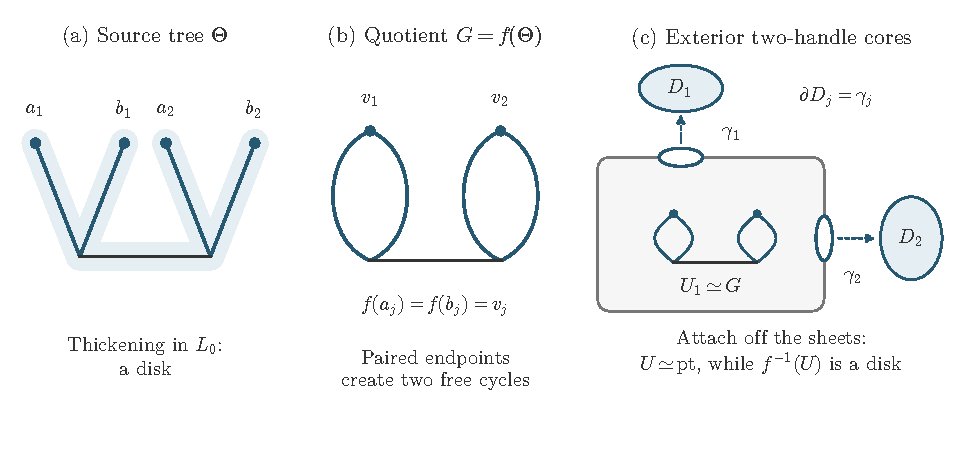
\includegraphics[width=\textwidth]{figures/topology-domain.pdf}
\caption{Source and target topology for two double points.
The source tree $\Theta$ joins the disjoint paths between paired
preimages $a_j,b_j$; its thickening is a disk.
Identifying each pair produces $G$, the spine of the zero- and
one-handlebody $U_1$.
Boundary circles $\gamma_j$ represent its free generators, and
exterior isotropic disks $D_j$ provide the cores of two-handles
that make $U$ contractible without changing its source preimage.
Panel~(c) records attachment data, not a planar embedding of disks
and sheets: the dashed arrows indicate attachments, the immersed
sheets are omitted, and the actual disk interiors lie outside
$U_1$ and avoid $f(L_0)$ in the $1028$-dimensional ambient manifold.}
\label{fig:topology-domain}
\end{figure}

\emph{Zero- and one-handles.}
Choose small disjoint radial Darboux balls at the vertices.  The
single sheet, or the pair of transverse Lagrangian sheets at a
double point, can be made linear in these coordinates.  For a pair,
straighten the first sheet, write the other as a gradient graph
over its transverse linear plane, and use the corresponding
symplectic shear to straighten it while fixing the first.  Arrange
the incident tree edges as distinct radial rays.  Join the balls
by sufficiently thin Weinstein one-handles along the remaining
edges, carrying strips of the corresponding sheets.

Here are explicit handle and attachment data, also fixing what
will be needed for two-handles.  In coordinates
$(u,v,z)\in\R^k\times\R^k\times\R^{2(n-k)}$, with form
$\sum du_j\wedge dv_j+\omega_z$, use the Liouville field
\begin{equation}\label{top:eq:handle-model}
       Z_k=-\sum u_j\partial_{u_j}
                    +2\sum v_j\partial_{v_j}
                    +\tfrac12\sum z_j\partial_{z_j},\qquad k=1,2.
\end{equation}
It has an index-$k$ quadratic Lyapunov function.  A thin handle box
has core $v=z=0$, negative face near $|u|=1$, and the remaining
faces positive after rounding.  For $k=1$, $v=0$ with $z$ in a
fixed Lagrangian plane is an invariant Lagrangian strip.

We require attachment maps strict for the selected contact forms,
not merely contactomorphisms of their kernels.  To obtain them,
choose near each attaching isotropic locus a slice transverse to
the Reeb field and tangent to the contact hyperplane along that
locus.  Reeb flow expresses the form as $da+\beta$ on a product
neighborhood of the slice, with $d\beta$ symplectic.  Match the
slices by the isotropic symplectic neighborhood theorem with the
chosen symplectic normal data.  The two resulting primitives differ
by a closed one-form restricting to zero on the isotropic locus.
A sufficiently small neighborhood retracts onto that locus, so
the difference is $dh$ with $h=0$ there.  A shift of the Reeb
coordinate by $h$, with the appropriate sign, makes the map
strict.  The same argument works for a Legendrian patch.
Extending by Liouville flow then gives collar identifications
preserving both the symplectic forms and their primitives.

Choose the strip framings along each source edge so that its two
ends give these Legendrian patch identifications.  The relative
Lagrangian neighborhood theorem extends the strip map to a
symplectic map of a thin handle, with the prescribed collar germs.
One can see its relative character directly: take tubular
coordinates agreeing with the germs, identify their linear
symplectic normal data, and apply the relative Moser argument,
with its vector field zero on a smaller end collar.  Shrinking
the finitely many handles makes them embedded and mutually
disjoint away from their prescribed attachments.  They meet no
other sheets, since $f^{-1}(G)=\Theta$.  Their model primitives
glue by the strict collars.

The resulting rounded zero- and one-handlebody $U_1$ retracts onto
$G$.  Its preimage thickens $\Theta$, hence is a disk.  The
Liouville field is tangent to all its immersed sheets: this holds
in the radial balls and in the strip model, and the attachment
maps preserve it.  Equivalently $f^*\lambda=0$ there.  It follows
that the boundary of the disk is Legendrian and has a positive
cylindrical collar.  Retain a smaller radial ball at the
single-sheet vertex.

\emph{Exterior filling disks with prescribed area.}
Represent a free basis of $\pi_1(U_1)$ by disjoint isotropic
circles $\gamma_j\subset\partial U_1$ avoiding the Legendrian
boundary of the source disk.  These exist by the subcritical
contact embedding theorem \cite[Theorem~12.4.1]{Top:EMbook}.
For circles the formal condition is just a nonzero tangent line
in the contact bundle; there is no extension obstruction, and
the dimensions permit disjointness and avoidance.  The dual
handle decomposition shows that
$\partial U_1\to U_1$ is an isomorphism on $\pi_1$, so these
circles may be chosen in the required free homotopy classes.

Join each $\gamma_j$ by an annulus in $U_1$ to the corresponding
graph cycle.  Both boundary integrals of $\lambda$ vanish:
one curve is contact-isotropic and the other lies on sheets with
zero primitive.  Stokes' theorem gives zero area for the
annulus.  Glue it to the chosen zero-area filling of that cycle.
This specifies a relative homotopy class of disks in $M$ with
boundary $\gamma_j$ and area zero.  Prescribe near the boundary
the outward Liouville-flow collar of $\gamma_j$; this collar is
isotropic and does not change that area.

Put $M_1=M\setminus\operatorname{int}U_1$.  Restoring $U_1$
from its boundary adds only handles of indices $2n-1$ and
$2n$.  Thus the inclusion $M_1\to M$ is an isomorphism on the
low relative homotopy problems in dimensions two and three.
In particular the specified disk classes, relative to their
boundary collars, have representatives in $M_1$.  Their areas
remain zero because the representatives are homotopic relative
to the boundary in $M$.  This is where retaining the filling
class is essential: $\pi_2(M)$ is not zero, and an arbitrary
exterior filling would not have the same area.
General position relative to the collars makes these smooth
disks embedded, pairwise disjoint, and disjoint from $f(L_0)$
off the prescribed domain attachments.  The relevant
inequalities are $2+2<2n$ and $2+n<2n$.

\emph{Making the disks isotropic.}
Take the prequantization circle bundle $Q\to M$ for the
integral form $\omega$, with connection form $\vartheta$
normalized by $d\vartheta=\pi_Q^*\omega$ and circle parameter
in $\R/\Z$.  It is a contact manifold.  Each prescribed
isotropic disk collar has a horizontal lift.  Over its smooth
filling disk trivialize the circle bundle and write the
connection as $d\theta+\beta$.  The horizontal boundary lift
has winding number
\begin{equation}\label{top:eq:zero-winding}
       -\int_{\partial D^2}\beta=-\int_{D^2}\omega=0.
\end{equation}
It therefore extends to a smooth lift of the whole disk,
relative to a smaller collar.  Exact zero area, rather than
area merely integral, is what ensures this relative extension.
The lifts are embedded and pairwise disjoint because the
underlying smooth disks are.

We check the complete formal isotropic condition.  Trivialize
the pulled-back contact bundle over a lifted disk and fix a
frame of its tangent bundle.  Ordered isotropic two-frames
retract to $U(n)/U(n-2)$, whose fundamental group vanishes.
Thus the prescribed isotropic derivative on the collar extends
to an isotropic monomorphism over the disk.  Its inclusion in
the ambient tangent bundle and the actual disk derivative are
homotopic relative to the collar: the real two-frame space
$V_2(\R^{2n+1})$ has vanishing $\pi_2$ (indeed it is
$(2n-2)$-connected).  This gives formal isotropic embeddings
of the disjoint union of disks with the fixed collar germs.
Since $2<n$, the relative $C^0$-dense subcritical contact
embedding theorem \cite[Theorem~12.4.1]{Top:EMbook} realizes
them by genuine isotropic embeddings.

Their projections to $M$ are isotropic immersions, because
$d\pi_Q$ identifies the contact hyperplane symplectically with
$TM$.  These projections may be made embedded and pairwise
disjoint while preserving all avoidance conditions.  To justify
the needed transversality within contact-isotropic maps, a
contact Hamiltonian $H$ gives a vector field satisfying
\[
 \vartheta(X_H)=H,\qquad
 \iota_{X_H}d\vartheta=(R_\vartheta H)\vartheta-dH.
\]
Prescribing $dH$ on the contact hyperplane at a point prescribes
an arbitrary projected velocity.  At distinct points of the
embedded lifted union these choices are independent by
disjointly supported Hamiltonians.  Relative transversality
therefore removes projected double points and intersections
between disks, of expected dimension $4-2n<0$, and intersections
with the immersed $L_0$, of expected dimension $2-n<0$.
Take all perturbations zero on a narrower collar.  Compactness,
the immersion property near the diagonal, and sufficiently
small perturbations away from that collar preserve exterior
placement and the prescribed attachments.  We have obtained
disjoint isotropic core disks in $M_1$.

\emph{Two-handles and contractibility.}
Attach thin index-two handles of \eqref{top:eq:handle-model}
along these core disks.  Choose the attaching parametrization
and the symplectic normal framing by restriction from the
actual core disk.  This removes any framing extension problem:
the tangent and normal data of the collar identification are
the restrictions of data already defined over the core.
The relative isotropic neighborhood theorem and relative
Moser argument embed the handles with those collar germs.
Their primitives glue by the strict collar construction above.
They miss the immersion, and sufficiently thin handles are
mutually disjoint.  Rounding the positive corners gives a
Weinstein domain $U$ with all the asserted primitive and
collar properties.

The domain retracts onto $G$ with one two-cell attached along
each free generator.  After contracting a maximal tree, this
is a bouquet of circles with its free basis killed by those
cells; its cellular complex is acyclic and its fundamental
group is trivial, so it is contractible.  No two-handle meets
the immersion, so the source preimage remains the disk
constructed in $U_1$.  The single-sheet radial ball also
remains unchanged.
\end{proof}

\subsection{Cancellation and the parity of double-point degrees}

\begin{lemma}\label{top:lem:odd-doubles}
The immersion may be replaced on the source disk of
Lemma~\ref{top:lem:exact-domain} so that every double point has
oriented intersection sign $(-1)^{n/2-1}$.  The replacement
preserves the integral grading, spin structure, pushed-forward
fundamental class, and the cohomology and homology maps in
\eqref{top:eq:source-properties}.
\end{lemma}

\begin{proof}
Complete $U$ at its positive boundary and extend the immersed
source disk by its positive cylinder.  Remove the center of
the single-sheet radial Darboux ball.  This creates a negative
Liouville end, whose Lagrangian asymptote is the standard
Legendrian link of a real plane.  The source is
$S^{n-1}\times\R$.  The punctured completion is simply
connected, since $U$ is contractible and $2n>2$.

Set $l=n/2$ and $m=|I|>0$.  We use the stabilization traces
of \cite[Lemma~3.2 and proof of Lemma~3.4]{Top:EEMS}.
The trace from a Legendrian link to its loose stabilization
has one double point of sign $(-1)^{l-1}$; the reversed
trace has sign $(-1)^l$.  Insert $m$ reverse traces in
separated collars near the negative end, running outward
from the $m$-fold stabilization to the original standard
link.  The negative link is now loose and the total signed
count is
\[
           I+m(-1)^l=0.
\]

The exact cancellation theorem of Eliashberg--Murphy
\cite[Theorem~2.3]{Top:EMcaps} applies with the following
verified hypotheses.  The target is a simply connected
Liouville manifold with a negative end.  The immersion is
proper, self-transverse, cylindrical at its negative end,
and has finitely many double points.  Its source is
connected.  Its primitive is exact because
$H^1(S^{n-1}\times\R;\R)=0$.  Its signed intersection
count is zero, and its single negative component is loose.
The additional infinite-width hypothesis in that theorem
is required only in dimension $n=3$, whereas here $n=514$.
The conclusion is a compactly supported Hamiltonian
regular homotopy to an embedding, leaving both tails
unchanged.

In the unchanged negative end, insert $m$ forward traces
from the original standard link to the $m$-fold
stabilization, and fill the center by the real plane.
All double points of the filled immersion are now the
$m$ double points of these traces, with sign
$(-1)^{l-1}$.  Its noncylindrical part is compact.  A
sufficiently long negative Liouville flow in the filled
positive completion moves this compact part into $U$.
The backward flow exists for all time: the compact domain
is backward invariant, and on the positive end the flow
translates the cylindrical coordinate.  Although it
rescales the symplectic form, it preserves Lagrangianity.
The positive cylinder is unchanged as a subset.  Trim at
its original boundary collar and glue to the unmodified
immersion outside the source disk.

The new source piece is a disk with the same collared
boundary.  A boundary identification extends to a
homeomorphism of the disks; under this comparison, the
two maps of the disk into $U$ are homotopic relative to
the boundary because $U$ is contractible.  Thus the
closed maps to $M$ have the same fundamental class and
induce the same maps on homology and cohomology.  This
argument uses contractibility of $U$, not asphericity of
$M$.  Orient the replacement compatibly.  Its spin
structure extends the old boundary spin structure,
since the sphere $S^{n-1}$ has a unique spin structure.
Every first homology class of the source can be
represented outside the replaced disk, so its Maslov
class remains zero.  The grading agrees on the common
complement after a constant shift, and then extends
over the replacement disk.
\end{proof}

For completeness, with the grading and orientation convention of
Section~\ref{sec:mirror}, transverse oriented graded Lagrangian
planes in complex dimension $2l$ satisfy
\begin{equation}\label{top:eq:parity}
       (-1)^{\deg(p_-,p_+)}=(-1)^l\operatorname{sign}(p).
\end{equation}
It follows either by rotating the first plane to the second in
diagonal unitary coordinates and counting the phase crossings,
or by the usual graded Euler-intersection formula.  Reversal of
the ordered pair changes its degree to $n-\deg(p_-,p_+)$,
so both ordered degrees have the same parity.  For the sign
in Lemma~\ref{top:lem:odd-doubles}, the right side of
\eqref{top:eq:parity} is $-1$.  Thus both degrees are odd.

\subsection{Rational areas and the fixed product labels}

\begin{lemma}\label{top:lem:rational-areas}
The immersion of Lemma~\ref{top:lem:odd-doubles} can be
perturbed arbitrarily slightly so that it has the incidence
properties and the common area denominator in
Proposition~\ref{prop:immersion}\textup{(iv)}, without changing
any of its other conclusions.
\end{lemma}

\begin{proof}
A generic small Hamiltonian perturbation gives
transversality to each of the finitely many product labels,
keeps its double values off those labels, and avoids their
pairwise intersections.  Indeed those intersections have
dimension strictly less than $n$, by the product-label
construction, so their intersection with a generic
$n$-dimensional immersed submanifold of $M^{2n}$ is empty.
There are now finitely many intersection points involving
the immersion, with distinct source preimages except for
the prescribed paired double preimages.

Restrict the prequantization bundle and connection to
$L$.  The connection is flat because $i^*\omega=0$.
Its holonomy on the torsion subgroup of $H_1(L;\Z)$
already has finite image.  On the free part, an arbitrarily
small closed one-form graph perturbation changes the
holonomy character by its period character.  Rational
characters are dense in this finite-dimensional character
torus, so choose such a perturbation to make the whole
holonomy finite.  A finite tensor power of the
prequantization bundle then has a parallel unit section
on $L$.  Choose a common power also supporting the
parallel sections on all the fixed labels.

For each double point, compare the values of the
parallel section at its two preimages.  For each
intersection with a label, compare the section on $L$
with the chosen section on that label.  Exact graph
perturbations by functions constant near the relevant
source points change these ratios by their endpoint
primitive differences while fixing the local sheets.
Because all the source patches can be chosen disjoint,
we can make the finitely many ratios roots of unity by
arbitrarily small such perturbations.  These exact
perturbations do not change the already finite holonomy.
They preserve transversality and create no new
intersections.  The comparisons between the fixed
labels are already roots of unity on every clean
component by Lemma~\ref{lem:rational-label-areas}.

Take a further common power killing all these roots of
unity.  The resulting parallel sections match at every
allowed boundary switch, including switches between
the two branches of the immersion.  For a disk with
such lifted boundary segments, parallel transport
therefore has holonomy one in that power.  The
curvature-holonomy formula gives
\[
                 \exp\left(2\pi\sqrt{-1}\,N_0
                         \int_{D^2}\omega\right)=1
\]
for one integer $N_0>0$ independent of the disk and its
number of corners.  Hence all these areas lie in
$N_0^{-1}\Z$.  Every perturbation used above is a
Lagrangian regular homotopy.  It preserves the spin
structure and grading, the parity of transverse
double points, the fundamental class, and the maps in
\eqref{top:eq:source-properties}.
\end{proof}

\begin{proof}[Proof of Proposition~\ref{prop:immersion}]
Start with Lemma~\ref{top:lem:source}, choosing the Euler
characteristic as in Lemma~\ref{top:lem:initial-immersion}.
Apply successively Lemmas~\ref{top:lem:zero-actions},
\ref{top:lem:exact-domain}, and \ref{top:lem:odd-doubles}.
Equation~\eqref{top:eq:parity} gives the required odd
corner degrees.  Finally apply
Lemma~\ref{top:lem:rational-areas}.  The fundamental
class, the degree-two quotient, and the homology
injection were established in
\eqref{top:eq:source-properties} and are preserved
at every subsequent step.
\end{proof}


\section{An immersed object detected by homology}
\label{sec:floer}

The construction of Section~\ref{sec:topology} controls the second Betti
number of a Lagrangian immersion.  To use that control on the mirror, we
need an uncurved object whose degree-two endomorphisms have no additional
generators at the double points.  This section proves the required
statement.  Its geometric ingredient is the interior-mark obstruction
argument of Fukaya--Oh--Ohta--Ono.  We extend that argument to an immersion
whose double-point degrees are odd, retaining all switching-node faces.
We then pass from solutions at finite energy cuts to an ordinary
$A_\infty$ category over an enlarged field.

\subsection{Coefficients, gradings, and finite constructions}
\label{subsec:floer-foundations}

We use the Novikov field
\[
 \Lambda=\left\{\sum_{j\geq0}a_jT^{\lambda_j}:
 a_j\in\C,\ \lambda_j\in\R,\
 \#\{j:\lambda_j\leq E\}<\infty\text{ for every }E\in\R\right\}.
\]
Terms with equal exponents are combined.  Write $v$ for the least exponent
of a nonzero series, $v(0)=+\infty$, and put
$\Lambda_0=\{v\geq0\}$ and $\Lambda_+=\{v>0\}$.
The exponent records symplectic area and has degree zero.  Algebraic
closure and the size of this field are recalled below.

Let $(X,\omega)$ be a closed symplectic manifold of real dimension $2n$,
equipped with a homotopy class of trivializations of its canonical complex
line bundle.  All Lagrangian branes considered here are compact,
integrally graded, and spin; the background class is zero.  A finite
collection is called clean when every pairwise fiber product of its
immersions, including a self-fiber product, is clean.  On a connected
component $R$ of such a fiber product, Floer cochains are differential
forms with the determinant orientation local system and the Maslov
degree shift.  Thus the underlying complex at energy zero is a direct
sum of shifted de Rham complexes.  The coefficients are extended from
$\R$ to $\C$ separately at each energy.

We use suspended $A_\infty$ signs.  If $|x|'=|x|-1$, the identities read
\begin{equation}
 \label{eq:floer-ainfinity}
 \sum_{s=0}^k\ \sum_{i=1}^{k-s+1}
 (-1)^{\sum_{j<i}|x_j|'}
 m_{k-s+1}(x_1,\ldots,x_{i-1},m_s(x_i,\ldots,x_{i+s-1}),
 x_{i+s},\ldots,x_k)=0.
\end{equation}
Here $m_k$ has ordinary degree $2-k$, and $m_{1,0}=d$.
The order of inputs follows the boundary order.  Composition in the
cohomology category includes the corresponding suspension sign.

We specify the foundational results used in the argument, and then
explain the finite-cut convention needed when constant polygons switch
branches.  The disk and strip construction of
\cite[Chapters~7--8]{Floer:FOOO}, its immersed extension
\cite[Sections~4--12]{Floer:AJ}, and the clean de Rham construction
\cite[Section~3]{Floer:Fukaya} provide the following ingredients:
\begin{enumerate}[label=(\roman*)]
 \item Fredholm charts obtained by adding finite-dimensional obstruction
 spaces supported in component cores, with auxiliary markings and
 transverse incidence conditions to stabilize the domains;
 \item gluing and coordinate changes compatible with normalization of
 boundary corners, where the obstruction spaces on a broken curve are
 sums of the spaces on its components;
 \item orientations from the spin structures and the determinant lines
 at the ends;
 \item extension, after thickening and outer collaring, of compatible
 CF-perturbations prescribed on normalized corners, with strong
 submersivity at the outgoing boundary evaluation;
 \item signed integration along the fiber, its Stokes formula and its
 composition formula, and relative versions over a parameter interval;
 \item the filtered construction and comparison theorem, including
 canonical models, passage from finite approximations to a filtered
 structure up to homotopy, and comparison of choices.
\end{enumerate}
For the clean disk charts and perturbations, precise statements are
\cite[Theorem~3.24 and Propositions~3.29--3.30]{Floer:Fukaya}.
The abstract extension and integration statements are those of
\cite[Chapters~9--10, 15, 17, and~21]{Floer:Kuranishi}.
The construction by core obstruction data, including its relative
and componentwise forms, is developed in
\cite{Floer:DisksI,Floer:DisksII}; smooth gluing coordinates are understood
with the correction in \cite{Floer:Corrigendum}.
We invoke these statements for the ordinary rooted disk problems.
The interior-rooted problems used below are constructed separately in
Lemma~\ref{lem:interior-construction}.

\begin{lemma}[Finite clean models]
 \label{lem:finite-clean-models}
For a finite clean collection of branes, the disk construction gives a
unital curved filtered $A_\infty$ category over $\Lambda_0$, with
finite-rank canonical morphism models.  The energy-zero differential on
the de Rham model is the ordinary differential on its sectors, and the
canonical model has those sectors' cohomology as its underlying graded
space.  Choices, restrictions to subcollections, and finite geometric
constructions compare by filtered homotopy equivalences through any
prescribed finite energy and arity cut.

All these structures and comparisons respect the integral grading.
For a self-transverse immersion $i:L\to X$ with only double points, its
canonical self space is
\begin{equation}
 \label{eq:floer-self-space}
 C^*(L,L)=H^*(L;\C)\otimes\Lambda_0
 \ \oplus\!\bigoplus_{(p,q)\in R_L}
 \ell_{pq}\otimes\Lambda_0,
\end{equation}
where $R_L=\{(p,q):p\ne q,\ i(p)=i(q)\}$, and $\ell_{pq}$ is a
one-dimensional line placed in the intersection degree $d(p,q)$.
For an embedded brane transverse to $i$ and avoiding its double values,
the mixed canonical spaces are the usual graded intersection lines.
\end{lemma}

\begin{proof}
The existence and comparison assertions are the filtered construction
theorems just listed.  We check the cutoff and grading issues relevant to
their use here.

At a fixed finite cut, let $\delta>0$ be a lower bound for positive
component energies.  Such a bound follows from disk compactness and the
energy gap for the finite list.  Choose $0<\varepsilon<\delta$ and assign
to an ordinary vertex of energy $E$ and arity $k$ the cost
\begin{equation}
 \label{eq:floer-cost}
 c(E,k)=E+\varepsilon(k-1).
\end{equation}
Costs add under tree substitution.  Every positive-energy zero-input
vertex has positive cost, as does every zero-energy stable vertex of
arity at least two.  The zero-energy unary operation is the fixed
differential and is handled algebraically.  A nontrivial breaking
therefore has lower-cost components.  An energy and arity bound gives
a finite collection of necessary moduli problems and their boundary
types: energy bounds control nonconstant components, stability and the
arity bound control constant components, and compactness gives finitely
many represented classes and charts.  In particular, we never bound the
number of switches in a constant polygon by its energy alone.

This is the geometric version of the finite $A_{n,K}$, or $A_{N,0}$,
construction.  One applies the relative extension theorem at successive
costs, including the necessary faces and homotopies.  Forgetful-map
conditions giving units reduce arity and fit the same induction.
Interval versions supply comparisons on common cuts.  The filtered
lifting theorem then produces a fixed model equivalent to each finite
construction through its cut; see
\cite[Sections~7--11]{Floer:AJ}.  This conclusion does not require one
transverse perturbation to work simultaneously at all energies.  If
the relevant energies lie in $\delta\Z$, one may choose
$\varepsilon=\delta/4$; the cost induction is then literally a discrete
induction.  More generally one uses the gapped energy set and the
equivalent finite energy--arity ordering.

For the grading, cap each transverse end by a path lifted according to
the brane grading.  The determinant trivialization and the grading make
the closed capped Maslov contribution zero.  The sphere contribution is
also zero because the first Chern class vanishes.  Fredholm indices
therefore give the integer degree $2-k$ for $m_k$, with $T^E$ of degree
zero.  At a clean component the same index formula includes the ordinary
form degree and the constant Maslov shift.  Reversing a clean component
of dimension $r$ changes its shift to the complementary shift whose sum
with the original is $n-r$.  Thus evaluation pushforwards and matching
at nodes preserve the integer degree, not just its parity.  A
Hamiltonian isotopy transports the lifted capping paths.

At energy zero a unary stable nonconstant map cannot occur, and a
constant strip with transverse ends contributes no differential on a
point sector.  The remaining unary operator is $d$.  Transfer with
respect to this differential gives the displayed finite-dimensional
cohomology spaces.  The unit can be retained in this transfer by choosing
the contraction to fix the constant function.  On transverse mixed
sectors there is nothing to transfer.  These observations prove
\eqref{eq:floer-self-space} and the assertion about mixed spaces.
\end{proof}

A cochain $b$ of ordinary degree one and positive valuation twists the
operations by inserting arbitrarily many copies of $b$ in all gaps.
The sums converge: an insertion contributes a uniformly positive amount
to the valuation for each fixed cochain.  Write
\[
 \Delta(b)=\sum_{k\geq0}m_k(b,\ldots,b).
\]
The equation $\Delta(b)=0$ is the zero-curvature Maurer--Cartan equation.
We use this equation, rather than the weaker equation permitting a
multiple of the unit.

\subsection{The statement for an immersed brane}

\begin{proposition}[An immersed object with homological detection]
 \label{prop:immersed-package}
Let $(X^{2n},\omega)$ and a finite clean collection be as above, with
$n$ even.  Fix a compatible almost complex structure $J$ admitting no
nonconstant $J$-holomorphic sphere.  Suppose a label $i:L\to X$ satisfies:
\begin{enumerate}[label=(\alph*)]
 \item its self-intersections are transverse double points, and both
 ordered intersection degrees at each double point are odd;
 \item the map
 $i_*:H_{n-2}(L;\Q)\longrightarrow H_{n-2}(X;\Q)$ is injective;
 \item areas of the self-disk problems for $L$, including polygons with
 switches, belong to a locally finite additive submonoid
 $G\subset\R_{\geq0}$.
\end{enumerate}
Fix positive-valuation zero-curvature bounding cochains on any selected
other labels.  There is an algebraically closed field $\kappa$ containing
$\Lambda$, of cardinality at most continuum, and a unital uncurved
$\kappa$-linear $A_\infty$ category containing those bounded labels and
a new object, denoted $\mathbf L$, with the following properties.
\begin{enumerate}[label=(\roman*)]
 \item The full category on the other bounded labels is the scalar
 extension of their original category.
 \item $\dim_\kappa H^2\Hom(\mathbf L,\mathbf L)\leq b_2(L)$.
 \item If $D$ is one of the selected bounded labels, is embedded,
 and is transverse to $i$ and avoids its
 double values, the underlying mixed spaces involving $D$ and
 $\mathbf L$ are the graded intersection lines for $D$ and $i$.
 \item If, in addition, $D$ is connected and its bounded self-Floer
 cohomology has the full graded dimensions of $H^*(D)$, composition
 followed by its top trace gives perfect pairings
 \[
 H^p\Hom(D,\mathbf L)\otimes
 H^{n-p}\Hom(\mathbf L,D)\longrightarrow\kappa
 \qquad(p\in\Z).
 \]
\end{enumerate}
The trace in (iv) is nonzero on the one-dimensional top self-Hom of
$D$.  The proposition asserts an ordinary object over $\kappa$; it does
not assert that $L$ has a bounding cochain in the original Novikov field.
\end{proposition}

Here locally finite means that $G\cap[0,E]$ is finite for every $E$.
Fix $\delta>0$ with $G\cap(0,\delta)=\varnothing$; if $G=\{0\}$,
any positive $\delta$ will do.  All comparisons used for the self-label
keep $J$ and the immersion fixed, so their energy indices belong to
$G$.  The discrete rational-area condition supplied by
Proposition~\ref{prop:immersion} is a special case.

The proof has three steps.  We first construct the interior-mark
operations needed to detect the first surviving curvature coefficient.
We then remove curvature at any finite energy cut in the geometric
model.  Finally we transport these approximate solutions to one fixed
finite model and pass to a residue field.

\subsection{An interior mark and its boundary strata}
\label{subsec:interior-mark}

For the remainder of the geometric argument, use the single immersion
$i:L\to X$.  Its diagonal sector is $\Omega^*(L;\C)$; a switch sector is
the shifted point line $\ell_{pq}$.  Ordinary disk operations have a
distinguished boundary output.  We also consider stable disks with one
interior marked point, $k$ cyclically ordered boundary inputs, and no
distinguished boundary output.  The boundary lift to $L$ is continuous
between designated switches.  The word ``cyclically'' specifies the
action relabeling the $k$ boundary inputs; integrations take place on
the labeled spaces, without dividing by this action.

For $\eta\in\Omega^*(X;\C)$, pull back $\eta$ by the interior evaluation
and integrate it together with the boundary inputs.  The resulting
scalar operation is written $p^\eta_k$.  Its terms carry their area
weights.  A stable constant disk with one boundary input and the
interior mark is included.  The constant problem with no boundary input
is unstable and is not included.

On a component with continuous boundary lift the Maslov index is zero.
The real map index is therefore $n$.  Subtracting the three disk
automorphism parameters and adding the marked-point parameters gives
virtual dimension $n+k-2$ for $k$ inputs and a boundary output, and
$n+k-1$ for $k$ boundary inputs and the interior mark.  These are the
dimension formulas used below.

\begin{lemma}[Finite interior-mark construction]
 \label{lem:interior-construction}
Fix the ordinary rooted disk data through a finite energy--arity cut,
enlarged to include all factors of the required boundary strata.
The preceding interior-mark spaces admit oriented Kuranishi structures
and CF-perturbations relative to those data, with the following features:
\begin{enumerate}[label=(\roman*)]
 \item Every boundary product is rooted at the component carrying the
 interior mark.  Its other vertices carry the ordinary rooted disk
 data.  Both diagonal matching nodes and inverse switching nodes are
 included.
 \item The additional interior evaluation is strongly smooth.  No
 submersivity is required of it.  At a diagonal matching node the
 ordinary child evaluation is strongly submersive for the
 CF-perturbation.
 \item The interior-rooted data are equivariant under cyclic relabeling
 of their external boundary inputs, with the determinant orientation
 signs.  The ordinary rooted child data need not be cyclic.
 \item The integrations obey Stokes and composition on these boundary
 products.  At energy zero,
 \begin{equation}
  \label{eq:floer-p-leading}
  p^\eta_{1,0}(x)=\pm\int_L i^*\eta\wedge x
 \end{equation}
 on closed forms.  The sign is fixed and nonzero.
\end{enumerate}
\end{lemma}

\begin{proof}
We construct the interior-rooted spaces with all immersed boundary
labels.  Their local boundary problems are the ordinary diagonal and
transverse-jump problems of \cite[Sections~4--5]{Floer:AJ}; the
relative construction below specifies their organization when no
boundary output is chosen.  It uses the mixed parent--child
organization of \cite[Propositions~16.3 and~16.14]{Floer:AFOOO2026}, retaining
reciprocal internal switches even when the external word is empty.
The parent is always additional interior-rooted data.  Its
identification with a boundary-rooted bulk operation is neither
required nor imposed.

\emph{Compactification and normalization.}
Keep the interior mark in immersed stable-map compactness.  At a
boundary node the two lifts either agree in $L$ or end at distinct
preimages $p,q$ of a double value.  In the latter case the two
normalized flags have the reciprocal labels $(p,q)$ and $(q,p)$.
These flags disappear from the external word on gluing; they remain
part of the normalized stratum.  In particular, an empty external
word does not restrict its compactification to the diagonal sector.

There are no nonconstant spheres.  A connected tree of constant
spheres attached at one interior node and carrying at most the one
interior mark cannot be stable: it has fewer than three external
special points in total.  The degeneration in which the entire
boundary collapses would retain a nonconstant sphere, and is also
absent.  All remaining strata are disk trees.  Constant stable
vertices are retained, including the disk with the interior mark
and one boundary node.  The constant disk with no boundary input or
node and only the interior mark is unstable and gives no stratum.

Let $v_*$ be the vertex carrying the interior mark.  Orient every
edge toward $v_*$.  A vertex other than $v_*$ then has exactly one
outgoing flag, which is its ordinary disk output; every remaining
flag is an input.  A normalized corner is the product of the moduli
problems on these vertices, with the diagonal matching equations
and reciprocal-label matches along its edges.  For any collection
of edges, cutting them in any order produces this same oriented
tree and the same factors.  The root of each separated component
is either $v_*$ or its unique edge toward $v_*$.  This rule also
describes intermediate faces, so the identifications on iterated
normalized corners agree.

Stabilization respects these identifications.  Forgetting auxiliary
marks contracts only constant unstable components.  Contracting a
non-root such component carries the unique path toward $v_*$ to the
unique path toward $v_*$; hence the output flag on every surviving
ordinary component is unchanged.  A constant component carrying the
interior mark and an attaching boundary node is stable and cannot
be contracted.  If it has no such node, it is the excluded constant
zero-input root.  An unstable constant bivalent disk has either two
diagonal nodes on the same sheet or two reciprocal switch nodes:
its two constant boundary arcs rule out exactly one switch.  Its
contraction preserves the labels of the surviving flags.  The
two-switch constant strip is the identity under the dual cap-line
identification fixed by determinant gluing; it is not a new
orientation choice \cite[Sections~4.3 and~5]{Floer:AJ}.
Thus a contraction performs the same pairing
of the ordered cap lines whichever order of normalization is used.
For a chain of these components, the neck lengths concatenate as
$T=T_1+\cdots+T_j$.  This is associative.  Forgetting is interpreted
in the admissible category of \cite[Section~14.3]{Floer:AFOOO2026}:
its pullbacks of admissible obstruction and CF data are admissible
and smooth in the gluing profiles used for integration.  The
forgetting map itself need not be smooth in ordinary corner
coordinates.  This admissible compatibility gives compatibility
with stabilization as well as with cutting a fixed tree.

These constructions are equivariant under isomorphisms of decorated
trees.  Such an isomorphism fixes the interior mark and preserves
the directed paths to it, so it never changes an ordinary child's
output.  Relabeling external inputs permutes their positions without
rerooting any ordinary child.  The same statement holds for an
automorphism permuting several isomorphic subtrees.  Normalized
corners retain their ordering of the cut edges; changing that
ordering permutes the outward normal lines with their determinant
sign.  Their subsequent finite quotients therefore have the required
corner identifications and automorphism weights.

\emph{Relative charts and smoothing.}
At a smooth nonconstant root choose auxiliary marked points on
compact cores, in free orbits of its finite automorphism group,
and impose transverse incidence conditions.  Choose obstruction
sections supported away from the distinguished mark, the nodes,
and the strip ends.  Their span can make the augmented
Cauchy--Riemann operator surjective: a cokernel vector annihilating
all such sections would vanish on an open core and then vanish by
unique continuation.  Taking the span of the stabilizer translates
makes this an invariant finite-dimensional obstruction space.
If effective charts are used, include vectors $D_u\xi$ for map
variations $\xi$ supported on disjoint free stabilizer-orbit balls
in the core.  These variations lie in the augmented kernel and
carry a faithful stabilizer representation modulo infinitesimal
reparametrizations; they make the thickened chart effective.
No submersivity is requested at the interior evaluation, which is
used only to pull back $\eta$.

At a broken root use the direct sum of the obstruction data on its
normalized components.  Ordinary vertices carry the fixed ordinary
data.  At a diagonal edge the child output evaluation is submersive,
so component surjectivity remains surjectivity after imposing the
matching equation in $L$.  All matching equations can be solved
recursively from the root toward the leaves: having chosen the
parent variation, choose the child's variation with the required
output value and continue with its children.  Joint submersivity
of all boundary evaluations on one component is not needed.
At a reciprocal switch the matching
space is a point; the operator has precisely the transverse
fixed-jump asymptotic condition of the immersed disk charts.
The linear and nonlinear gluing problems are therefore those of
the ordinary immersed construction, with the interior-mark
coordinate added on the root component.  A constant root
stabilized by that mark is kept as a marked component in this
description.

Transport obstruction sections from the compact cores into the
plumbed domains.  Exponential gluing estimates give charts through
the smoothing parameters, with the corrected smooth gluing
profiles cited above.  Coordinate changes are obtained from
componentwise obstruction data.  We specify their relative choice,
so that compatibility is more than a choice of unrelated local
thickenings.  Use the quasi-component construction of
\cite[Conditions~8.12--8.15, Lemmas~8.19--8.20, and
Definition~8.21]{Floer:DisksII}.  A quasi-component records a
transported compact-core obstruction choice and its auxiliary
stabilization data.  On a boundary tree take the componentwise
union of the already chosen indices: those of its interior root
and the fixed indices of its ordinary vertices.  The directed-tree
identifications show that this prescription agrees on every
iterated boundary and stabilizer quotient.

Extend the corresponding open family of indices inside a proper
family over a sufficiently small boundary neighborhood, as in
\cite[Proposition~8.18]{Floer:DisksII}.  Complete its finite cover
by new compact-core choices on the root away from a smaller
neighborhood, and saturate the choices under the finite
automorphism groups.  Choose the new compact-core spaces generically
transverse to the finitely many inherited spaces and their
stabilizer translates, as in the quasi-component construction.
Surjectivity and these direct-sum conditions are then open;
shrinking the neighborhoods preserves them.
Properness gives the semicontinuity inclusion of obstruction
spaces under changes of the central map, as in
\cite[Proposition~8.17]{Floer:DisksII}.  These inclusions and
forgetting the auxiliary marks define the coordinate changes;
they satisfy the cocycle conditions because the index inclusions
compose and the admissible forgetting operations commute with
normalization.  The original boundary families are unchanged on
the smaller collar.  This is the componentwise proof of
\cite[Theorems~5.3 and~5.4]{Floer:DisksII}, with its additional root
data specified relatively.  The local diagonal and fixed-jump
operators and the augmented matching surjectivity verified above
are exactly what that construction uses.  The fixed ordinary
factors are retained.

\emph{Finite extension of perturbations.}
Let $\delta>0$ be a lower bound for positive component energies,
and choose $0<\varepsilon<\delta$.  Assign cost
$E+\varepsilon(k-1)$ to an ordinary vertex of energy $E$ with $k$
inputs and cost $E+\varepsilon k$ to an interior-rooted vertex.
These costs add under boundary splitting.  Every ordinary stable
vertex has positive cost: the zero-energy unary strip is unstable
and represents the separately fixed de Rham differential, and a
zero-energy stable ordinary vertex has at least two inputs.  The
constant one-input interior root has cost $\varepsilon$; the
constant zero-input root is excluded.  Each nontrivial breaking
therefore has lower-cost factors.  The locally finite energy set,
the arity cutoff, and stability give a finite collection of
problems and normalized corner types, after adjoining all required
faces.  This includes constant switching polygons; their number of
inputs is controlled by arity, not by their zero energy.

Induct on this finite order.  On every normalized boundary prescribe
the product of the already constructed interior-rooted parent
perturbation and the fixed ordinary child perturbation.  The
prescriptions agree on higher corners by the directed-tree and
stabilization identifications.  Diagonal fiber products are defined
because the child output is strongly submersive for its fixed
CF-perturbation; reciprocal switches are products over points.
First extend these compatible normalized-boundary products to a
corner neighborhood by outer collaring, as in the collar step of
\cite[Proposition~14.8 and Remark~14.7]{Floer:AFOOO2026}.  The required
agreement on iterated normalized boundaries is precisely the
agreement verified above, including their stabilizer quotients.
Apply \cite[Proposition~14.5]{Floer:AFOOO2026} with the map to a point
and with the closed smaller corner neighborhood as its prescribed
set.  It supplies a compatible thickening and extends the
CF-perturbation over the new root space while retaining it near
that set.  Composition on the prescribed collar still uses the
original ordinary child perturbations.  There is no requirement
to forget a boundary input on the new root space and no new
submersion condition at its interior mark.

For cyclic relabeling and finite stabilizers, take invariant
obstruction spaces and include the finite-group representations in
the auxiliary parameter spaces of the CF-perturbations.  The
prescribed corner products are equivariant, so the same relative
extension is equivariant.  This uses equivariant families, not
single-valued equivariant transverse sections.  Finite quotients
are integrated with their ordinary stabilizer weights.  Stokes and
composition now apply to every prescribed product.  The identical
construction over a parameter interval, relative to its endpoints,
supplies finite-cut comparisons whenever the ordinary choices vary.

\emph{Orientations and the zero-input identity.}
Use the spin determinant orientations and the graded cap lines at
all transverse flags, with the local normalization specified below.
At a reciprocal node the two cap lines are paired in their ordered duality; at a diagonal node they are
replaced by the matching determinant of $TL$.  Determinant gluing
is associative.  Permuting normalized smoothing normals or cap
lines gives exactly their Koszul signs, including at an
automorphism quotient.  Stabilizing marks together with their
incidence constraints contribute canceling orientation factors.
These are the orientation conventions for ordinary immersed disk
composition; adding the even-dimensional interior-mark coordinate
does not alter its cap-line rule.

For $k=0$, pull back the closed $(n-2)$-form $\eta$ to the virtual
$(n-1)$-space.  Each boundary product has a single ordinary
curvature child and an interior-rooted parent with one input.
Composition first identifies its contribution with
$p_1^\eta(m_0)$, with the common Stokes sign.  This includes every
reciprocal-switch product.  Only after composition do we use the
grading: a curvature output has degree two, while each branch
generator has odd degree, so those child outputs vanish.
There is no sphere or boundary-collapse term.  Stokes therefore gives
$p_1^\eta(m_0)=0$ for closed $\eta$ of degree $n-2$.

At energy zero the one-input diagonal root is the regular constant
disk space $L$.  Its one boundary mark and one interior mark fix
the domain; its evaluations are the identity and $i$.  Integrating
a boundary form gives
\eqref{eq:floer-p-leading}, with the fixed orientation sign.  The
boundary-rooted operations were never changed in this construction.
\end{proof}

\subsection{The signed obstruction identity}

We record the signs because the obstruction argument uses the sum over
all cyclic positions, including its two extreme cases.  On the
diagonal sector the spin cappings are the ordinary embedded-disk
cappings.  The local orientation calculation at a diagonal node is
therefore the embedded calculation, even if the moduli space has
switching-node strata elsewhere.

Here is an explicit normalization of that calculation.  Put the
output test form first, followed by the boundary input forms, in the
geometric integral.  Write $X_0$ for the degree of the output test
form; in the interior-rooted case this form is $\eta$.
At a smooth boundary slot of degree $X_j$, the
signed boundary-rooted and interior-rooted operations have exponent
\begin{equation}
 \label{eq:floer-p-sign}
 \sum_{j=1}^k jX_j+\binom{k-1}{2}+\epsilon_0,
\end{equation}
where $\epsilon_0$ is the one fixed bare smooth-node gluing sign.  The
binomial coefficient has its polynomial meaning also at $k=0$.
This is a choice of the signed $m,p$ conventions together; the unstable
unary operation is $m_{1,0}=d$.  Reversing all boundary conventions
replaces both operations by their $A_\infty$ opposites and gives the
same conclusions.

For clarity, one can verify the normalization as follows.  In the
determinant line order put the capped disk operator and inverse disk
automorphism orientation first, then the marked-point tangent factors
in boundary order.  The former combined factor has odd parity when
$n$ is even, each smooth boundary mark has odd parity, and the interior
mark has even parity.  Consider a child containing $s$ consecutive
inputs starting at position $i$, with $r=k-i-s+1$ trailing inputs.
Put parent before child in the product orientation.  Moving the child
block through the trailing factors, with outward normal first, gives
the bare boundary exponents
\begin{equation}
 \label{eq:floer-boundary-signs}
 i+sr+\epsilon_0
 \quad\hbox{for a boundary-rooted parent},\qquad
 i-1+sr+\epsilon_0
 \quad\hbox{for an interior-rooted parent}.
\end{equation}
The tangent of the diagonal matching copy of $L$ has even dimension
and contributes no further parity.  The difference of one in these
two formulas is precisely the change from the odd boundary-output
tangent factor to the even interior-mark factor.

Let $X_z$ be the ordinary degree of the child output form.  Its degree
formula gives $X_z=\sum_{\rm child}X_j+2-s$.  In the Fubini comparison,
moving child inputs past trailing inputs and then moving their output
back into the node slot contributes
$F=(\sum_{\rm child}X_j+X_z)\sum_{\rm trailing}X_j$.
Let $A_k$ be the exponent in \eqref{eq:floer-p-sign} for the original
input word, and let $A_P,A_C$ be the corresponding parent and child
exponents, with $X_z$ in the parent node slot.  Put
$I=\sum_{j<i}(X_j-1)$, and denote the appropriate bare exponent in
\eqref{eq:floer-boundary-signs} by $B$.  Direct substitution gives
\[
 A_k+A_P+A_C+B+F\equiv
 \begin{cases}
 I+\sum_jX_j+k+1,&\text{boundary output},\\
 I+\sum_jX_j+k,&\text{interior output}
 \end{cases}
 \pmod2.
\]
After the input degrees have canceled, the constant part of this
calculation is the identity
\[
 k+s(k-s+1)+\binom{k-1}{2}+\binom{k-s}{2}
                   +\binom{s-1}{2}=0\pmod2.
\]
This polynomial identity also covers $s=0$ and $s=k$.
For Stokes with a boundary output, the parity condition for the
integrated form is $X_0+\sum X_j=k+1$ modulo two; with an interior
output it is $X_0+\sum X_j=k$ modulo two.  Thus in both cases the
displayed exponent is $I+X_0$.

Write the raw Stokes equation as
$\int_{\partial\mathcal M}\Omega-\int_{\mathcal M}d\Omega=0$,
where $\Omega$ is the product of the test form and input forms.
Multiply this whole equation by $(-1)^{A_k+X_0}$.  After rewriting
a boundary product in the signed operations, its exponent is
$A_k+X_0+A_P+A_C+B+F\equiv I$, as required.
For the differential of the $i$th input, the raw exterior-derivative
sign is $X_0+\sum_{j<i}X_j$, and the minus sign in the Stokes
equation contributes one.  The operation with that differentiated
input has exponent $A_k+i$.  Its normalized exponent is therefore
\[
 (A_k+X_0)+1+X_0+\sum_{j<i}X_j+(A_k+i)
 \equiv\sum_{j<i}(X_j-1)\pmod2.
\]
This gives the same insertion sign and accounts for $m_{1,0}=d$.
Thus the interior Stokes formula has the suspended insertion signs
of \eqref{eq:floer-ainfinity}, and no output differential when $\eta$
is closed.  This is the $\mathfrak p$ convention of
\cite[Section~3.8]{Floer:FOOO}; the calculation is also the pure-sector
normalization in \cite[Section~6]{W}.

A cyclic move of the first boundary input to the last has sign
\begin{equation}
 \label{eq:floer-cyclic-sign}
 (-1)^{(X_1-1)\sum_{j>1}(X_j-1)}.
\end{equation}
Indeed the boundary tangents contribute $k-1$.  Permuting the input
forms contributes $X_1\sum_{j>1}X_j$, and changing
\eqref{eq:floer-p-sign} contributes
$(k-1)X_1+\sum_{j>1}X_j$.  Their sum is the exponent displayed above.
These determinant computations also hold on the thickened charts:
obstruction directions and their duals are inserted compatibly with
gluing, and adding stabilization marks together with incidence
constraints inserts canceling orientation factors.

\begin{lemma}[Interior obstruction identity]
 \label{lem:interior-identity}
Assume the hypotheses on $L$ in Proposition~\ref{prop:immersed-package}.
Let $b$ be a positive-valuation degree-one cochain supported on the
diagonal de Rham sector.  At any finite cut at which the expressions are
defined, and for every closed $\eta\in\Omega^{n-2}(X;\C)$,
\begin{equation}
 \label{eq:floer-interior-identity}
 \sum_{r\geq0}p^\eta_{r+1}(\Delta(b),b,\ldots,b)=0
\end{equation}
through that cut.  The curvature $\Delta(b)$ is supported on the
diagonal sector and has ordinary degree two.
\end{lemma}

\begin{proof}
Every $m_k(b,\ldots,b)$ has degree two.  A switch sector is a point
line of odd degree and has no degree-two cochain.  Hence the curvature
has no switch component.  In the boundary formula for an
interior-rooted disk with diagonal inputs, a child whose output is a
switch similarly pushes forward to zero: its required output degree
would be two on that shifted point.  We include these faces in the
geometric construction and use this degree calculation only after
taking their child pushforwards.  Composition of correspondences then
makes their entire contributions zero.

All remaining faces have a diagonal child output.  Their signs are the
ones calculated above.  Apply Stokes to the interior-rooted spaces
with $k>0$ copies of $b$, and divide the resulting equation by $k$.
A child carrying a block of $s$ external inputs has $k$ cyclic
placements.  For $0<s<k$ these are the starts of the block.  For $s=0$
they are the $k$ cyclic gaps.  For $s=k$ the child carries all inputs,
and its output node occupies one of the $k$ gaps, giving the $k$
possible rooted linear orders on that child.  Input differentials
likewise occur in $k$ positions.  Since $b$ has suspended degree zero,
moving the curvature input back to the first parent slot gives no
sign by \eqref{eq:floer-cyclic-sign}.  The normalized contribution is
therefore
\[
 \sum_{r+s=k}p^\eta_{r+1}(m_s(b,\ldots,b),b,\ldots,b),
\]
with the differential included in $m_1$.

For $k=0$ the boundary is a single curvature child attached to the
interior-rooted parent, including the stable constant one-input
parent.  Its contribution is $p^\eta_1(m_0)$.  There is no unstable
constant $p_0$ contribution, and no collapsed-boundary sphere term by
Lemma~\ref{lem:interior-construction}.  Summing over $k$ proves
\eqref{eq:floer-interior-identity}.  The sum is finite through the
chosen cut because $b$ has positive valuation.  All divisions take
place in characteristic zero.
\end{proof}

\subsection{Removing curvature through a finite cut}

\begin{lemma}[Approximate bounding cochains]
 \label{lem:approximate-bounding}
Under the hypotheses of Proposition~\ref{prop:immersed-package}, for
every $E>0$ there is a finite geometric construction and a diagonal
degree-one cochain $b_E$ with $v(b_E)\geq\delta$ such that
$v(\Delta(b_E))>E$.  These solutions can be transported to a fixed
finite-rank curved model, giving degree-one cochains $\widetilde b_E$
with a common positive valuation lower bound and with curvature
valuations tending to infinity.
\end{lemma}

\begin{proof}
Work first with an energy cut high enough for all operations about to
be used.  Start with $b=0$.  Suppose the coefficients of $\Delta(b)$
below $\lambda\in G\setminus\{0\}$ vanish, and let $o_\lambda$ be its
coefficient at $T^\lambda$.  The curved $A_\infty$ equation, evaluated
on $b$, says
\[
 \sum_{r,t\geq0}
 m_{r+1+t}(b^{\otimes r},\Delta(b),b^{\otimes t})=0.
\]
At energy $\lambda$ only the zero-energy unary term acts on
$o_\lambda$: every other displayed term contains either positive
operation energy or an additional $b$ input.  Consequently
$d o_\lambda=0$.

Apply Lemma~\ref{lem:interior-identity}.  At the same energy, the only
surviving term is the zero-energy $p_1$ term on $o_\lambda$.  Thus
\begin{equation}
 \label{eq:floer-obstruction-pairing}
 \int_L i^*\eta\wedge o_\lambda=0
 \quad\text{for every closed }\eta\in\Omega^{n-2}(X;\C).
\end{equation}
By Poincare duality this says that the image of
$\operatorname{PD}_L[o_\lambda]\in H_{n-2}(L;\C)$ under $i_*$ is
zero.  The assumed rational injection remains injective over $\C$,
so $[o_\lambda]=0$.  Choose a diagonal one-form $c_\lambda$ with
$dc_\lambda=-o_\lambda$ and replace $b$ by
$b+T^\lambda c_\lambda$.  The only change in the curvature at energy
$\lambda$ is $T^\lambda dc_\lambda$, which removes that coefficient.
All other new terms have greater energy.

There are only finitely many elements of $G$ below $E$, and every
new exponent is a sum of operation and correction exponents, hence
still belongs to $G$.  This induction therefore produces the first
assertion, with all correction terms of valuation at least $\delta$.
Every required arity is bounded: evaluation through energy $E$ on such cochains
uses at most $E/\delta$ inserted inputs.  Closing this finite list
under the boundary products gives exactly a finite cost construction
of the preceding lemmas.  No simultaneous perturbation over all
energies was used.

Now choose one finite-rank curved model from
Lemma~\ref{lem:finite-clean-models}.  For each $E$, construct the
geometric operations far enough to compare with this model at the
cut needed to evaluate the comparison on $b_E$.  A filtered
$A_\infty$ comparison sends a cochain to
$\sum_{k\geq0}f_k(b_E,\ldots,b_E)$, and its homomorphism equation
sends vanishing curvature through the cut to vanishing curvature
through that cut.  Include the zero-input term $f_0$ in this
bookkeeping.  It has strictly positive valuation.

Uniform positivity can be arranged before extending the single-label
construction to the full list.  For the single label, the geometric
operations and finite comparisons use the fixed locally finite monoid
$G$; their zero-input terms thus start at the same positive gap.
Transfer to the canonical model uses zero-energy contraction data and sums of these energies.  Restriction from the full clean
category may be chosen with this single-label model, or compared
afterward by one fixed filtered equivalence.  In the latter case
take the smaller of the preceding gap and the positive valuation
of that fixed equivalence's zero-input term.  This is still a
positive lower bound independent of $E$.

Lift any truncated coefficients to Novikov coefficients.  The
transported cochains need not be diagonal, which is harmless:
the construction of the approximate solutions has already been
completed in the geometric model.  Taking the comparison cuts to
infinity yields the required sequence in the fixed model.
\end{proof}

\subsection{From finite solutions to a category over a field}
\label{subsec:floer-field}

\begin{lemma}\label{lem:field-novikov}
The valued field $\Lambda$ is complete and algebraically closed.  Its
value group is $\R$, its residue field is $\C$, and its cardinality is
$2^{\aleph_0}$.
\end{lemma}

\begin{proof}
Every nonempty support satisfying the displayed condition has a least
element.  The condition also makes addition and convolution
multiplication well defined: the supports are bounded below, and only
finitely many pairs of their exponents can contribute below any given
bound.  A nonzero series has the form $aT^\lambda(1+u)$, where
$a\in\C^\times$ and either $u=0$ or $v(u)>0$.  The geometric series
$\sum_{j\ge0}(-u)^j$ satisfies the support condition and inverts $1+u$.
Thus $\Lambda$ is a field.  Its monomials and constant terms give the
assertions about the value group and residue field.

A Cauchy sequence for the absolute value $|x|=\exp(-v(x))$ has eventually
constant coefficients below every fixed real bound.  These stabilized
coefficients define a series in $\Lambda$: below each bound its support
agrees with that of one term of the Cauchy sequence.  This series is the
limit, proving completeness.

We use the standard extension theorem for complete nonarchimedean
fields: a nonarchimedean absolute value on a complete field extends
uniquely to every finite extension
\cite[Theorem~6.4]{Field:ConradAbsoluteValues}.
Let $F/\Lambda$ be a finite Galois extension of degree $d$, equipped
with that extension, and write $w$ for its additive valuation.  Uniqueness
makes $w$ invariant under $\operatorname{Gal}(F/\Lambda)$.  Consequently
\[
 d\,w(x)=v\bigl(N_{F/\Lambda}(x)\bigr)
 \qquad(x\in F^\times).
\]
Since $\R$ is divisible and an ordered abelian group is torsion-free,
this equality shows that the value group of $F$ is still $\R$.

Its residue field has degree at most $d$ over $\C$.  Indeed, a finite
linearly independent family of residue classes lifts to a
$\Lambda$-linearly independent family: rescale any putative relation
so that its coefficients have nonnegative valuation and at least one
has valuation zero, and then reduce the relation.  The residue field
is therefore $\C$, since $\C$ is algebraically closed.  Every Galois
automorphism consequently acts trivially on this residue field.

For $x\in F^\times$, divide by a monomial of valuation $w(x)$ to obtain
a unit $y$.  All conjugates of $y$ have the same nonzero residue, so
\[
 \overline{\operatorname{Tr}_{F/\Lambda}(y)}
       =d\,\overline y\ne0.
\]
Here residue characteristic zero is essential.  Thus
$\operatorname{Tr}_{F/\Lambda}(x)\ne0$ for every nonzero $x$.
The $\Lambda$-linear trace map $F\to\Lambda$ is injective, forcing
$d=1$.  Every finite algebraic extension in characteristic zero is
contained in a finite Galois extension.  Hence $\Lambda$ is
algebraically closed.

Every support is countable, being the union over integral bounds of
finite sets.  There are at most
$(2^{\aleph_0})^{\aleph_0}=2^{\aleph_0}$ countable sequences of real
exponents and complex coefficients.  The opposite cardinality bound
follows from the inclusion of the constant series $\C$.
\end{proof}

Choose a nonprincipal ultrafilter $\mathfrak u$ on $\N$ and form the
countable ultrapower ${}^*\Lambda=\Lambda^{\N}/\mathfrak u$.
Thus two sequences represent the same element precisely when they
agree on a set belonging to $\mathfrak u$.  The valuation takes values
in the ordered group ${}^*\R=\R^{\N}/\mathfrak u$.  Every comparison
of such values means a comparison on a set belonging to
$\mathfrak u$.  Set
\begin{align}
 O_b&=\{x\in{}^*\Lambda:v(x)\ge-c
                         \text{ for some }c\in\R\},\nonumber\\
 \mathfrak m_\infty&=\{x\in{}^*\Lambda:v(x)>c
                         \text{ for every }c\in\R\},\nonumber\\
 \kappa&=O_b/\mathfrak m_\infty.
 \label{eq:field-residue}
\end{align}
Zero belongs to both subsets.  We call a sequence of scalars bounded
below if its valuations have a common real lower bound; this condition
in particular puts its ultrapower class in $O_b$.

\begin{lemma}\label{lem:coarsened-field}
The ring $O_b$ is a valuation ring with maximal ideal
$\mathfrak m_\infty$.  Its residue field $\kappa$ is algebraically
closed, and constant sequences induce an embedding
$\Lambda\hookrightarrow\kappa$.  Its cardinality is $2^{\aleph_0}$.

If the entries of a sequence of finite matrices are bounded below,
and a fixed polynomial identity in these entries holds with an error
whose valuation tends to $+\infty$, the reduced matrices over $\kappa$
satisfy the identity exactly.
\end{lemma}

\begin{proof}
The elements of ${}^*\R$ bounded above and below by real constants
form a convex subgroup.  Quotienting the value group by this subgroup
gives a valuation whose ring is $O_b$ and whose positive-value ideal
is $\mathfrak m_\infty$.  Explicitly, $O_b$ is a subring, and any
nonzero $x\in O_b\setminus\mathfrak m_\infty$ has valuation bounded
on both sides, so $x^{-1}\in O_b$.  An element outside $O_b$ has inverse
in $\mathfrak m_\infty$.  These observations also verify directly the
valuation-ring and maximal-ideal assertions.

Each nonzero constant sequence has finite real valuation and is a
unit of $O_b$.  Its image in $\kappa$ is nonzero, proving the claimed
embedding; no quotient by $\Lambda_+$ is involved here.

The ultrapower is algebraically closed.  To find a root of a monic
polynomial with coefficients in ${}^*\Lambda$, represent its finitely
many coefficients by sequences and choose a root over $\Lambda$ at
each index.  The sequence of roots solves the polynomial in the
ultrapower.  A monic polynomial over $\kappa$ lifts to a monic
polynomial over $O_b$.  Every root of this lift belongs to $O_b$:
if a root had negative coarsened valuation, its highest power would
have strictly smaller valuation than every other term of the
polynomial, which is incompatible with their sum being zero.
Reducing its factorization over ${}^*\Lambda$ proves algebraic closure
of $\kappa$.

The countable ultrapower has cardinality at most
$(2^{\aleph_0})^{\aleph_0}=2^{\aleph_0}$; the embedded copy of $\C$
gives the reverse inequality for $\kappa$.  Finally, reduction
$O_b\to\kappa$ respects finite sums and products.  Any sequence with
valuation tending to $+\infty$ belongs to $\mathfrak m_\infty$, which
proves the polynomial assertion.
\end{proof}

We apply this construction to matrices of operations after inserting
each approximate bounding cochain.  All infinite sums involved in an
individual insertion have already converged over $\Lambda$ before
passing to sequences.  The following statement therefore involves
only finite algebraic identities.

\begin{proposition}\label{prop:field-category}
Let $\mathcal I$ be a finite set of objects and, for every ordered pair,
let $V(X,Y)$ be a finite-dimensional graded complex vector space with
a chosen homogeneous basis.  For every $j\ge1$, suppose that curved
strictly unital $A_\infty$ operations $m_{k,j}$ are defined on the spaces
$V(X,Y)\otimes_\C\Lambda$, with common units in $V(X,X)^0$.
Assume that:
\begin{enumerate}[label=\textup{(\roman*)}]
 \item for every fixed object word and every matrix entry of its
 operation, the sequence of entries is bounded below in valuation;
 \item every coefficient of $m_{0,j}(X)$ has valuation tending to
 $+\infty$, for every $X\in\mathcal I$.
\end{enumerate}
Reduction of the operation matrices defines a strictly unital
uncurved $A_\infty$ category $\mathcal C_\kappa$ on the spaces
$V(X,Y)\otimes_\C\kappa$.
If the operations on a subset $\mathcal J\subseteq\mathcal I$ are
independent of $j$ and define an uncurved category $\mathcal B$ over
$\Lambda$, then the full subcategory on $\mathcal J$ is exactly
$\mathcal B\otimes_\Lambda\kappa$.  Moreover,
\[
 \dim_\kappa H^2\mathcal C_\kappa(X,X)
       \le \dim_\C V(X,X)^2.
\]
\end{proposition}

\begin{proof}
For a fixed external word, the curved $A_\infty$ equation is a finite
sum of compositions of operation matrices, including the finitely
many insertions of $m_0$.  It is therefore a finite polynomial
identity in bounded-below entries.  Lemma~\ref{lem:coarsened-field}
preserves that identity, and hypothesis \textup{(ii)} makes every
curvature insertion zero.  The resulting identities are precisely
the uncurved $A_\infty$ equations.  The unit equations are also finite
polynomial identities and retain their stated common units.  On
$\mathcal J$, constant matrices reduce along the embedding
$\Lambda\hookrightarrow\kappa$, proving the scalar-extension
assertion.  The final inequality is the dimension bound for
cohomology of a finite-dimensional complex.
\end{proof}

\begin{lemma}\label{lem:field-pairing}
Let $A_j$ be square matrices over $\Lambda$ of a fixed size whose
entries are bounded below in valuation.  If $v(\det A_j)=0$ for all
sufficiently large $j$, their reduced matrix over $\kappa$ is
invertible.  In particular, this applies when
$A_j=A^{(0)}+E_j$, where $A^{(0)}$ is a fixed invertible complex
matrix and every entry of $E_j$ has strictly positive valuation.
No common positive lower bound on those valuations is required.

If such matrices in every degree define, after reduction, pairings
$C^p\otimes D^{n-p}\to\kappa$ between finite complexes, compatible
with their differentials, then the induced pairings
$H^p(C)\otimes H^{n-p}(D)\to\kappa$ are perfect.
\end{lemma}

\begin{proof}
The determinant commutes with reduction.  The class of
$(\det A_j)_j$ has valuation zero and therefore does not belong to
$\mathfrak m_\infty$.  Its reduction is nonzero.  In the indicated
special case,
$\det(A^{(0)}+E_j)-\det A^{(0)}$ has positive valuation for each
$j$, so $v(\det A_j)=0$.

A nondegenerate chain pairing identifies each $C^p$ with the dual of
$D^{n-p}$ and intertwines their differentials with the dual
differentials, with the chain-pairing signs.  Duality of finite
vector spaces is exact, so passing to cohomology gives the asserted
perfect pairings.
\end{proof}

\begin{remark}\label{rem:complex-coefficients}
Every algebraically closed field containing $\Lambda$ and of cardinality
$2^{\aleph_0}$ is abstractly isomorphic to $\C$: it is algebraically
closed of characteristic zero and has transcendence degree
$2^{\aleph_0}$ over $\Q$, since it contains $\C$ and has cardinality
$2^{\aleph_0}$.  Such an identification is an abstract field
isomorphism; it is not required to fix the distinguished field of
complex constants.
\end{remark}

\subsection{The trace pairing and the proof of the proposition}

\begin{proof}[Proof of Proposition~\ref{prop:immersed-package}]
Take a fixed finite-rank curved category as in
Lemma~\ref{lem:finite-clean-models}, restricted to $L$ and the selected
bounded labels.  On $L$ use a sequence of cochains
from Lemma~\ref{lem:approximate-bounding}, with residual curvatures
tending to infinite valuation.  On the other labels use their fixed
bounding cochains.  Twist separately for every member of this
sequence.  Each coefficient of every fixed operation has valuation
bounded below by zero.  Proposition~\ref{prop:field-category} therefore
gives an uncurved category over $\kappa$.  Operations involving only
the other labels were constant in the sequence, so its full
subcategory on them is their scalar extension.  Strict units also
survive.

The underlying graded self space of $\mathbf L$ is still
\eqref{eq:floer-self-space}, now over $\kappa$.  Its degree-two
dimension is $b_2(L)$, since no switch degree is two.  Cohomology
has dimension at most its chain space in that degree, proving (ii).
The mixed-space assertion follows from the same unchanged
underlying spaces.

It remains to prove the pairing assertion.  For an embedded connected
label $D$, its canonical self space is $H^*(D)\otimes\Lambda$.  Its
bounded differential is zero: in a finite-dimensional graded complex,
equality of the cohomology dimensions and the underlying dimensions
in every degree forces every differential to have rank zero.
Let $\operatorname{tr}_D:H^n(D)\otimes\Lambda\to\Lambda$ be integration
over the oriented source.  Extend it by zero in other degrees.

Before taking the residue field, form the matrix, in complementary
degrees, of the composition pairing on the two mixed chain spaces.
With the suspended convention above this can be written
\[
 \langle x,y\rangle=(-1)^{|x|}
 \operatorname{tr}_D m_2(x,y),
 \qquad x\in C^*(D,L),\quad y\in C^*(L,D),
\]
using boundary input order.  At energy zero an intersection generator
pairs only with its reciprocal generator at the same point.  The
corresponding configuration is a constant triangle whose smooth
output lies on $D$.  Removing that smooth marking gives the
constant transverse strip; the marking fixes translation.  The
transverse strip operator is invertible, so the local count is
$\pm1$.  Its evaluation on $D$ represents the class of that point,
and transfer to the canonical self model preserves its top integral.
If a submersive thickening is used for the pushforward, the resulting
Thom representative has the same integral.  There is no zero-area
configuration pairing different intersection points.

Reversing the intersection exchanges degrees $p$ and $n-p$.
Consequently the leading pairing matrix in each such pair of
degrees is a signed permutation matrix.  Every bounding-cochain
insertion has strictly positive valuation.  Each determinant thus
has valuation exactly zero at every stage of the approximation.
By Lemma~\ref{lem:field-pairing} it remains nonzero over $\kappa$,
giving a perfect pairing of chain spaces.

The resulting category is uncurved, and the self differential of
$D$ is zero.  The $m_2$ identity therefore gives
\[
 \langle m_1x,y\rangle+(-1)^{|x|}
 \langle x,m_1y\rangle=0.
\]
The perfect chain pairing identifies one finite complex with the
graded dual of the other shifted by $n$, and hence gives perfect
cohomology pairings.  The trace is nonzero on the top self-Hom of
$D$ by its definition and the full-rank hypothesis.  This proves
(iv) and the proposition.
\end{proof}

\begin{remark}
The field enlargement is compatible with earlier enlargements of the
coefficient field.  Two algebraically closed extensions of $\Lambda$
of cardinality at most continuum embed over $\Lambda$ into a common
algebraically closed field of the same cardinal bound: choose an
algebraically closed overfield of a compositum of copies, or use
transcendence bases over $\Lambda$.  All ordinary finite-dimensional
Hom calculations and perfect pairings persist under this extension.
\end{remark}


\section{Comparison of the finite Fukaya categories}\label{sec:comparison}

The mirror theorems used in Section~\ref{sec:mirror} employ ordinary
transverse Floer constructions.  The immersion of Section~\ref{sec:topology} belongs
to the clean, potentially curved theory of Section~\ref{sec:floer}.
This section supplies the bridge between these constructions on the
embedded labels.  We first compare operations on strictly ordered
collections, where repeated labels do not occur.  We then recover the
full categories from infinitely many ordered Hamiltonian copies.
Finally we explain the grading and ordinary tensor product in the
K\"unneth theorem.  The ordered-copy strategy is also used in
\cite[Section~10.2]{W}; we prove the needed reconstruction explicitly.
No mirror theorem for a bounding-cochain deformation
of the additional immersion is used.

\begin{proposition}[Comparison on the ordinary labels]
\label{prop:category-comparison}
Let $\mathcal L$ be either a finite collection of embedded integrally
graded spin Lagrangian spheres in the projective symplectic quartic,
or a finite collection of integral symmetric graph tori and their
Hamiltonian copies in a standard symplectic torus.  Use zero background
class and complex Novikov coefficients.  Put the labels in mutually
transverse position without triple intersections, with their gradings
transported by the perturbations.

The clean category on these labels, with zero bounding cochains for
a common disk-free almost complex structure, and their ordinary
transverse Fukaya category are equivalent up to quasi-equivalence
after an algebraically closed coefficient extension of cardinality
at most continuum.  The equivalence preserves the labeled objects
and their integral gradings.  Its restriction to a smaller finite
collection has the same conclusion.  In particular these comparisons
may be used with the undeformed enhanced mirror theorems of Seidel
and Abouzaid.
\end{proposition}

The coefficient extensions in the statement serve to assemble finite
comparisons; they do not prescribe a new Novikov completion of a perfect
hull.  The proof below makes this distinction explicit.

\subsection{A common structure and a regular directed calculation}

Put down countably many slightly displaced copies of each original
label, in layers indexed by the nonnegative integers.  Choose them
pairwise transverse and without triples and transport their gradings.
Within each layer fix an order, and order first by the layer.  The
common almost complex structure will be chosen for this entire
countable collection, including every copy.

For a graded sphere in a symplectic K3, the expected dimensions of
unparametrized simple spheres and unmarked simple disks are respectively
$-2$ and $-1$.  Generic compatible almost complex structures exclude
them.  Multiple spheres reduce to simple spheres, and the disk
decomposition theorem reduces existence of a disk to existence of a
simple disk; see \cite[Lemma~8.4]{HMS:SeidelQuartic}.  A countable
intersection of the corresponding residual sets therefore gives one
compatible $J$ without spheres or individual-label disks for any
countable collection of the spheres under consideration.  On the torus,
$\pi_2(Y)=\pi_2(Y,D_A)=0$ and Hamiltonian invariance of relative area
give the stronger exclusion for every compatible structure.  We fix
such a $J$.

For any finite set of these copies, restrict the clean operations to words
$L_0<\cdots<L_k$.  All corners then have transverse point sectors.
An individual-label bubble is excluded, and a constant stable polygon
is impossible because it would give a common point of at least three
labels.  Thus their moduli problems are transverse-ended strip and
polygon problems, possibly requiring virtual perturbation, with the
same fixed $J$.

We compare them with ordinary regular polygons having zero Hamiltonian
term.  It is useful to restrict all varying almost complex structures
to pullbacks of $J$ by Hamiltonian diffeomorphisms: this preserves
the absence of spheres, including during comparison families.

\begin{lemma}[Regularity within Hamiltonian pullbacks]
\label{lem:hamiltonian-pullback-regularity}
On the strictly ordered words of a finite subcollection, consistent
domain-dependent regular Floer data can be chosen with zero
Hamiltonian term and with almost complex structure a Hamiltonian
pullback of $J$ at each domain point.  The boundary value is $J$,
and the structures on the strip ends are independent of the strip
length coordinate and equal to $J$ near both boundary heights.
On domain-boundary strata the data may be prescribed by mutually
compatible, already regular component data of this type; the
remaining choices can be made relative to those prescriptions.
\end{lemma}
\begin{proof}
Describe a pullback by a Hamiltonian generating function in an
auxiliary time interval $[0,1]$.  These generating functions, rather
than the endpoint diffeomorphisms, are the extension variables.
Choose them zero on boundary arcs and use strip data equal to zero
near heights $0$ and $1$.  Functions prescribed on components of a
broken polygon extend by splicing with the common strip functions
on necks.  The prescriptions agree at multiple breaks because every
component and every pairwise end has already been assigned its data.
Smooth extension from collars of the compactified domain spaces,
followed by extension over their interiors, gives consistent data.
Additional variations can vanish to infinite order at every face
while retaining arbitrary freedom on interior core patches.

We verify that this restricted family suffices for transversality.
For a nonconstant strip $u(s,t)$, put $v=\partial_su$.  The
strip-injective-point theorem gives a dense open set where $v\ne0$,
where $u(s,t)$ is distinct from the limiting intersection values, and
where it is attained at no other length coordinate with the same
height.  This is the strip form of the injective-point argument in
\cite[Sections~3--5]{HMS:FHS}.  The Lagrangian-strip version is
spelled out in \cite[proof of Lemma~5.12, the set $R_1(u)$]{HMS:KhovanovSeidel}:
the injectivity argument uses the equation on interior strip
patches, finite energy, and the transverse asymptotic limits.
On a small such patch, vary a Hamiltonian that vanishes to first
order along the image curve at each height.  In the compatible metric,
its Hessian is an arbitrary symmetric endomorphism $A$ satisfying
$Av=0$.  The derivative of its Hamiltonian vector field is $J'A$,
where $J'$ is the current structure.  Differentiating the pullback
structure in the strip equation shows, up to the fixed convention
sign, that this variation contributes
\[
 A J'v.
\]
As $A$ ranges over symmetric endomorphisms annihilating $v$, these
vectors fill $v^\perp$.  To see surjectivity, work on $v^\perp$,
where $J'v\ne0$, and choose a symmetric matrix with any prescribed
value on $J'v$.  Localize this Hessian along the injective curve and
in the height parameter.  Such endpoint variations are realized by
varying the auxiliary generating function, by composing its
endpoint flow with the chosen small Hamiltonian variation.

If $\mu$ is a universal cokernel vector, it is therefore parallel
to $v$ on this dense open set.  In particular
$\langle\mu,J'v\rangle=0$, and both assertions extend by continuity
where needed.  Translation invariance of the strip equation gives
$D_uv=0$.  For a compactly supported scalar function $f$, the
Leibniz rule gives
\[
 D_u(fv)=(\partial_sf)v+(\partial_tf)J'v.
\]
Pairing with the cokernel vector and integrating yields
\[
 \partial_s\langle\mu,v\rangle=0
\]
in the interior height band.  Decay at the transverse ends, or
integrability in the unweighted strip spaces, forces this constant
to be zero.  Hence $\mu$ vanishes on that band, and unique
continuation for the adjoint operator gives $\mu=0$.  Constant
strips have the nondegenerate transverse-end operator and do not
occur as nonconstant trajectories.

For a polygon with at least three sides, one may localize the
variation at a domain point as well as in the target.  At a point
where $du\ne0$, the Hessian has no condition of annihilating a
curve tangent, so its variations give the required surjectivity
directly.  A nonconstant solution has such a point in any free
interior core region by unique continuation; constant solutions
were excluded by the position of the labels.  Relative Sard--Smale
therefore supplies regular data, retaining the prescribed faces,
ends, and boundary values.  Apply its countably many conditions
on the countably many relative homotopy classes and words.
Variations may decay to the prescribed face data arbitrarily
rapidly, so the smooth consistency and infinite-order agreement
at gluing faces are retained.  No uniform regular gluing length
over unbounded energies is required.
\end{proof}

\subsection{The finite-cut comparison and its analytic hypotheses}

We next connect the constant structure to the data in
Lemma~\ref{lem:hamiltonian-pullback-regularity}.  Multiply each
auxiliary generating function by a parameter varying from $0$ to
$1$, chosen constant near the parameter endpoints.  This is a
collared path of domain data.  It retains the boundary value $J$
and remains within Hamiltonian pullbacks, hence has neither
sphere bubbles nor individual-label disk bubbles.

\begin{lemma}[Comparison on strictly ordered words]
\label{lem:directed-finite-comparison}
For a finite ordered subcollection as above and every fixed energy
and arity cut, the clean operations with constant $J$ and the
regular operations of Lemma~\ref{lem:hamiltonian-pullback-regularity}
are related by a filtered $A_\infty$ pseudo-isotopy through that
cut.  The comparison and its inverse have no energy loss, preserve
the integral grading, and are linear isomorphisms modulo positive
valuation on every strict arrow.  Zero bounding cochains suffice
on both ends and throughout all constant-$J$ changes of clean
models used in this assertion.
\end{lemma}
\begin{proof}
We apply the disk and strip Kuranishi construction, gluing,
relative CF-perturbation, and integration results summarized in
Lemma~\ref{lem:finite-clean-models}.  The equations here have
domain-dependent coefficients, so we verify the hypotheses of
those constructions for this parameter problem.

\emph{Compactification.}
Rescaling an interior bubble freezes a compatible pullback of $J$
and would produce a sphere, which is excluded.  Rescaling at a
smooth boundary point freezes $J$ and would produce a disk on a
single label, also excluded.  At strip ends and necks the same
conclusion uses the fixed strip coefficient there.  A tree attached
to a smooth point of a boundary arc cannot consist entirely of
constant disks: with no added inputs, it has an unstable leaf.
The only remaining degenerations are transverse-end strip
breakings and polygon domain breakings, with strictly ordered
components.  Gromov compactness applies to the marked problem
with area bound and to its parameter version.  Areas add on these
trees.  For a finite ordered list the positive energy gap follows
from compactness and transverse strip asymptotics: a limit of
nonconstant curves with area tending to zero would be a constant
stable polygon or a nonconstant transverse strip of zero energy.
Neither is possible.  Through a fixed cut there are finitely many
areas, since near a limiting tree relative homotopy fixes the
area as the sum of the component areas.  Alternatively the
rational-area convention of Lemma~\ref{lem:rational-label-areas}
gives this discreteness directly.  All nonconstant operations in
the comparison therefore have positive filtration.

\emph{Local obstruction problems.}
The linearized equation is the ordinary Cauchy--Riemann Fredholm
problem with transverse asymptotics, supplemented by smooth
domain and interval parameters.  On polygon cores its coefficients
are smooth in those parameters; on strip components they are
height-dependent and translation invariant.  Choose stabilization
and incidence constraints on cores, and choose obstruction
sections supported away from nodes, ends, and auxiliary marked
points.  Elliptic cokernel detection by such test sections gives
surjectivity of each thickened component problem, including
surjectivity on the fibers over the interval.  Consequently the
evaluation to the interval is weakly submersive.  There is no
moving asymptotic intersection value.  Auxiliary markings only
provide slices: all coefficients pull back from the original
punctured polygon, so neither stabilization nor a change of slice
changes the equation itself.

\emph{Gluing estimates.}
Matched ends carry the identical height-dependent strip operator.
Its transverse spectral gap is uniformly positive in a sufficiently
small neighborhood of any fixed parameter value.  Choose weights
strictly within that gap.  Preglue with the component data spliced
to the common strip data on the necks.  The errors are the usual
cutoff-derivative terms of size $O(1/R)$ for neck length $R$ and
the exponentially decaying map errors.  The extra coefficient
errors have the same exponential estimates: the coefficients
are smooth in the plumbing parameters and agree to the prescribed
jets with the component and strip coefficients, while a plumbing
parameter is exponentially small in the neck length.  These
estimates hold for every fixed finite number of derivatives.
The parametrix from the surjective thickened component problems
therefore has exactly the small-error estimate needed for the
Neumann-series correction.  On cores, parameter derivatives are
bounded.  On ends they multiply decaying map derivatives, because
the intersection limits remain fixed, so they are bounded in the
chosen weighted norms as well.

The differentiable gluing argument now applies to component,
interval, and length derivatives.  Derivatives of the additional
core coefficients remain bounded; length derivatives of their
plumbing errors, in the fixed component/end charts, remain
exponentially small.  Decreasing the exponential weights when
taking derivatives and using the usual smooth gluing profile
gives the collared corner charts.  Strip-trajectory breaking uses
coefficient data independent of the trajectory length and hence
adds no coefficient error.  Thus these domain-dependent data
introduce neither a new Fredholm matching condition nor an
uncontrolled gluing term in the disk gluing theorem.  In
particular domain-independence of $J$ is unnecessary for this
application of its local estimates.

\emph{Corner compatibility and relative perturbation.}
For each tree take the direct sum of the component core obstruction
spaces, extending them off the stratum by the just-described
gluing and stabilization charts.  Components carry the same
interval parameter; hence a normalized corner is a product of
component spaces over that interval.  Evaluations at the
transverse polygon corners are to fixed point sectors.
Transporting incidence slices and core obstructions gives the
coordinate changes, and iterated breakings give the same sums
of component data in either order.  This is precisely the
disk-component-wise corner compatibility required by the
construction theorem.  The added interval parameter is matched
at every vertex, and fiberwise thickening makes all required
projections submersive.  The relative version prescribes the
endpoint structures, or compares them by their collared
pseudo-isotopies, and then extends the compatible normalized-corner
CF-perturbations after thickening and outer collaring.

At the constant endpoint the moduli compactifications are those
of the clean construction on these strict words.  At the regular
endpoint one takes the ordinary counts, using zero obstruction
spaces on the regular, automorphism-free problems.  No
forgetting-mark compatibility is needed on strictly ordered
words.  The construction is made through an energy and arity
cut, not at all arities for a fixed energy.  The additive tree
cut of Lemma~\ref{lem:finite-clean-models} makes the boundary
induction finite and includes every operation and homotopy
needed in the pseudo-isotopy identities.  The signed Stokes and
fiber-product composition formulas then give those identities.

\emph{Orientations and gradings.}
Use the same capping paths and spin trivializations in both
constructions.  Gluing their determinant lines transports an
intersection orientation line and its reciprocal contraction
together.  The zero background class and the vanishing capped
Maslov contributions leave no disk-class-dependent sign twist.
Unitary frame paths with the same grading lift are compared in
$SU$, which is simply connected; spin framings may be stabilized
in low rank.  The remaining determinant permutation conventions
depend only on indices and input order.  In suspended degrees,
let their difference be $r_k(a_1,\ldots,a_k)$.  Determinant
gluing identifies the sums of these exponents under insertion
in any slot.  Rescaling the generator lines by degree signs
first makes $r_1=0$.  Inserting a unary vertex then shows that
each $r_k$ is independent of each $a_i$; inserting a binary
vertex gives $r_k=(k-1)r_2$.  One overall convention sign removes
this final difference.  These are identities of determinant
lines for formal gluing data, so arbitrary indices can be used
without requiring a holomorphic solution for every test.
The comparison therefore identifies the signed operations,
with the same suspension and variance conventions.  The
integer dimension formulas give homogeneous maps and homotopies.

All equations in this path are area equations, with no
Hamiltonian term.  Hence the comparisons have no energy loss.
On a strict point sector the zero-energy differential is zero;
the comparison has invertible zero-energy linear term.
Single-label curvature stays zero because all such disks are
excluded.  This proves every assertion of the lemma.
\end{proof}

The regular data just used can be included in the ordinary full
category.  On the remaining pair strips choose nondegenerate
Hamiltonian chords and generic Hamiltonians, retaining boundary
structure $J$.  One may still take interior-height structures
to be pullbacks of $J$: Hamiltonian transport changes the strip
problem to a boundary problem to which the variation proof of
Lemma~\ref{lem:hamiltonian-pullback-regularity} applies.  On
interiors of the other polygon domain spaces, unrestricted
domain-point Hamiltonian variations give regularity.  Extend
the Hamiltonian terms and generating functions consistently
from the previously prescribed faces.  Sphere exclusion and
the boundary disk exclusion persist for this choice.  Alternatively,
ordinary comparison data on the quartic may use Seidel's
sphere-bubble dimension argument in moduli spaces of dimension
at most one \cite[Section~8c]{HMS:SeidelQuartic}.  Interior
variations flat at faces have the same compactness and gluing
limits as the prescribed data; their errors and derivatives
are exponentially small on plumbing necks, and neck length
times such an error remains bounded.  Thus the ordinary
invariance construction also works relative to our prescribed
sector.

The area coefficients agree.  Seidel uses mod-rational action
lines determined by flat prequantum multisections.  After
extension to $\Lambda$, choosing action offsets identifies
these with the area-weighted intersection lines by rescaling
their generators.  This agrees on every strict word; changing
offsets rescales input and output lines compatibly.  On the
torus the ordinary weakly exact construction uses the same
area weights from the outset.

\subsection{Passing finite comparisons to a field}

The following criterion records exactly what a coarsened residue
preserves in a sequence of finite-cut comparisons.

\begin{lemma}\label{lem:field-comparisons}
Suppose complexes and comparison maps over $\Lambda$ are given at
successive cutoffs on fixed finite-dimensional graded spaces with
fixed homogeneous bases, with all their matrix entries bounded
below.  Assume that their chain-map equations have
errors tending to infinite valuation.  Their reductions are chain
maps over $\kappa$.  They are quasi-isomorphisms under either of the
following sufficient conditions:
\begin{enumerate}[label=\textup{(\alph*)}]
 \item homotopy inverse maps and the two inverse homotopies have
 bounded-below matrices and satisfy their equations with errors
 tending to infinite valuation;
 \item the source and target have equal dimensions in every degree,
 and in every degree the comparison determinants have valuation zero
 for all sufficiently large cutoffs.
\end{enumerate}
The same reduction applies to each fixed-word equation for
$A_\infty$ comparison functors whose zero-input components vanish,
provided the component matrices are bounded below and the equation
errors tend to infinite valuation.
\end{lemma}

\begin{proof}
All stated equations involve finite sums and products of entries.
Lemma~\ref{lem:coarsened-field} therefore gives exact chain-map and,
in case \textup{(a)}, homotopy-inverse equations.  In case
\textup{(b)}, Lemma~\ref{lem:field-pairing} makes the reduced chain
map invertible in every degree, hence a chain isomorphism.  A
fixed-word $A_\infty$ functor equation with zero-input functor
component zero is again a finite polynomial identity.  Its curvature
terms vanish upon reduction under the hypotheses of
Proposition~\ref{prop:field-category}.
\end{proof}

For example, a filtered comparison whose linear term is invertible
modulo $\Lambda_+$ satisfies condition \textup{(b)}.  This includes
filtered homotopy equivalences on point-sector models whose
differentials vanish modulo $\Lambda_+$: reducing the homotopy-inverse
equations then makes the linear terms mutually inverse.
Quasi-isomorphism at each cutoff alone would not give this conclusion
under coarsened reduction, since a nonzero entry of valuation tending
to infinity reduces to zero.

We have now compared every finite strictly ordered calculation.
To obtain an actual functor from comparisons through arbitrarily
large cuts, take the fixed finite clean models supplied by
Lemma~\ref{lem:finite-clean-models}.  Their finite-cut
comparisons can be chosen with zero bounding cochains throughout
because the common constant $J$ has no single-label disks.
Transfer on strict point-sector words does not require
additional objects.  The resulting comparison matrices and
their inverse matrices have valuation bounded below, since
there is no energy loss.  Apply Lemma~\ref{lem:field-comparisons}
to these sequences of matrices.  Every fixed word then satisfies
the exact functor equations over its residue field $\kappa$.
The zero-energy invertible linear terms give quasi-isomorphisms
on strict arrows, either directly or by reducing the inverse
comparison and the homotopies at the same time.  This procedure
uses fixed models before passing to the field; it does not
evaluate a nonconvergent limiting bounding cochain.

Repeated copies are isomorphic in both full categories.  In the
ordinary torus category this is weakly exact continuation; for
the quartic spheres it is Seidel's sphere invariance, including
independence of the regular boundary structure
\cite[Lemma~8.14]{HMS:SeidelQuartic}.  In clean theory use
Hamiltonian invariance with transported bounding cochains
\cite[Section~15]{Floer:Fukaya}.  It gives isomorphisms after
inverting the Novikov parameter; finite Hofer energy causes
no restriction over the field.  Zero transports to zero on
the torus by the disk exclusion.  On a sphere the canonical
model has no degree-one term, so its bounding-cochain class
is unique.  The gradings are transported throughout.  Each
individual label has the full ordinary self-cohomology ranks,
and consequently the degree-zero Hom between two copies is
one-dimensional in either full category.

The algebraic lemmas below assemble these facts into the full
comparison and are also useful for keeping track of the fields.

\subsection{Recovering a full category from ordered copies}
\label{subsec:ordered-reconstruction}

The comparisons on strictly ordered polygons omit the endomorphisms of a
label and all arrows pointing backwards in the order.  Repeated copies of
each label recover this missing information.  The precise requirement is
that an arrow from one copy to the next become invertible in each full
category.  We first explain how comparisons on finite lists can be made
simultaneously, and then prove the reconstruction statement.

We use ordinary $A_\infty$ module calculus as in
\cite{HMS:Keller,HMS:SeidelBook}.  All categories in this subsection are uncurved, $\Z$-graded,
strictly unital $A_\infty$ categories over a field.  All functors are
ordinary $A_\infty$ functors, with zeroth component $F^0=0$.
A finite Hom model
means that every morphism space is finite-dimensional as a total graded
vector space; the bound may depend on the pair of objects.  The linear
term of an $A_\infty$ functor is therefore a map of bounded finite-dimensional
complexes.  A quasi-equivalence means a functor inducing quasi-isomorphisms
on these complexes and an essentially surjective functor on $H^0$;
equivalence up to quasi-equivalence allows a zigzag of such functors.

\begin{lemma}\label{lem:field-ordinary-ultrapower}
Let $K$ be an algebraically closed field of cardinality
$2^{\aleph_0}$ containing $\Lambda$, and let $\mathfrak u$ be
a nonprincipal ultrafilter on $\N$.  Its countable ultrapower
$K^{\N}/\mathfrak u$ is an algebraically closed extension of the same
cardinality.  For complexes with fixed finite-dimensional graded
spaces, an ultrafilter-large sequence of quasi-isomorphisms remains
a quasi-isomorphism in this ordinary ultrapower.

More generally, suppose countably many unknown scalars are subject
to countably many polynomial equations and nonvanishing conditions
over $K$, and every finite subsystem has a solution in $K$.  The
whole system has a solution in this ultrapower.
\end{lemma}

\begin{proof}
The algebraic-closure and cardinality proofs are the coordinatewise
root argument and cardinality calculation of
Lemma~\ref{lem:coarsened-field}.  Unlike coarsened reduction, the ordinary
ultrapower retains every sequence that is nonzero on a set belonging
to $\mathfrak u$.

For a matrix of fixed size, its rank in the ultrapower is the unique
integer equal to its coordinate ranks on a set belonging to
$\mathfrak u$.  This follows directly from the minors: higher-order
minors vanish on that set, and one of the finitely many minors of the
claimed rank is nonzero on a set belonging to $\mathfrak u$.  Apply
this observation to the differentials of the mapping cones.  The
rank equalities expressing acyclicity in each degree are preserved,
so the induced maps remain quasi-isomorphisms.

For the final assertion, enumerate the conditions, choose at index
$j$ a solution of the first $j$ conditions, and assign arbitrary
values to unknowns not yet involved.  Each condition holds for all
sufficiently large indices and therefore holds in the ultrapower.
\end{proof}

In particular, finite-sublist comparison functors into fixed finite
models can be assembled over one further ordinary ultrapower when
their equations form a countable system.  Their linear
quasi-isomorphisms survive by the preceding lemma.

\begin{lemma}[Simultaneous finite-list comparisons]
\label{lem:finite-list-ultrapower}
Let $k$ be a field, let $\mathcal D$ be a strictly unital uncurved
$A_\infty$ category with countably many objects and finite Hom models,
and let
\[
 \mathcal D_1\subset\mathcal D_2\subset\cdots\subset\mathcal D
\]
be full subcategories on finite sets of objects whose union contains
every object.  Let $\mathcal C_1,\ldots,\mathcal C_s$ be strictly unital
uncurved $A_\infty$ categories with finite sets of objects and finite Hom
models, and fix object maps
$f_a:\operatorname{Ob}(\mathcal D)\to\operatorname{Ob}(\mathcal C_a)$.
Fix also a set $\mathcal P$ of ordered pairs of objects of $\mathcal D$.
Suppose that for every positive integer $N$ and every $a$ there is a
strictly unital functor
\[
 F_{a,N}:\mathcal D_N\longrightarrow\mathcal C_a
\]
with object map $f_a$, whose linear term is a quasi-isomorphism on each
pair in $\mathcal P$ belonging to $\mathcal D_N$.
There is a field extension $K/k$ and strictly unital functors
\[
 F_a:\mathcal D\otimes_k K\longrightarrow\mathcal C_a\otimes_k K
\]
with those object maps and quasi-isomorphisms on every pair in
$\mathcal P$.
If $k$ is algebraically closed and has cardinality at most
$\mathfrak c=|\R|$, the same is true of $K$.  If, in addition, $k$ has
characteristic zero and contains a copy of $\C$, then $K$ is abstractly
isomorphic to $\C$.
\end{lemma}

\begin{proof}
Choose a nonprincipal ultrafilter $\mathcal U$ on the positive integers
and set
\[
 K=k^{\N}/\mathcal U.
\]
Here two sequences are identified when they agree on a set belonging to
$\mathcal U$.  This quotient is a field: a nonzero class has a
representative $(a_N)$ with $a_N\ne0$ on a set in $\mathcal U$, and its
inverse is represented by $a_N^{-1}$ on that set, with arbitrary values
elsewhere.  Constant sequences embed $k$ into $K$.

Fix homogeneous bases in all source and target morphism spaces.  For a
fixed composable word of source objects, the coefficients of each
corresponding functor component $F_{a,N}^j$ are defined for all sufficiently
large $N$.  Fill in the finitely many missing values arbitrarily and take
their classes in $K$.  These classes define $F_a^j$.  For each fixed word,
the $A_\infty$ functor equation is a finite sum of products of the
structure coefficients and the functor coefficients.  It holds for all
sufficiently large $N$, so it holds in $K$.  The same argument proves the
strict unit identities.  Thus all components together define the stated
functors.  No compatibility between the separately chosen $F_{a,N}$ is
required.

We check quasi-isomorphisms explicitly.  Fix a pair in $\mathcal P$ and a
target $\mathcal C_a$.  For sufficiently large $N$, the mapping cone of
$F_{a,N}^1$ is an acyclic bounded complex of finite-dimensional vector
spaces.  Such a complex is contractible: split its cycles and boundaries
degree by degree.  Choose a contraction $h_N$ with
\[
 d_Nh_N+h_Nd_N=\id.
\]
The cone has one fixed finite graded underlying vector space, since the
object map and the Hom models are fixed.  Consequently this equation is
a finite matrix identity.  Taking classes of the coefficients gives a
contraction of the cone of $F_a^1$.  Hence $F_a^1$ is a quasi-isomorphism.
This argument applies to each pair separately and requires no uniform
dimension bound over all pairs.

The coordinatewise root and cardinality arguments in
Lemma~\ref{lem:field-ordinary-ultrapower} apply to any algebraically
closed $k$ with $|k|\le\mathfrak c$: they give algebraic closure of
$K$ and $|K|\le |k|^{\aleph_0}\le\mathfrak c$.
If $k$ contains $\C$, both $K$ and $\C$ have transcendence degree
$\mathfrak c$ over $\Q$.  The field-identification argument of
Remark~\ref{rem:complex-coefficients} therefore gives $K\cong\C$.
\end{proof}

\begin{remark}
The isomorphism $K\cong\C$ is an isomorphism of abstract fields.  It need
not fix the copy of $\C$ originally embedded in $K$.  When it is used to
regard the resulting objects as complex objects, all defining
coefficients and all maps must be transported by the same isomorphism.
In particular, the categorical comparison is established over $K$
before making this identification.
\end{remark}

We now specify the ordered category used in the reconstruction.  Let
$I=\{1,\ldots,\ell\}$, with $\ell\ge1$, be a finite set of labels.  Its copies
are objects $x_{\alpha,m}$, where $\alpha\in I$ and $m\ge0$, ordered
first by $m$ and then by $\alpha$.  Thus every fixed object precedes
$x_{\alpha,m}$ for all sufficiently large $m$, for each label $\alpha$.
An ordered category on these copies has
\[
 \Hom_{\mathcal D}(x,x)=k e_x,
 \qquad
 \Hom_{\mathcal D}(y,x)=0\quad\text{if }x<y,
\]
where $e_x$ is its strict unit; its other morphisms go from earlier to
later objects.  We call these other pairs strict arrows.  If the polygon
calculation initially provides a nonunital category with only strict
arrows, adjoining the $e_x$ gives this strictly unital category.  A
functor on the original category extends by $F^1(e_x)=e_{F(x)}$ and by
setting every higher component with a unit input equal to zero.  The
strict unit identities then give all equations involving a unit.

\begin{lemma}[Reconstruction from ordered copies]
\label{lem:ordered-source-reconstruction}
Let $k$ be a field, and let $\mathcal D$ be an ordered strictly unital
uncurved $A_\infty$ category on the objects $x_{\alpha,m}$ just described,
with finite Hom models.  Let $\mathcal C_1$ and $\mathcal C_2$ be strictly
unital uncurved $A_\infty$ categories with finite Hom models and object
sets $\operatorname{Ob}(\mathcal C_a)=\{X_{a,\alpha}:\alpha\in I\}$
for $a=1,2$.
Suppose that there are strictly unital functors
\[
 F_a:\mathcal D\longrightarrow\mathcal C_a,
 \qquad F_a(x_{\alpha,m})=X_{a,\alpha},\qquad a=1,2,
\]
whose linear terms are quasi-isomorphisms on every strict arrow.
Suppose further that there are classes
\[
 t_{\alpha,m}\in
 H^0\Hom_{\mathcal D}(x_{\alpha,m},x_{\alpha,m+1})
\]
such that $H^0(F_a)(t_{\alpha,m})$ is invertible for both $a=1,2$.
Then $\mathcal C_1$ and $\mathcal C_2$ are equivalent up to
quasi-equivalence, matching the objects with the same label.
\end{lemma}

\begin{proof}
We use the dg category of strictly unital right $A_\infty$ modules with
all higher module morphisms, normalized to vanish when an algebra input
is a unit.  A module quasi-isomorphism means a quasi-isomorphism at every
object.  Over a field every such quasi-isomorphism is a homotopy
equivalence in this dg category.  Indeed, an objectwise acyclic module
$M$ admits a contraction at each object.  Extend these contractions
successively in the number of algebra inputs.  At each stage the
remaining contraction equation has an obstruction in a product of
ordinary Hom complexes with contractible target $M(x)$.  The obstruction
is closed because the morphism differential squares to zero and the
lower-arity equations have been solved.  It is therefore exact, and
the next component can be chosen.  The
strict-unit normalization is preserved by the differential, so the
induction stays within normalized morphisms.  There is one component
for each finite input word, and the induction requires no convergence
of infinite sums.  Thus $M$ is contractible as an $A_\infty$ module.
Applying this to the cone proves the assertion about quasi-isomorphisms.
Consequently this dg category enhances the derived category
$D(\mathcal D)$, and its morphism complexes compute
$\operatorname{RHom}_{\mathcal D}$.  Restriction and Yoneda are enhanced
functors into this particular module model.

Write
\[
 h_x=\Hom_{\mathcal D}(-,x)
\]
for the right representable module.  The module Yoneda lemma gives,
naturally in a module $N$,
\begin{equation}
 \operatorname{RHom}_{\mathcal D}(h_x,N)\simeq N(x).
 \label{eq:ordered-module-yoneda}
\end{equation}
Under this identification, a morphism induced by $x\to y$ acts by the
module's contravariant action $N(y)\to N(x)$.  Direct sums and mapping
cones exist in this module category and are computed objectwise.

For the moment fix one of the functors $F:\mathcal D\to\mathcal C$ and
omit its index.  The restriction of the target representable at
$X_\beta$ is the module
\[
 N_\beta=F^*\Hom_{\mathcal C}(-,X_\beta),
 \qquad
 N_\beta(x)=\Hom_{\mathcal C}(F(x),X_\beta).
\]
The restricted Yoneda functor sends $X_\beta$ to $N_\beta$.  We will prove
that it is cohomologically fully faithful and that each $N_\alpha$ is
determined, up to isomorphism, by $\mathcal D$ and the chosen successor
classes $t_{\alpha,m}$.

Fix $\alpha$ and abbreviate $x_{\alpha,m}$ to $x_m$ and
$t_{\alpha,m}$ to $t_m$.  Choose closed representatives for the module
maps $h_{x_m}\to h_{x_{m+1}}$ induced by $t_m$.  Let $s$ be their direct
sum shift, taking the $m$th summand to the $(m+1)$st.  Define the telescope
$T_\alpha$ by the triangle
\begin{equation}
 \bigoplus_{m\ge0}h_{x_m}
 \xrightarrow{\,1-s\,}
 \bigoplus_{m\ge0}h_{x_m}
 \longrightarrow T_\alpha
 \longrightarrow
 \left(\bigoplus_{m\ge0}h_{x_m}\right)[1].
 \label{eq:ordered-telescope-triangle}
\end{equation}
Thus $T_\alpha$ is the mapping cone of $1-s$.  Its isomorphism class in
$D(\mathcal D)$ depends only on the sequence of classes $t_m$.

Put $v_m=H^0(F)(t_m)$, an invertible endomorphism of $X_\alpha$ in
$H^0(\mathcal C)$.  Define invertible classes $u_m$ by
\[
 u_0=\id_{X_\alpha},\qquad u_{m+1}=u_m v_m^{-1}.
\]
By \eqref{eq:ordered-module-yoneda}, $u_m\in H^0N_\alpha(x_m)$ defines
a morphism $f_m:h_{x_m}\to N_\alpha$ in $D(\mathcal D)$.  The identity
$u_{m+1}v_m=u_m$ says precisely that these morphisms are compatible with
the successor maps.  Applying $\Hom_{D(\mathcal D)}(-,N_\alpha)$ to
\eqref{eq:ordered-telescope-triangle} therefore gives a morphism
\[
 \theta_\alpha:T_\alpha\longrightarrow N_\alpha
\]
whose composite with the map from each summand $h_{x_m}$ is $f_m$.
Compatibility in the derived category suffices: exactness of the Hom
sequence of this triangle supplies the required morphism, without an
additional choice of higher compatibility data.

This morphism is a quasi-isomorphism.  To see this, evaluate at an
arbitrary object $y$ of $\mathcal D$.  Evaluation preserves direct sums
and mapping cones.  On a direct sum of any sequence of vector spaces,
$1-s$ is injective: the first component of an element in its kernel is
zero, and induction gives the same for every later component.  The
cohomology sequence of the evaluated triangle consequently gives
\begin{equation}
 H^j T_\alpha(y)
 =\varinjlim_m H^j\Hom_{\mathcal D}(y,x_m).
 \label{eq:ordered-telescope-evaluation}
\end{equation}
For all sufficiently large $m$, the arrow $y\to x_m$ is strict.  On
cohomology the evaluated map $f_m$ is
\[
 H^j\Hom_{\mathcal D}(y,x_m)
 \xrightarrow{\ H^j(F^1)\ }
 H^j\Hom_{\mathcal C}(F(y),X_\alpha)
 \xrightarrow{\ u_m\circ(-)\ }
 H^j\Hom_{\mathcal C}(F(y),X_\alpha).
\]
Both arrows are isomorphisms.  Their composites are compatible with
the direct system.  They therefore identify the limit in
\eqref{eq:ordered-telescope-evaluation} with $H^jN_\alpha(y)$, and this
identification is induced by $\theta_\alpha$.  Since $y$ and $j$ were
arbitrary, $T_\alpha\simeq N_\alpha$ in $D(\mathcal D)$.

It remains to check morphisms between these modules; this also verifies
that the comparison just obtained is the one induced by restricted
Yoneda.  Apply $\operatorname{RHom}_{\mathcal D}(-,N_\beta)$ to
\eqref{eq:ordered-telescope-triangle}.  By
\eqref{eq:ordered-module-yoneda}, the two sums become products of the
complexes $N_\beta(x_m)$.  For each $j$ the resulting cohomology sequence
is the short exact sequence
\begin{equation}
\begin{split}
 0\longrightarrow
 \varprojlim{}^1_m H^{j-1}N_\beta(x_m)
 &\longrightarrow H^j\operatorname{RHom}_{\mathcal D}(T_\alpha,N_\beta)\\
 &\longrightarrow \varprojlim_m H^jN_\beta(x_m)
 \longrightarrow0.
\end{split}
\label{eq:ordered-milnor-sequence}
\end{equation}
For completeness, this sequence is simply the kernel--cokernel sequence
for $1-\tau$ on products of cohomology groups.  If
$\tau_m:H^jN_\beta(x_{m+1})\to H^jN_\beta(x_m)$ denotes the transition
map, then
\[
 (1-\tau)((a_m)_m)=(a_m-\tau_m(a_{m+1}))_m.
\]
Its kernel is $\varprojlim$, and its cokernel is the sequential
$\varprojlim{}^1$.  Products of complexes of vector spaces commute with
cohomology, which justifies this description directly from the triangle.

Each $\tau_m$ is precomposition by $v_m$ and is therefore an
isomorphism.  The displayed product map is surjective: given $(b_m)$,
set $a_0=0$ and recursively choose
$a_{m+1}=\tau_m^{-1}(a_m-b_m)$.  Thus the left term of
\eqref{eq:ordered-milnor-sequence} vanishes.  Evaluation at $m=0$
identifies its right term with
$H^j\Hom_{\mathcal C}(X_\alpha,X_\beta)$.
More explicitly, a class $w$ in this last group corresponds to the
compatible sequence $(w u_m)_m$.  The restricted Yoneda image of $w$,
composed with $f_m$, is exactly this class under module Yoneda.  Hence
the isomorphism calculated above is induced by the actual map
\[
 H^j\Hom_{\mathcal C}(X_\alpha,X_\beta)
 \longrightarrow
 H^j\operatorname{RHom}_{\mathcal D}(N_\alpha,N_\beta).
\]
Restricted Yoneda is cohomologically fully faithful.

Apply this argument to both $F_1$ and $F_2$.  In the dg module category
fixed above, their restricted representables with label $\alpha$
are both isomorphic in $H^0$ to the same object $T_\alpha$.  Take the full dg
subcategory on all these restricted representables and on the
$T_\alpha$.  Each restricted Yoneda functor into this category is
cohomologically fully faithful.  It is also essentially surjective:
every object of this full dg subcategory is isomorphic in $H^0$ to one
of its images with the same label.  This gives the asserted zigzag of
quasi-equivalences.
\end{proof}

\begin{remark}
In the application, the successor classes require no special
normalization.  The two repeated copies are isomorphic in each full
category, and their degree-zero Hom space is one-dimensional.  A
nonzero class in that space is consequently a nonzero scalar multiple
of an isomorphism, and hence is itself invertible.  The quasi-isomorphism
on strict arrows implies that any nonzero choice of $t_{\alpha,m}$ has
this property simultaneously for both target categories.
\end{remark}

\begin{proof}[Proof of Proposition~\ref{prop:category-comparison}]
Take as ordered source the fixed ordinary calculation on the countable
system of copies, with formal strict units adjoined.  Its restriction
to each finite number of layers maps to the two full categories of
the original labels: for the ordinary target use invariance and the
copy isomorphisms; for the clean target first use
Lemma~\ref{lem:directed-finite-comparison} and the coarsened reduction,
and then use clean Hamiltonian invariance.  All finite reductions
can use the same coarsened ultrapower of $\Lambda$: choose the
finite-cut sequences for each finite list separately in that one
field construction.  Thus the fixed source and both fixed finite
targets are over a common field $\kappa$.  Take finite Hom models
in the targets, and compose with quasi-inverses over this field
when needed.  These are uncurved functors with zero nullary
component.  They induce quasi-isomorphisms on all strict arrows.

Lemma~\ref{lem:finite-list-ultrapower} assembles the finite-layer
functors, after one ordinary field ultrapower, into two functors
on the full ordered source.  The source has one-dimensional
degree-zero cohomology between successive copies of a label.
Choose any nonzero class there.  Its image in each target is
nonzero, and hence an isomorphism, because those copies are
isomorphic and their degree-zero Hom space is a line.
Lemma~\ref{lem:ordered-source-reconstruction} now identifies the
two full categories, matching the labels.  All structure maps,
inverse maps, and contractions were homogeneous, so this
identification respects the integral grading.  The field
statements follow from Lemma~\ref{lem:coarsened-field} and
Lemma~\ref{lem:finite-list-ultrapower}.
\end{proof}

\subsection{Products, integral gradings, and ordinary perfect hulls}

The remaining categorical input constructs the product collection.
We state separately the published filtered theorem and the
interpretation over a field that will be used in the proof.

\begin{theorem}[Filtered K\"unneth theorem]
\label{thm:filtered-kunneth}
Let $(X_i,\omega_i)$ be compact symplectic manifolds and let
$\mathcal L_i$ be finite clean collections of relatively spin
immersed Lagrangians with specified background data.  Denote
by $\operatorname{Fuk}^{\mathrm{st}}(X_i;\mathcal L_i)$ the
uncurved categories of these labels with zero-curvature
positive-valuation bounding cochains.  There is a strict unital
filtered $A_\infty$ functor
\[
 \operatorname{Fuk}^{\mathrm{st}}(X_1;\mathcal L_1)
 \otimes
 \operatorname{Fuk}^{\mathrm{st}}(X_2;\mathcal L_2)
 \longrightarrow
 \operatorname{Fuk}^{\mathrm{st}}
 (X_1\times X_2;\mathcal L_1\times\mathcal L_2)
\]
which is a homotopy equivalence onto its image.  On objects it
sends $((L_1,b_1),(L_2,b_2))$ to the product label equipped with
an induced bounding cochain $b_1\times b_2$, canonical up to
gauge equivalence.
\end{theorem}

This is \cite[Situation~16.8, Theorem~16.9, and
Corollary~16.10]{Floer:Fukaya}; the algebra-level K\"unneth theorem
was obtained independently by Amorim \cite{HMS:AmorimKunneth}.
We use this theorem only for embedded factors and with zero
background.  Products of the finite clean collections are clean,
since their fiber products are the products of the factor fiber
products.

\begin{proposition}[Ordinary graded product category]
\label{prop:ordinary-kunneth}
Suppose the manifolds and branes in
Theorem~\ref{thm:filtered-kunneth} have the Calabi--Yau volume
gradings used in this paper.  Choose finite subcollections of
bounded objects and finite-rank canonical Hom models.  After
including their bounding cochains and extending to the Novikov
field, the full category of the induced product objects is
quasi-equivalent to the ordinary enhanced tensor product of
the two uncurved factor categories.  This comparison respects
the integral grading.  The same conclusion holds after further
coefficient extension.  Consequently, if the two ordinary
perfect hulls are $\Perf(X)$ and $\Perf(Z)$ for smooth projective
varieties, the product perfect hull is $\Perf(X\times Z)$.
\end{proposition}
\begin{proof}
We first verify the integer grading, because a parity-graded
tensor statement would not suffice.  Cap all boundary conditions
using the lifts prescribed by the brane gradings.  The volume
trivializations make the capped disk and sphere Maslov
contributions zero.  At a product corner take the direct sum
of the two caps; at a corner on only one factor take the
identity cap on the other.  The Fredholm symbols with boundary
conditions are direct sums, so the map-index contributions add.
For matching strips, equivalently folded diagonal boundaries,
choose the diagonal lift whose identity strip has degree zero.
Its two seam contributions cancel.

Apply this convention to the tri-module construction of
\cite[Sections~5 and~16]{Floer:Fukaya}.  Cap the two disk
problems separately.  At a product corner the shift is the sum
of the two shifts, while de Rham input and pushforward use the
ordinary degree on the unsplit product of intersection
components.  The matched domain parameters are counted once.
For example, a disk with $k+1$ corners has domain dimension
$k-2$; together with its capped map index this yields output
degree equal to the sum of input degrees plus $2-k$.
Replacing its boundary conditions by product conditions adds
their map indices without adding a second copy of $k-2$.
The extra module domains and comparison homotopies obey the
same rule: marked-point, homotopy, and matching dimensions
are counted once.  On a clean intersection component $C$
in a factor of complex dimension $n_i$, the two reversed
corner shifts sum to $n_i-\dim C$.  This is exactly the
dimension correction in the fiber-product or pushforward
at that node.  Thus all index equalities used by the tensor
and tri-module constructions are equalities in $\Z$.
Use homogeneous contractions in their algebraic steps;
in particular the induced bounding cochains have degree one.
The orientations reduced modulo two agree with the signs in
the quoted theorem, using spin framings stabilized along the
caps.

We next justify forgetting the filtration.  First twist all
operations by the chosen bounding cochains.  These insertions
are convergent in the filtered models, and the resulting
categories have $m_0=0$, and the strict functor in
Theorem~\ref{thm:filtered-kunneth} has nullary component $F^0=0$.
Subsequent formulas for an
$A_\infty$ functor or module on any fixed word are therefore
finite arity formulas; no new infinite bounding-cochain
insertion is made after forgetting the filtration.

Use the tensor model of \cite[Section~16.1]{Floer:Fukaya},
whose objects are exterior bi-Yoneda representables.  Restrict
to the selected bounded factor objects.  The restricted
bi-Yoneda objects are the representables for these full
subcategories, and Yoneda evaluation in each variable still
computes their Homs.  Hence this restriction gives the same
full product comparison.  Tensor is invariant under filtered
homotopy equivalence, so the factor categories may now be
replaced by their finite-rank Hom models.

On finite-rank Homs, completed tensor followed by extension
to the field is the ordinary tensor.  Compare the filtered
bi-Yoneda model over the field with the ordinary bi-Yoneda
model.  Objectwise their values coincide, since they are
just tensors of finite-rank spaces.  A filtered premorphism
maps to an ordinary premorphism component by component at
each word length.  This is a map of complexes and respects
composition, because the categories are now uncurved and
these formulas are finite at each word.  It is a
quasi-isomorphism on Homs between the selected objects:
in both models, Yoneda evaluation identifies that Hom
complex up to homotopy with the same finite tensor complex
over the field.  Explicitly, the unit contraction on a
representable bar resolution applies in each variable;
it is a finite formula in each word and preserves the
filtration in the filtered model.  Thus the two Yoneda
evaluations and their unit homotopies commute with the
comparison just described.

This argument does not require the entire premorphism space,
an infinite product of components, to commute with scalar
extension.  Only its Yoneda contraction and the resulting
finite Hom complex are used.  The ordinary bi-Yoneda tensor
computes the ordinary enhanced tensor product: replacing
the factors by dg models gives the usual dg tensor product
and its representable modules.  This proves the asserted
quasi-equivalence and explains why no completed perfect
hull appears.  Further field extension preserves these
finite Hom quasi-isomorphisms and the split-closed hull.

Finally, external products of perfect generators of smooth
projective $X$ and $Z$ split-generate $\Perf(X\times Z)$,
as follows from exterior products of finite perfect
diagonal resolutions.  Their Hom complexes and compositions
are the ordinary tensor products.  This proves the final
claim.
\end{proof}


\section{A perfect complex with a controlled second extension group}
\label{sec:perfect}

We now pass from the immersion to algebraic geometry.  The role of Floer
theory in this step is precise: it supplies an object with finite-dimensional
morphism cohomology containing a perfect complex as a direct summand,
and it computes the
Euler pairings of that complex.  We do not require a mirror-symmetry
theorem for the immersion itself.

Let $\mathcal D$ be the finite collection of embedded product labels in
$M=P\times Y$ supplied by Proposition~\ref{prop:mirror-input}.  Let
$i:L\to M$ be the immersion of Proposition~\ref{prop:immersion}.
The incidence conclusions of Proposition~\ref{prop:immersion} make
the intersections with $L$ transverse and the entire finite list clean.
Choose the split almost complex structure $J_P\times J_Y$ used in
Proposition~\ref{prop:mirror-input}: $J_P$ has no nonconstant holomorphic
spheres, and $Y$ has none because $\pi_2(Y)=0$.  A holomorphic sphere
in the product projects to holomorphic spheres in the two factors,
so it too is constant.  The common area denominator and the homology
injection required below are part of Proposition~\ref{prop:immersion}.
Use Proposition~\ref{prop:immersed-package} to adjoin
$L$ with zero curvature.  The comparisons of
Proposition~\ref{prop:category-comparison}, including their compatibility
with the chosen bounding cochains, identify the full subcategory
generated by $\mathcal D$ after perfect hull with
\[
                  \mathcal B\simeq\Perf(S\times B).
\]
All statements are over one common algebraically closed coefficient field
obtained by the field extensions in those propositions.

\subsection{Representability and a splitting}

Here is the categorical argument that makes the topological bound useful.
The categories in the next lemma are enhanced triangulated categories:
one may use pretriangulated differential graded categories or strictly
unital $A_\infty$ categories and their perfect hulls.  Proper means that
the total cohomology of each morphism complex is finite-dimensional;
smooth means that the diagonal bimodule is perfect.

\begin{lemma}[A splitting detected by relative traces]
\label{lem:trace-splitting}
Let $\mathcal A$ be a proper enhanced category over a field $k$, and let
$\mathcal B\subset\mathcal A$ be a full smooth proper subcategory closed
under shifts, cones, and direct summands.  Suppose that its Serre functor
is the shift $[n]$.  Let $D_1,\ldots,D_m$ split-generate $\mathcal B$,
with $\Hom^0(D_j,D_j)=k$ for every $j$.  Let $L\in\mathcal A$.
Assume that there are nonzero linear functionals
\[
             t_j:\Hom^n(D_j,D_j)\longrightarrow k
\]
for which composition induces perfect pairings
\[
 \Hom^r(D_j,L)\otimes\Hom^{n-r}(L,D_j)
      \longrightarrow k,\qquad (u,v)\longmapsto t_j(vu)
\]
for every $j$ and $r$.
Then there is an object $\mathcal E\in\mathcal B$ which is a direct
summand of $L$ in $\mathcal A$.  Its restricted right Yoneda module is
isomorphic to that of $L$.  In particular,
\[
 \dim_k\Ext^2(\mathcal E,\mathcal E)
          \leq \dim_k\Hom^2(L,L).
\]
\end{lemma}

\begin{proof}
Restrict the right Yoneda module of $L$ to $\mathcal B$.
It is a proper module.  Smoothness makes it perfect
\cite[Lemma~2.8 and Corollary~2.9]{History:ToenVaquie}: express the
diagonal bimodule as a summand of a finite iterated extension of exterior
products of representable modules, and tensor this expression with the
restricted module.  Its values on the finitely many left factors are
perfect complexes of $k$-vector spaces by properness.  The resulting
expression is a finite iterated extension of representables, with a
possible direct summand.  Thus the module is represented by some
$\mathcal E\in\mathcal B$.

The representing module isomorphism corresponds, by Yoneda, to a map
$f:\mathcal E\to L$.  In the triangle
\[
                 \mathcal E\xrightarrow{f} L\longrightarrow C
                       \longrightarrow\mathcal E[1],
\]
the object $C$ is right orthogonal to $\mathcal B$.
To obtain the other orthogonality, fix $D=D_j$.
Serre duality and $\Hom^0(D,D)=k$ give
$\Hom^n(D,D)=k$.  Consequently the nonzero functional $t_j$ is a
nonzero multiple of its Serre trace.  Composition followed by this
trace gives perfect pairings between $\Hom^r(D,\mathcal E)$ and
$\Hom^{n-r}(\mathcal E,D)$, without any simplicity assumption on
$\mathcal E$.

Cohomological associativity identifies
\[
 \Hom^{n-r}(L,D)\xrightarrow{\,\circ f\,}
       \Hom^{n-r}(\mathcal E,D)
\]
with the dual of
\[
 \Hom^r(D,\mathcal E)\xrightarrow{\,f\circ\,}\Hom^r(D,L).
\]
The latter is an isomorphism by representability.  Hence the former is
also an isomorphism.  The triangle gives $\Hom^*(C,D_j)=0$ for every
$j$.  Since the $D_j$ split-generate, $\Hom^*(C,\mathcal B)=0$.
In particular the connecting morphism $C\to\mathcal E[1]$ vanishes,
and the triangle splits.  The inclusion and retraction of this direct
summand split $\Hom^*(\mathcal E,\mathcal E)$ off $\Hom^*(L,L)$.
\end{proof}

The hypotheses of Lemma~\ref{lem:trace-splitting} hold here.  The variety
$S\times B$ is smooth projective with trivial canonical bundle and
complex dimension $n=g+2$, so its Serre functor is $[n]$.
Each product label is connected.  The no-disk self-Floer computations
on its two factors and the enhanced product comparison give its full
graded self-cohomology, in particular one-dimensional degree-zero and
degree-$n$ spaces.  Proposition~\ref{prop:immersed-package} supplies the
nonzero top traces and the required pairings with $L$.
Finally, the point sectors at the double points of $L$ have odd degree,
so none contributes to the degree-two chain space.  The finite-rank
model has degree-two dimension $b_2(L)$.  We conclude that
\begin{equation}
 \dim\Ext^2(\mathcal E,\mathcal E)
      \leq \dim\Hom^2(L,L)
      \leq b_2(L)=D_{\mathrm{tot}}-19.
 \label{eq:ext-upper}
\end{equation}

\subsection{Recovering the algebraic K3 component of the Mukai vector}

The coefficient field is algebraically closed of characteristic zero,
contains $\C$, and has cardinality at most that of $\C$.
It is therefore abstractly isomorphic to $\C$: both fields have
transcendence degree continuum over $\overline{\Q}$.
Transport $S$, $B$, and $\mathcal E$ by such an isomorphism.
This operation preserves algebraic cycles, dimensions of Ext groups,
and the algebraic Mukai lattice and Euler pairings used in their
construction.  We henceforth use the same notation for the resulting
complex varieties and complex.

Recall the algebraic Mukai space
\[
 \Lambda_S^{\mathrm{alg}}
       =H^0(S,\Q)\oplus\NS(S)_\Q\oplus H^4(S,\Q),
\]
the orthogonal decomposition
$\Lambda_S^{\mathrm{alg}}=\Delta\oplus\mathcal N$, and the bases
$d_1,d_2,d_3$ and $n_1,\ldots,n_{18}$ introduced in
Section~\ref{sec:mirror}.  Put
\[
 v(\mathcal E)=\ch(\mathcal E)\sqrt{\td(S\times B)},
 \qquad
 \beta_l^{\epsilon}=\sum_{j\in J_l}e^{\epsilon j\theta}.
\]
Here $\epsilon\in\{1,-1\}$ is the common slope sign in the torus
mirror correspondence.  Since $B$ has trivial tangent bundle, its
Todd class is $1$.  This is the Mukai-vector convention of
\cite[Definition~2.1 and Proposition~2.2]{History:Mukai}.

\begin{proposition}[The two properties of the perfect complex]
\label{prop:perfect-complex}
There is a perfect complex $\mathcal E$ on $S\times B$ satisfying
\eqref{eq:ext-upper}.  Moreover, for some $\rho\in\Q^\times$, the
projection of $v(\mathcal E)$ to
$\Lambda_S^{\mathrm{alg}}\otimes H^*(B,\Q)$ is $\rho p$, where
\begin{equation}
            p=\sum_{l=1}^3d_l\beta_l^{\epsilon}
                   +\epsilon\sum_{i=1}^{18}n_i B(G_i).
 \label{eq:algebraic-mukai-component}
\end{equation}
\end{proposition}

\begin{proof}
Only the assertion about the Mukai vector remains to be proved.
The representing map identifies all morphism cohomology from an
embedded product label to $\mathcal E$ with that to $L$.
The latter has the ordinary transverse-intersection chain generators,
with their integral degrees.  Its Euler characteristic is therefore
the oriented intersection number, with the uniform sign fixed by
the grading conventions.  It depends only on
$i_*[L]=\mu\PD(\alpha)$, where $\mu\ne0$ is the realization
multiple in Proposition~\ref{prop:immersion}.

The K3 Euler pairing identifies the primitive quartic classes of the
sphere labels with the algebraic Mukai classes of their images.
For the torus factor, intersections of the graph classes
$F(e^{B(A)})$ and $F(e^{B(A')})$ are the determinant of the slope
difference, up to a fixed orientation sign.  This is also the Euler
pairing of the associated line bundles, by Riemann--Roch on $B$.
The common slope convention replaces $e^{B(A)}$ by
$e^{\epsilon B(A)}$.  By linearity, the same comparison sends
$F(\beta_l)$ to $\beta_l^\epsilon$ and $F(B(G_i))$ to
$\epsilon B(G_i)$.  The latter assertion can equally be read off by
comparing the linear coefficient in the polynomial
$e^{tB(G_i)}$; the exponential classes span the space in question.

It remains to check that the three other summands in $\alpha$ do not
affect these Euler tests.  The summands with quartic degree zero and
four have zero pairing with a sphere class of degree two, by degree.
The remaining summand has quartic factor $a$, which is perpendicular
to every primitive sphere class.  Thus the Euler pairings of
$v(\mathcal E)$ with every product test are those of a single nonzero
rational multiple of the right side of
\eqref{eq:algebraic-mukai-component}.  The factor includes $\mu$ and
the uniform orientation convention.

These pairings determine the asserted projection.  Indeed, its torus
coefficients are Hodge classes, since the K3 algebraic factors are
Tate classes and $v(\mathcal E)$ is a rational Hodge class in every
cohomological degree.  The chosen graph exponentials span all the
Hodge classes of $B$, and the sphere classes span
$\Lambda_S^{\mathrm{alg}}$.  The Euler pairing is nondegenerate on
this tensor product.  For the K3 factor this is nondegeneracy of the
algebraic Mukai pairing.  For $B$, its Hodge group is the reductive
diagonal $\mathrm{SL}_2$; Poincar\'e duality restricts to a
nondegenerate pairing on invariants.  To see the last assertion,
apply an equivariant projection onto invariants to the second factor
of a nonzero duality pairing with an invariant first factor.
The Euler involution on cohomology preserves the invariant space
and is invertible, so it preserves nondegeneracy.
This proves the claimed formula.
\end{proof}

The next section uses only the two properties in
Proposition~\ref{prop:perfect-complex}.  The upper bound leaves at
least nineteen directions in the kernel of the Hochschild action on
$v(\mathcal E)$.  The explicit component
\eqref{eq:algebraic-mukai-component} will force exactly those
directions to be ordinary polarized deformations, and will make the
complex semiregular.


\section{A semiregular complex and polarized deformations}
\label{sec:deformation}

Section~\ref{sec:perfect} supplies a perfect complex on one product
$S\times B$. We now show that this complex deforms while the polarized
K3 surface moves in all nineteen directions. Its second Chern character
then supplies a nonzero correspondence for very general polarized K3
surfaces. The conditional reduction of~\cite{R} will recover the
prescribed Kuga--Satake correspondence and specialize it to every fiber.

All varieties in this section are complex. Thus the coefficient field
constructed earlier has already been identified abstractly with $\C$.
Retain the notation
\[
 X=S\times B,\qquad B=E^g,\qquad g=512,\qquad
 D_{\mathrm{tot}}=22+\binom{2g}{2}.
\]
The starting surface has Picard rank $19$. Its rational ample class $h$
satisfies $h^2=2d$, and its primitive integral ray generator will be
denoted by $h_0$. Recall the orthogonal decomposition
\[
 \Lambda_S^{\mathrm{alg}}
 =\Delta\mathbin{\perp}\mathcal N,\qquad
 \Delta=H^0(S,\Q)\oplus\Q h\oplus H^4(S,\Q),\qquad
 \mathcal N=h^\perp\cap\NS(S)_\Q.
\]
The bases are $d_1,d_2,d_3$ of $\Delta$ and $n_1,\ldots,n_{18}$ of
$\mathcal N$, with $(n_i,n_j)=-\lambda_i\delta_{ij}$.

For the complex $\mathcal E\in\Perf(X)$ of
Proposition~\ref{prop:perfect-complex}, there are $\rho\in\Q^\times$ and
$\epsilon\in\{1,-1\}$ such that
\begin{equation}\label{eq:deformation-input}
 \dim_\C\Ext^2_X(\mathcal E,\mathcal E)\le D_{\mathrm{tot}}-19,
 \qquad
 \rho^{-1}v(\mathcal E)=p+\tau,
\end{equation}
where $v(\mathcal E)=\ch(\mathcal E)\sqrt{\td(X)}$ and
\begin{equation}\label{eq:deformation-p}
 p=\sum_{l=1}^3d_l\otimes\beta_l^\epsilon
       +\epsilon\sum_{i=1}^{18}n_i\otimes B(G_i),\qquad
 \beta_l^\epsilon=\sum_{j\in J_l}e^{\epsilon j\theta}.
\end{equation}
Here $B(A)=z^tAw$, $\theta=B(I)$, and the three sets $J_l$ contain
nine distinct positive integers in total. The generators $z_i,w_i$
are now the normalized complex Hodge forms on $B$ from
Section~\ref{sec:mirror}. For rational symmetric $A$, the form
$B(A)$ represents a rational divisor class; the individual
generators need not be rational Betti classes. The matrices $G_i$ are those
of Proposition~\ref{prop:clifford-matrices}. The K3 factors of $\tau$
belong to the rank-three transcendental space $T_0=T(S)$; each
homogeneous part of $p+\tau$ is a rational Hodge class. The scalar $\rho^{-1}$
only normalizes the displayed class and does not change $\mathcal E$.

\subsection{The Hochschild action and its trace}

We use homological Hochschild indices:
\[
 \HH_j(X)\simeq\bigoplus_{u-v=j}H^v(X,\Omega_X^u),\qquad
 \HH^2(X)\simeq\bigoplus_{u+v=2}H^v(X,\textstyle\bigwedge^u T_X).
\]
For the action, these identifications are the Todd-corrected
Hochschild--Kostant--Rosenberg identifications. The compatibility
theorem of Calaque--Rossi--Van den Bergh identifies cap product with
the action of polyvectors on forms
\cite[Theorem~1.4]{Deformation:CRV}. On homology the correction is
left multiplication by $\sqrt{\td(X)}$. Consequently the Hochschild
Chern character becomes $v(\mathcal E)$.

Fix the total-complex convention in which antiholomorphic cochain
factors precede holomorphic form factors. A polyvector-valued
cochain acts by contraction and exterior multiplication, with the
Koszul signs from moving contractions past cochain factors. On
$H^1(T_X)$ this is the usual infinitesimal period action. In the
present product the correction on this summand is the identity:
$\td(B)=1$ and
$\sqrt{\td(S)}=1+[\mathrm{pt}_S]$, whose positive-degree term cannot
contract a single vector. These observations also fix the interpretation
of ordinary deformations inside $\HH^2(X)$. Betti and de Rham
normalizations of Chern classes are identified throughout; changing
the convention for $2\pi i$ rescales the corresponding polyvector
coordinates and leaves the calculation unchanged.

For a perfect complex $F$ on a smooth projective variety, write
\begin{equation}\label{eq:semiregularity-map}
 \operatorname{sr}_F:\Ext^2(F,F)\longrightarrow
       \bigoplus_{j\ge0}H^{j+2}(\Omega^j),\qquad
 u\longmapsto
 \left(\frac{1}{j!}\operatorname{tr}
       \bigl(\operatorname{At}(F)^j\circ u\bigr)\right)_{j\ge0}.
\end{equation}
Changing the conventional sign of the Atiyah class changes component
signs only. We call $F$ \emph{semiregular} if this map is injective.
This is the Buchweitz--Flenner semiregularity map for perfect complexes
\cite{Deformation:BF2003}.

\begin{lemma}\label{lem:cap-trace}
For a perfect complex $F$ on a smooth projective complex variety, cap
product with its Hochschild Chern character factors as
\[
 \HH^2(X)\xrightarrow{\operatorname{ev}_F}\Ext^2_X(F,F)
      \xrightarrow{\operatorname{tr}^{\HH}_F}\HH_{-2}(X).
\]
Under uncorrected HKR the second arrow is
\eqref{eq:semiregularity-map}. Under corrected HKR it is that map
followed by multiplication by $\sqrt{\td(X)}$. In particular, the
two trace maps have the same kernel.
\end{lemma}

\begin{proof}
The factorization is also recorded in
\cite[Corollary~6.3.2 and Theorem~6.4.2]{Deformation:BF2008}.
We describe it to specify the map and its normalization.
Let $\delta:X\to X\times X$ be the diagonal and put
$\mathcal H=L\delta^*\mathcal O_\delta$. The adjunction unit
\[
 \eta:\mathcal O_\delta\longrightarrow\delta_*\mathcal H
\]
evaluated as a morphism of kernels on $F$ gives
$F\to F\otimes^{\mathbf L}\mathcal H$. Its partial trace is the
Hochschild Chern character. If $u:F\to F[2]$ is inserted before this
map, the same partial trace gives
$\operatorname{tr}^{\HH}_F(u)$.

An element $b\in\HH^2(X)$ is a degree-two endomorphism of the
diagonal kernel. Naturality of the adjunction unit gives the
commuting square between $b$, $L\delta^*b$, and $\eta$. Evaluating
this square on $F$ and taking the partial trace shows that applying
$L\delta^*b$ to the character equals inserting
$\operatorname{ev}_F(b)$ before the trace. This is precisely the
asserted factorization.

The normalized HKR image of $\eta$ is the exponential of the
universal Atiyah class; see
\cite[Proposition~4.4 and Theorem~4.5]{Deformation:Caldararu}.
After evaluation on $F$, insertion of $u$ therefore gives the
components in~\eqref{eq:semiregularity-map}. Finally,
$\sqrt{\td(X)}$ has constant term one, so multiplication by it is
an automorphism of the finite-dimensional Hodge-cohomology target.
\end{proof}

Let
\[
 \Phi:\HH^2(X)\longrightarrow\HH_{-2}(X),\qquad
 b\longmapsto b\mathbin{\lrcorner}(p+\tau),\qquad
 \mathcal K=\ker\Phi.
\]
There is no mixed degree-one summand in $\HH^2(X)$, because
$\HH^1(S)=0$. Hence
\begin{equation}\label{eq:HH-domain-dimension}
 \HH^2(X)=\HH^2(S)\oplus\HH^2(B),\qquad
 \dim\HH^2(X)=22+\binom g2+g^2+\binom g2=D_{\mathrm{tot}}.
\end{equation}
Lemma~\ref{lem:cap-trace} and~\eqref{eq:deformation-input} imply
\begin{equation}\label{eq:kernel-lower-bound}
 \dim \mathcal K\ge19.
\end{equation}
The remaining task is to bound this kernel from above using the
prescribed component $p$. The transcendental component $\tau$ has
not been prescribed. We shall show that its absence would leave
at most two kernel directions, whereas its presence allows at
most nineteen. Comparison with~\eqref{eq:kernel-lower-bound} will
force $\tau\ne0$ and equality, yielding both semiregularity and
ordinary polarized deformations.

\subsection{Identifying the nineteen directions}

Choose $0\ne\sigma\in H^{2,0}(S)$. Contraction with $\sigma$ gives
an isomorphism
\begin{equation}\label{eq:s-coordinates}
 \HH^2(S)\longrightarrow\HH_0(S),\qquad b\longmapsto s=b\lrcorner\sigma.
\end{equation}
Indeed the three summands $H^0(\bigwedge^2T_S)$, $H^1(T_S)$, and
$H^2(\mathcal O_S)$ map respectively to $H^0(\mathcal O_S)$,
$H^1(\Omega_S^1)$, and $H^2(\Omega_S^2)$.
In these coordinates, the action of $b$ on $\HH_0(S)$ takes values
in the one-dimensional space $\HH_{-2}(S)=H^2(\mathcal O_S)$ and is
a nondegenerate bilinear pairing. Its two outer summands pair with
each other, and its middle summand is cup product up to a nonzero
normalization and sign. In particular it is nondegenerate on
$\Lambda_S^{\mathrm{alg}}\otimes\C$ and makes that subspace
orthogonal to $T_0^{1,1}$.

Under~\eqref{eq:s-coordinates}, the tangent space to polarized K3
deformations is
\begin{equation}\label{eq:polarized-K3-tangent}
 \{s\in H^{1,1}(S):(s,h)=0\}
       =\mathcal N_\C\oplus T_0^{1,1}.
\end{equation}
It has dimension $19$. Its complement in $\HH_0(S)$ is $\Delta_\C$.
Thus vanishing of the three $\Delta$ coordinates of $s$ means exactly
that the Hochschild direction is an ordinary polarized K3 direction.

On $B$, identify Hodge cohomology with the exterior algebra on the
$z_i,w_i$, where $z_i$ has type $(1,0)$ and $w_i$ has type $(0,1)$.
An arbitrary element of $\HH^2(B)$ acts as
\begin{equation}\label{eq:torus-HH-action}
 A_2=W(C)+\frac12\sum_{i,j}R_{ij}\partial_{z_i}\partial_{z_j}+e_D,
 \qquad e_D=\sum_{i,j}D_{ij}w_i\partial_{z_j},
\end{equation}
where $C,R$ are skew matrices and $D$ is arbitrary. Harmless choices
of the order of two contractions are included in $R$. The three
terms represent $H^2(\mathcal O_B)$, $H^0(\bigwedge^2T_B)$, and
$H^1(T_B)$, respectively. The last direction preserves the principal
polarization precisely when
\[
 e_D\theta=0\quad\Longleftrightarrow\quad D=D^t.
\]
The polarization class is fixed here; the deformed abelian variety
need not retain a product decomposition.

\begin{proposition}\label{prop:deformation-rank}
For the complex $\mathcal E$ satisfying
\eqref{eq:deformation-input}--\eqref{eq:deformation-p}, the following
hold.
\begin{enumerate}
\item The transcendental component $\tau$ is nonzero.
\item The space $\mathcal K$ consists of ordinary polarized directions on
both factors. Its projection to the tangent space of polarized K3
deformations is an isomorphism. In particular $\dim \mathcal K=19$.
\item The complex $\mathcal E$ is semiregular, and
$\dim\Ext^2_X(\mathcal E,\mathcal E)=D_{\mathrm{tot}}-19$.
\end{enumerate}
\end{proposition}

\begin{proof}
We first establish two alternatives using only the form of the
class $p+\tau$. If $\tau=0$, then $\dim\mathcal K\le2$.
If $\tau\ne0$, then $\mathcal K$ consists of polarized directions
and injects into the nineteen-dimensional K3 tangent space.
We will use the geometric lower bound only after this calculation.

Write the coefficient of $\sigma$ in $\tau$ as
$\tau^-\in\HH_{-2}(B)$. We first record
\begin{equation}\label{eq:tau-detection}
 \tau^-=0\quad\Longleftrightarrow\quad\tau=0.
\end{equation}
The transcendental Hodge structure $T_0$ is simple. To see this,
split any rational Hodge substructure orthogonally using a
polarization. Since $H^{2,0}(T_0)$ is one-dimensional, at least one
of the two summands has no $(2,0)$ part. That summand also has no
$(0,2)$ part and is therefore of type $(1,1)$, whereas $T_0$ has no
nonzero rational $(1,1)$ class. The summand is zero.
Each homogeneous K\"unneth component of $\tau$, contracted on the
K3 factor with its nondegenerate pairing, is a rational Hodge map
from $T_0$ to an appropriate Tate twist of $H^*(B)$. A nonzero such
map is injective. It cannot vanish on $H^{0,2}(T_0)$, which pairs
with $\sigma$. This proves~\eqref{eq:tau-detection}.

Let $(s,A_2)$ belong to $\mathcal K$. Project its action on $p+\tau$ to the
three $\Delta$ rows of
$\HH_0(S)\otimes\HH_{-2}(B)$. If $s_l$ are the coordinates of the
$\Delta$ projection of $s$, the equations are
\begin{equation}\label{eq:Delta-kernel-equations}
 A_2\beta_l^\epsilon+s_l\tau^-=0\qquad(1\le l\le3).
\end{equation}
Only the action on the $\sigma$ coefficient of $\tau$ can contribute
to these rows. Product cap signs are even, and a uniform convention
sign can be absorbed into the $s_l$.

Apply Lemma~\ref{lem:exponential-elimination}, replacing the nine
exponents by $\epsilon j$. It gives
\begin{equation}\label{eq:skew-vanishing}
 C=R=0,\qquad D=D^t,\qquad s_l\tau^-=0.
\end{equation}
The lemma applies to an arbitrary common $\tau^-$. Its point is that
the nine spaces
$e^{\epsilon j\theta}\bigwedge^2\langle w_1,\ldots,w_g\rangle$
are independent, whereas all three rows have the same additional
vector. One three-exponent row must vanish separately, forcing
the two skew parameters and the skew part of $D$ to vanish.

Suppose first that $\tau=0$. The $\mathcal N$ rows now give
\[
 e_DB(G_i)=0\qquad(1\le i\le18).
\]
Since $D$ and $G_i$ are symmetric, this is equivalent to
$[D,G_i]=0$. The scalar-commutant assertion of
Proposition~\ref{prop:clifford-matrices} makes $D$ scalar.
The $\HH_{-2}(S)\otimes\HH_0(B)$ row says that the linear
functional determined by $s$ annihilates every $d_l$ and $n_i$.
Indeed the $\beta_l^\epsilon$ are independent modulo degree-two
classes by Lemma~\ref{lem:exponential-elimination}, and the
$B(G_i)$ are linearly independent. Therefore $s$ lies in the
one-dimensional space $T_0^{1,1}$. There is at most one scalar
parameter in $D$ and one parameter in $s$, giving $\dim \mathcal K\le2$.
This proves the first alternative. Here $(s,D)=(0,I)$ is indeed
a kernel direction, since $e_I$ kills $\theta$ and every $B(G_i)$.

Assume now that $\tau\ne0$, so $\tau^-\ne0$ by
\eqref{eq:tau-detection}. Equations~\eqref{eq:skew-vanishing}
now force all $s_l=0$. By~\eqref{eq:polarized-K3-tangent} and
\eqref{eq:torus-HH-action}, every element of $\mathcal K$ is an ordinary
polarized direction on both factors.

It remains to prove that projection of $\mathcal K$ to the K3 tangent space
is injective. If $s=0$, the $\mathcal N$ rows again give
$[D,G_i]=0$, so $D=tI$. The component $\tau^+$ opposite $\tau^-$,
namely the coefficient of $\bar\sigma$, belongs to $\HH_2(B)$
and is nonzero: the total class is rational, hence real, and
complex conjugation exchanges these two coefficients. Put
\[
 e=\sum_iw_i\partial_{z_i},\qquad
 f=\sum_iz_i\partial_{w_i},\qquad H=[f,e].
\]
These operators form an $\mathfrak{sl}_2$-action on the exterior
algebra, with $H$ acting on Hodge degree $(u,v)$ by $u-v$ and $e$
lowering that weight by two. In every finite-dimensional
$\mathfrak{sl}_2$ representation the lowering operator is injective
on positive-weight spaces: its kernel consists of lowest-weight
vectors, whose weights are nonpositive. Hence $e\tau^+\ne0$.
The $\bar\sigma$ row of $t e(p+\tau)=0$ forces $t=0$.

The projection is thus injective into a nineteen-dimensional
space, proving the second alternative. In either case the
algebraic calculation gives $\dim\mathcal K\le19$.
Now~\eqref{eq:kernel-lower-bound} excludes the first alternative
and forces equality in the second. Hence $\tau\ne0$, the
projection is an isomorphism, and $\dim\mathcal K=19$. Therefore
$\operatorname{rank}\Phi=D_{\mathrm{tot}}-19$.
The factorization in Lemma~\ref{lem:cap-trace} passes through an
Ext space of dimension at most this number. Equality follows,
and its trace arrow must be injective. This proves semiregularity
and the asserted Ext dimension.
\end{proof}

\subsection{Integrating the directions while preserving the class}

The preceding argument determines actual polarized tangent directions.
We next integrate them while retaining the whole Chern character.
The integration uses the action of the period-domain groups on
cohomology, rather than an inference from the dimension of a Hodge
locus's tangent space.

\begin{lemma}\label{lem:Hodge-germ}
There is a nineteen-dimensional analytic germ of polarized deformations
of $(S,B)$ through the starting point such that its projection to the
polarized K3 deformation germ is an isomorphism and every homogeneous
component of $v(\mathcal E)$ remains a Hodge class under flat transport.
The same assertion holds for $\ch(\mathcal E)$.
\end{lemma}

\begin{proof}
Use marked local period domains for $h_0$-polarized K3 surfaces
and principally polarized abelian varieties. Their compact duals
are homogeneous spaces for the complex orthogonal group on
$h^\perp\subset H^2(S,\C)$ and the complex symplectic group on
$H^1(B,\C)$, respectively. Their holomorphic tangent spaces at the
starting filtration identify with the $(-1,1)$ pieces of the
corresponding Lie algebras. For the K3 domain there is no additional
$(-2,2)$ piece: an orthogonal infinitesimal transformation from the
one-dimensional $(2,0)$ line to the $(0,2)$ line must vanish.

These Lie algebras act on the cohomology used in $p+\tau$. On the
K3 they act on primitive $H^2$ and fix $h,H^0,H^4$; on $B$ they
act on the exterior powers of $H^1(B)$. Their $(-1,1)$ actions
are exactly the ordinary period actions used in the cap calculation.
For example, the K3 action sends $\sigma$ to $s$ and a class
$x\in H^{1,1}$ to the multiple of $\bar\sigma$ prescribed by
preservation of cup product. On the torus it is $e_D$.

By Proposition~\ref{prop:deformation-rank}, each element $k\in \mathcal K$
therefore gives an element of this product Lie algebra which
annihilates $v(\mathcal E)$. Choose a basis $k_1,\ldots,k_{19}$
and consider
\[
 t\longmapsto
 \exp\left(\sum_{i=1}^{19}t_i k_i\right)F_0
\]
in the product compact dual. Every linear combination in the
exponent annihilates the class, so its exponential fixes it.
For sufficiently small complex $t$, the resulting filtrations are
in the polarized period domains, since the positivity condition
is open. Each fixed component in $H^{2j}(X,\Q)$ still belongs to
$F^j$. As that component is real, it also belongs to $\bar F^j$,
and hence has type $(j,j)$.

The derivative of the K3 projection is the isomorphism in
Proposition~\ref{prop:deformation-rank}. The holomorphic inverse
function theorem therefore identifies the image germ with the
K3 period germ. Local Torelli for K3 surfaces and the local period
description of polarized abelian varieties realize it by polarized
families. These are the usual marked period constructions; see
\cite[Chapter~6]{Huybrechts} for the K3 factor.

Finally $\td(B)=1$ and
$\sqrt{\td(S)}=1+[\mathrm{pt}_S]$ throughout the family. This
Todd class is flat and remains Hodge, as does its inverse. The
assertion for $\ch(\mathcal E)$ follows.
\end{proof}

\subsection{Lifting and spreading the perfect complex}

We use the following consequence of semiregularity for perfect
complexes. Suppose $X_A$ is smooth and proper over a local Artinian
$\C$-algebra $A$, and $A\to A'$ is a square-zero quotient. The
obstruction to lifting a perfect complex from $X_{A'}$ to $X_A$
lies in its degree-two Ext group with the square-zero ideal as
coefficients. The images of this obstruction under the
Buchweitz--Flenner maps measure the failure of the horizontal Chern
characters to belong to the requisite Hodge filtration on $X_A$.
When the Hodge-to-de Rham spectral sequence degenerates, vanishing
of this failure makes the semiregularity images themselves zero.
This is the smooth proper case of
\cite[Corollary~2.25 and Remark~2.27]{Deformation:Pridham}.
It applies to perfect complexes without any simplicity hypothesis.

\begin{proposition}\label{prop:dominant-cycle-family}
Let $2e=h_0^2$ be the primitive ray degree of the starting ample
class. There is a finite-type irreducible complex base $Q$, with a
dominant map to a chart of the moduli space of primitively amply
polarized K3 surfaces of degree $2e$, carrying smooth projective
families $\mathcal S_Q$, $\mathcal B_Q$ and a perfect complex
$\mathcal E_Q$ on their product. At every complex point $q\in Q$
the cycle
\[
 \gamma_q=\ch_2(\mathcal E_Q|_{\mathcal S_q\times\mathcal B_q})
      \in\CH^2(\mathcal S_q\times\mathcal B_q)_\Q
\]
induces a nonzero map
$h_q^\perp\to H^2(\mathcal B_q,\Q)$.
\end{proposition}

\begin{proof}
Choose smooth algebraic local moduli charts $U_S,U_B$ through
$(S,h_0)$ and the principally polarized $B$, with universal smooth
projective families. Level structures and, if necessary, an
\'etale chart provide these families and their polarizing line
bundles. Shrink to affine charts. The analytic germ in
Lemma~\ref{lem:Hodge-germ} gives a morphism of formal germs
\[
 \Spec A\longrightarrow U_S\times U_B,\qquad
 A=\C[[t_1,\ldots,t_{19}]].
\]
Let $X_A$ be the pulled-back product family and put
$A_m=A/(t_1,\ldots,t_{19})^{m+1}$ and $X_m=X_A\times_A A_m$.
Formal comparison with the analytic germ says that the horizontal
extensions of all Chern-character components of $\mathcal E$
belong to $F^jH^{2j}_{\mathrm{dR}}(X_A/A)$.

We construct compatible perfect complexes $\mathcal E_m$ on $X_m$
by induction, starting with $\mathcal E_0=\mathcal E$.
The kernel
\[
 I_m=\ker(A_{m+1}\to A_m)
\]
is annihilated by the maximal ideal. The obstruction to extending
$\mathcal E_m$ therefore belongs to
\begin{equation}\label{eq:perfect-lift-obstruction}
 \Ext^2_X(\mathcal E,\mathcal E)\otimes_\C I_m.
\end{equation}
The de Rham Chern characters of $\mathcal E_m$ are the restrictions
of the horizontal starting classes. This follows from compatibility
of the Chern character with the Gauss--Manin connection and its
nilpotent, or crystalline, identification. Thus the Hodge-filtration
condition required for the extension is precisely the one already
established on the formal germ.

Smooth projective families in characteristic zero have locally
free Hodge cohomology, formation compatible with base change, and
degeneration of the relative Hodge-to-de Rham spectral sequence.
The preceding semiregularity theorem consequently annihilates the
image of the obstruction in~\eqref{eq:perfect-lift-obstruction} under
$\operatorname{sr}_{\mathcal E}\otimes I_m$. That map is injective
by Proposition~\ref{prop:deformation-rank}, so the obstruction is
zero. Choose a lift together with its identification on $X_m$.
Induction gives the required compatible system.

Derived Grothendieck existence for the proper, flat, finitely
presented family over the complete noetherian ring $A$ gives a
pseudo-coherent complex $\mathcal E_A$ restricting compatibly to
the $\mathcal E_m$; see \cite[Tag~0DIG]{Deformation:Stacks}.
We verify that this algebraization is perfect. Choose a uniform
Tor-amplitude interval $[u,v]$ for $\mathcal E$ on the quasi-compact
closed fiber. For every $x\in X_0$, derived restriction gives
\[
 (\mathcal E_A)_x\otimes^{\mathbf L}_{\mathcal O_{X_A,x}}k(x)
 \simeq
 \mathcal E_x\otimes^{\mathbf L}_{\mathcal O_{X_0,x}}k(x).
\]
The residue-field criterion for Tor-amplitude of a pseudo-coherent
complex makes $(\mathcal E_A)_x$ have amplitude $[u,v]$
\cite[Tag~068V]{Deformation:Stacks}. For $j\notin[u,v]$, the
coherent sheaf $H^j(\mathcal E_A)$ therefore has support disjoint
from $X_0$. Properness maps this support to a closed subset of
$\Spec A$. Every nonempty closed subset of this local scheme
contains its closed point, so the support must be empty. Hence
$\mathcal E_A$ is bounded coherent. The ring $A$ is regular and
$X_A$ is smooth over it, so $X_A$ is regular; bounded coherent
complexes on a regular scheme are perfect
\cite[Tags~036D and 0FDC]{Deformation:Stacks}.

Both the map to the affine finite-type charts and the perfect
complex descend to a finitely generated $\C$-subalgebra $A_0$ of
$A$. For the complex this is continuity of perfect complexes under
filtered limits, applied to the base-changed finite-presentation
projective family; see \cite[Tag~09RF]{Deformation:Stacks}.
Enlarge $A_0$ to include the finitely many functions defining the
maps to both moduli charts. Set $Q=\Spec A_0$ and let
$\mathcal E_Q$ denote the descended complex. Since $A_0\subset A$
is a domain, $Q$ is irreducible. Evaluation at $t=0$ gives a complex
point $q_0$ of $Q$ with fiber $\mathcal E$.

The map $Q\to U_S$ is dominant. Indeed the map of completed local
rings furnished by the K3 projection of the analytic germ is an
isomorphism: its derivative is invertible and both rings are
power-series rings in nineteen variables. In particular the
coordinate-ring map from the chosen irreducible chart into $A$
is injective. It factors through $A_0$, so that map is injective
as well, which proves dominance.

We check nonvanishing before spreading it. The $H^2(S)\otimes
H^2(B)$ component of $v(\mathcal E)$ is the same as that of
$\ch_2(\mathcal E)$, since the positive-degree Todd term is
supported in $H^4(S)$. For every $j$ the action on the primitive
class $n_j$ is consequently
\begin{equation}\label{eq:initial-cycle-nonzero}
 (\ch_2(\mathcal E))_*(n_j)
       =-\rho\epsilon\lambda_j B(G_j)\ne0.
\end{equation}
The $\Delta$ terms vanish on $n_j$ by orthogonality, and the
transcendental terms do also. Each $G_j$ is nonzero and the map
$A\mapsto B(A)$ is injective, proving the last inequality.

The family over $Q$ is pulled back from smooth projective families
over the smooth charts. Its analytic cohomology therefore forms
local systems even if $Q$ is singular. The Chern character of the
perfect complex restricts to a locally constant section of these
local systems: locally represent it by a bounded complex of vector
bundles and use the topological Chern character. The polarizing
class and the K\"unneth projections are flat as well. Thus
$\gamma_q$ gives a morphism from the primitive local system of
$\mathcal S_Q$ to $R^2(\mathcal B_Q)_*\Q$. The analytification
of the irreducible complex variety $Q$ is connected, so the rank
of this morphism is constant. Equation~\eqref{eq:initial-cycle-nonzero}
makes that rank positive everywhere. Finally a perfect complex
defines a class in algebraic $K$-theory and its Chern character
on every smooth fiber is a rational algebraic cycle, as asserted.
\end{proof}

\subsection{All degrees and the specified Kuga--Satake map}

We finish by stating precisely how the family just constructed meets
the input of~\cite{R}. For a primitively polarized K3 surface
$(S',h')$, put $V'=(h')^\perp\subset H^2(S',\Q)$.
Theorem~1.1 of~\cite{R} says that, if
$\operatorname{Hg}(V')=\SO(V',q)$, a nonzero algebraic map
$V'\to H^2(C,\Q)$ for any abelian variety $C$ suffices to realize
the prescribed full Kuga--Satake map. The full-group condition
holds very generally in each polarized component.
Theorem~1.2 of that paper needs this nonzero algebraic input only
very generally and concludes algebraicity of the prescribed map
at every point of the component, for all the stipulated standard
data on its transcendental Hodge structure. Its proof specializes
actual cycles representing the entire prescribed flat class.

\begin{proof}[Proof of Theorem~\ref{thm:main}]
Fix $d>0$ and perform the construction with the rational ample
class of square $2d$ chosen in Section~\ref{sec:mirror}.
Let $2e=h_0^2$ be its primitive ray degree. The dominant finite-type
map in Proposition~\ref{prop:dominant-cycle-family} has constructible
image containing a nonempty Zariski open subset of the K3 chart.
Every complex point in that image has a complex point above it
and hence a nonzero algebraic primitive-to-$H^2$ correspondence.
The moduli space of primitively amply polarized K3 surfaces of
fixed degree is irreducible; the image therefore supplies the
very-general input in its degree-$2e$ component. Applying
\cite[Theorems~1.1--1.2]{R}, the prescribed Kuga--Satake
correspondence is algebraic for every surface in that component.

It remains to pass from $2e$ to the initially chosen degree $2d$.
The two degrees have the same rational squareclass because $h_0$
and $h$ span the same rational ray. Let $(S',h')$ be any
Picard-rank-one surface of degree $2d$. In a marking of its K3
lattice $L$, let $u$ be the image of $h'$ and choose a primitive
vector $v\in L$ of square $2e$.
There is $b\in\Q_{>0}$ with $q(bv)=q(u)$. Witt extension gives
a rational isometry $\psi$ of $L_\Q$ satisfying $\psi(u)=bv$.
It identifies the polarized period domains for these two lines.

Write $\ell$ for the marked period of $S'$. Its rational $(1,1)$ subspace is
exactly $\Q u$. Since $\psi$ is rational, the rational $(1,1)$
subspace of the transferred period $\psi\ell$ is exactly
$\Q v$. Thus no integral class of square $-2$ perpendicular to
$v$ can be of type $(1,1)$ there: it would have to be a rational
multiple of the positive vector $v$. The transferred period avoids
all the root hyperplanes excluded by the polarized period theorem.
That theorem realizes it by a K3 surface with primitive ample
polarization of degree $2e$ and Picard rank one, with the sign of
the ample generator chosen consistently.

Consequently, for every Picard-rank-one $(S',h')$ of degree $2d$,
there is a
projective K3 surface $S''$ of degree $2e$ and a rational Hodge
isometry
\[
 H^2(S',\Q)\xrightarrow{\sim}H^2(S'',\Q)
\]
carrying the polarization line to the polarization line.
Buskin's theorem realizes this isometry by a rational algebraic
correspondence \cite[Theorem~1.1]{Deformation:Buskin}.
Compose it with the algebraic Kuga--Satake correspondence already
obtained for $S''$. Since $T(S')=(h')^\perp$ and likewise for
$S''$, the resulting algebraic map from the primitive cohomology
of $S'$ to the second cohomology of an abelian variety is nonzero.
Composition has codimension two: the intermediate K3 surface has
dimension two. The Picard-rank-one locus is the complement of the
countable union of proper algebraic Noether--Lefschetz loci in the
polarized moduli space. Hence this pointwise construction supplies
the very-general input required by
\cite[Theorem~1.2]{R} in degree $2d$.

Since $d$ was arbitrary, \cite[Corollary~1.3]{R} applies.
Every projective K3 surface admits a primitive ample integral
class, obtained by dividing any ample integral class along its
primitive ray, and hence lies in one of the components just
covered. The conclusion of~\cite{R} retains the full ordered
even-Clifford construction, the chosen rational polarizations and
standard data, and transport to the stipulated isogenous model.
It therefore gives a cycle
\[
 \Gamma_S\in\CH^2(S\times A_S\times A_S)_\Q,
 \qquad (\Gamma_S)_*x=\kappa_S(x)\quad(x\in T(S)),
\]
with exactly the map in Theorem~\ref{thm:main}.
\end{proof}


\begin{thebibliography}{FOOO18b}

\bibitem[Abo17]{HMS:AbouzaidFaithful}
Mohammed Abouzaid.
\newblock The family {Floer} functor is faithful.
\newblock {\em Journal of the European Mathematical Society}, 19(7):2139--2217,
  2017.

\bibitem[Abo21]{HMS:AbouzaidHMS}
Mohammed Abouzaid.
\newblock Homological mirror symmetry without correction.
\newblock {\em Journal of the American Mathematical Society}, 34(4):1059--1173,
  2021.

\bibitem[AFOOO26]{Floer:AFOOO2026}
Mohammed Abouzaid, Kenji Fukaya, Yong-Geun Oh, Hiroshi Ohta, and Kaoru Ono.
\newblock Quantum cohomology and split generation in {Lagrangian Floer} theory.
\newblock arXiv:2606.12257v1, 2026.

\bibitem[AJ10]{Floer:AJ}
Manabu Akaho and Dominic Joyce.
\newblock Immersed {Lagrangian Floer} theory.
\newblock {\em Journal of Differential Geometry}, 86(3):381--500, 2010.

\bibitem[Amo17]{HMS:AmorimKunneth}
Lino Amorim.
\newblock The {K\"unneth} theorem for the {Fukaya} algebra of a product of
  {Lagrangians}.
\newblock {\em International Journal of Mathematics}, 28:1750026, 2017.

\bibitem[And96]{History:Andre}
Yves Andr{\'e}.
\newblock Pour une th{\'e}orie inconditionnelle des motifs.
\newblock {\em Publications Math{\'e}matiques de l'IH{\'E}S}, 83:5--49, 1996.

\bibitem[Bae02]{Algebra:Baez}
John~C. Baez.
\newblock The octonions.
\newblock {\em Bulletin of the American Mathematical Society}, 39(2):145--205,
  2002.

\bibitem[BL24]{History:BolognesiLaterveer}
Michele Bolognesi and Robert Laterveer.
\newblock A 9-dimensional family of {$K3$} surfaces with finite-dimensional
  motive.
\newblock {\em Rendiconti del Circolo Matematico di Palermo, Series 2},
  73:2313--2331, 2024.

\bibitem[BF03]{Deformation:BF2003}
Ragnar-Olaf Buchweitz and Hubert Flenner.
\newblock A semiregularity map for modules and applications to deformations.
\newblock {\em Compositio Mathematica}, 137(2):135--210, 2003.

\bibitem[BF08]{Deformation:BF2008}
Ragnar-Olaf Buchweitz and Hubert Flenner.
\newblock The global decomposition theorem for {Hochschild} (co-)homology of
  singular spaces via the {Atiyah--Chern} character.
\newblock {\em Advances in Mathematics}, 217(1):243--281, 2008.
\newblock Theorem numbering cited here refers to arXiv:math/0606730v1.

\bibitem[Bus19]{Deformation:Buskin}
Nikolay Buskin.
\newblock Every rational {Hodge} isometry between two {K3} surfaces is
  algebraic.
\newblock {\em Journal f\"ur die reine und angewandte Mathematik},
  755:127--150, 2019.

\bibitem[CRVdB12]{Deformation:CRV}
Damien Calaque, Carlo~A. Rossi, and Michel Van~den Bergh.
\newblock {C\u{a}ld\u{a}raru}'s conjecture and {Tsygan}'s formality.
\newblock {\em Annals of Mathematics}, 176(2):865--923, 2012.

\bibitem[C\u05]{Deformation:Caldararu}
Andrei C\u{a}ld\u{a}raru.
\newblock The {Mukai} pairing, {II}: the {Hochschild--Kostant--Rosenberg}
  isomorphism.
\newblock {\em Advances in Mathematics}, 194(1):34--66, 2005.

\bibitem[Con]{Field:ConradAbsoluteValues}
Brian Conrad.
\newblock Some basics concerning absolute values.
\newblock Math 676 lecture notes, University of Michigan.
\newblock Theorem 6.4, p.~11.

\bibitem[Del72]{History:DeligneK3}
Pierre Deligne.
\newblock La conjecture de {Weil} pour les surfaces {$K3$}.
\newblock {\em Inventiones Mathematicae}, 15:206--226, 1972.

\bibitem[Del82]{History:DeligneHodge}
Pierre Deligne.
\newblock {Hodge} cycles on abelian varieties.
\newblock In {\em {Hodge} Cycles, Motives, and {Shimura} Varieties}, volume 900
  of {\em Lecture Notes in Mathematics}, pages 9--100. Springer, Berlin, 1982.
\newblock Notes by James S. Milne.

\bibitem[DGMS75]{Top:DGMS}
Pierre Deligne, Phillip Griffiths, John Morgan, and Dennis Sullivan.
\newblock Real homotopy theory of {K{\"a}hler} manifolds.
\newblock {\em Inventiones Mathematicae}, 29(3):245--274, 1975.

\bibitem[Dol96]{HMS:Dolgachev}
Igor~V. Dolgachev.
\newblock Mirror symmetry for lattice polarized {K3} surfaces.
\newblock {\em Journal of Mathematical Sciences}, 81(3):2599--2630, 1996.

\bibitem[EEMS13]{Top:EEMS}
Tobias Ekholm, Yakov Eliashberg, Emmy Murphy, and Ivan Smith.
\newblock Constructing exact {Lagrangian} immersions with few double points.
\newblock {\em Geometric and Functional Analysis}, 23(6):1772--1803, 2013.
\newblock Theorem numbering as in arXiv:1303.0588v2.

\bibitem[EM02]{Top:EMbook}
Yakov Eliashberg and Nikolai Mishachev.
\newblock {\em Introduction to the {$h$}-Principle}, volume~48 of {\em Graduate
  Studies in Mathematics}.
\newblock American Mathematical Society, Providence, RI, 2002.

\bibitem[EM13]{Top:EMcaps}
Yakov Eliashberg and Emmy Murphy.
\newblock Lagrangian caps.
\newblock {\em Geometric and Functional Analysis}, 23(5):1483--1514, 2013.
\newblock Theorem numbering as in arXiv:1303.0586v1.

\bibitem[FF26]{History:FloccariFu}
Salvatore Floccari and Lie Fu.
\newblock The hyper-{Kummer} construction.
\newblock arXiv:2607.07528, 2026.

\bibitem[Flo24]{History:Floccari2024}
Salvatore Floccari.
\newblock Sixfolds of generalized {Kummer} type and {$K3$} surfaces.
\newblock {\em Compositio Mathematica}, 160(2):388--410, 2024.

\bibitem[Flo26]{History:Floccari2026}
Salvatore Floccari.
\newblock {$K3$} surfaces associated with varieties of generalized {Kummer}
  type.
\newblock {\em Geometry \& Topology}, 30(3):1129--1154, 2026.

\bibitem[FHS95]{HMS:FHS}
Andreas Floer, Helmut Hofer, and Dietmar Salamon.
\newblock Transversality in elliptic {Morse} theory for the symplectic action.
\newblock {\em Duke Mathematical Journal}, 80(1):251--292, 1995.
\newblock With the authors' erratum dated December 10, 2024.

\bibitem[FOOO09]{Floer:FOOO}
Kenji Fukaya, Yong-Geun Oh, Hiroshi Ohta, and Kaoru Ono.
\newblock {\em Lagrangian Intersection {Floer} Theory: Anomaly and
  Obstruction}, volume 46.1--46.2 of {\em AMS/IP Studies in Advanced
  Mathematics}.
\newblock American Mathematical Society and International Press, Providence,
  RI, and Somerville, MA, 2009.

\bibitem[FOOO18a]{Floer:DisksI}
Kenji Fukaya, Yong-Geun Oh, Hiroshi Ohta, and Kaoru Ono.
\newblock Construction of {Kuranishi} structures on the moduli spaces of pseudo
  holomorphic disks: {I}.
\newblock {\em Surveys in Differential Geometry}, 22:133--190, 2018.
\newblock Numbering follows the revised preprint arXiv:1710.01459v2 (2021).

\bibitem[FOOO18b]{Floer:DisksII}
Kenji Fukaya, Yong-Geun Oh, Hiroshi Ohta, and Kaoru Ono.
\newblock Construction of {Kuranishi} structures on the moduli spaces of
  pseudo-holomorphic disks: {II}, 2018.
\newblock Revised 2024.

\bibitem[FOOO20]{Floer:Kuranishi}
Kenji Fukaya, Yong-Geun Oh, Hiroshi Ohta, and Kaoru Ono.
\newblock {\em {Kuranishi} Structures and Virtual Fundamental Chains}.
\newblock Springer Monographs in Mathematics. Springer, Singapore, 2020.

\bibitem[FOOO24]{Floer:Corrigendum}
Kenji Fukaya, Yong-Geun Oh, Hiroshi Ohta, and Kaoru Ono.
\newblock Corrigendum of ``construction of {Kuranishi} structures on the moduli
  spaces of pseudo holomorphic disks {I}, {Surveys in Differential Geometry
  XXII} (2018), 133--190'', 2024.

\bibitem[Fuk25]{Floer:Fukaya}
Kenji Fukaya.
\newblock Unobstructed immersed {Lagrangian} correspondence and filtered
  {$A_\infty$} functor.
\newblock {\em Symmetry, Integrability and Geometry: Methods and Applications},
  21:031, 284 pp., 2025.

\bibitem[Gro71]{Top:Gromov}
M.~Gromov.
\newblock A topological technique for the construction of solutions of
  differential equations and inequalities.
\newblock In {\em Actes du Congr{\`e}s International des Math{\'e}maticiens
  (Nice, 1970), Tome 2}, pages 221--225, Paris, 1971. Gauthier-Villars.

\bibitem[Hal54]{Top:Hall}
Philip Hall.
\newblock Finiteness conditions for soluble groups.
\newblock {\em Proceedings of the London Mathematical Society}, 4:419--436,
  1954.

\bibitem[Huy16]{Huybrechts}
Daniel Huybrechts.
\newblock {\em Lectures on {$K3$} Surfaces}, volume 158 of {\em Cambridge
  Studies in Advanced Mathematics}.
\newblock Cambridge University Press, Cambridge, 2016.

\bibitem[Kel01]{HMS:Keller}
Bernhard Keller.
\newblock Introduction to {$A$}-infinity algebras and modules.
\newblock {\em Homology, Homotopy and Applications}, 3:1--35, 2001.

\bibitem[KS02]{HMS:KhovanovSeidel}
Mikhail Khovanov and Paul Seidel.
\newblock Quivers, {Floer} cohomology, and braid group actions.
\newblock {\em Journal of the American Mathematical Society}, 15(1):203--271,
  2002.

\bibitem[KS67]{History:KugaSatake}
Michio Kuga and Ichiro Satake.
\newblock Abelian varieties attached to polarized {$K3$}-surfaces.
\newblock {\em Mathematische Annalen}, 169:239--242, 1967.

\bibitem[Lee76]{Top:Lees}
J.~A. Lees.
\newblock On the classification of {Lagrange} immersions.
\newblock {\em Duke Mathematical Journal}, 43(2):217--224, 1976.

\bibitem[Mar23]{History:MarkmanKummer}
Eyal Markman.
\newblock The monodromy of generalized {Kummer} varieties and algebraic cycles
  on their intermediate {Jacobians}.
\newblock {\em Journal of the European Mathematical Society}, 25(1):231--321,
  2023.

\bibitem[Mar25]{History:MarkmanSecant}
Eyal Markman.
\newblock Cycles on abelian {$2n$}-folds of {Weil} type from secant sheaves on
  abelian {$n$}-folds.
\newblock arXiv:2502.03415, 2025.

\bibitem[Mar26]{History:MarkmanSurvey}
Eyal Markman.
\newblock Secant sheaves and {Weil} classes on abelian varieties.
\newblock arXiv:2509.23403, version 2, 2026.
\newblock Contribution to the International Congress of Mathematicians 2026.

\bibitem[Mor85]{History:Morrison}
David~R. Morrison.
\newblock The {Kuga--Satake} variety of an abelian surface.
\newblock {\em Journal of Algebra}, 92(2):454--476, 1985.

\bibitem[Muk87]{History:Mukai}
Shigeru Mukai.
\newblock On the moduli space of bundles on {$K3$} surfaces. {I}.
\newblock In {\em Vector Bundles on Algebraic Varieties}, volume~11 of {\em
  Tata Institute of Fundamental Research Studies in Mathematics}, pages
  341--413. Tata Institute of Fundamental Research, Bombay, 1987.

\bibitem[O'G21]{History:OGrady}
Kieran~G. O'Grady.
\newblock Compact tori associated to hyperk{\"a}hler manifolds of {Kummer}
  type.
\newblock {\em International Mathematics Research Notices},
  2021(16):12356--12419, 2021.

\bibitem[{Ope}a]{W}
OpenAI.
\newblock Algebraicity of Weil classes on split abelian eightfolds.
\newblock OpenAI Math Release preprint
\href{https://github.com/openai/math/blob/main/preprints/Algebraicity-of-Weil-classes-on-split-abelian-eightfolds-September-18-2026/paper.pdf}{OAI:Algebraicity-of-Weil-classes-on-split-abelian-eightfolds-September-18-2026},
2026.

\bibitem[{Ope}b]{R}
OpenAI.
\newblock A Conditional Reduction for Algebraic Kuga--Satake Correspondences.
\newblock OpenAI Math Release preprint
\href{https://github.com/openai/math/blob/main/preprints/A-Conditional-Reduction-for-Algebraic-Kuga-Satake-Correspondences-September-10-2026/paper.pdf}{OAI:A-Conditional-Reduction-for-Algebraic-Kuga-Satake-Correspondences-September-10-2026},
2026.

\bibitem[Par88]{History:Paranjape}
Kapil Paranjape.
\newblock Abelian varieties associated to certain {$K3$} surfaces.
\newblock {\em Compositio Mathematica}, 68(1):11--22, 1988.

\bibitem[Pri24]{Deformation:Pridham}
J.~P. Pridham.
\newblock Semiregularity as a consequence of {Goodwillie}'s theorem.
\newblock {\em Forum of Mathematics, Sigma}, 12:e126, 1--22, 2024.

\bibitem[RF24]{Top:Rathel}
Dominique Rathel-Fournier.
\newblock On cobordism groups of {Lagrangian} immersions, 2024.
\newblock Version 1.

\bibitem[Sei08]{HMS:SeidelBook}
Paul Seidel.
\newblock {\em Fukaya Categories and {Picard--Lefschetz} Theory}.
\newblock Zurich Lectures in Advanced Mathematics. European Mathematical
  Society, Zurich, 2008.

\bibitem[Sei15]{HMS:SeidelQuartic}
Paul Seidel.
\newblock Homological mirror symmetry for the quartic surface.
\newblock {\em Memoirs of the American Mathematical Society}, 236(1116), 2015.

\bibitem[{The}26]{Deformation:Stacks}
{The Stacks Project Authors}.
\newblock The {Stacks Project}, 2026.
\newblock Tags 036D, 068V, 09RF, 0DIG, and 0FDC; accessed October 3, 2026.

\bibitem[TV07]{History:ToenVaquie}
Bertrand To{\"e}n and Michel Vaqui{\'e}.
\newblock Moduli of objects in dg-categories.
\newblock {\em Annales scientifiques de l'{\'E}cole Normale Sup{\'e}rieure},
  40(3):387--444, 2007.

\bibitem[{van}00]{History:VanGeemen}
Bert {van Geemen}.
\newblock {Kuga--Satake} varieties and the {Hodge} conjecture.
\newblock In B.~Brent Gordon, James~D. Lewis, Stefan M{\"u}ller-Stach, Shuji
  Saito, and Noriko Yui, editors, {\em The Arithmetic and Geometry of Algebraic
  Cycles}, volume 548 of {\em NATO Science Series C: Mathematical and Physical
  Sciences}, pages 51--82. Kluwer Academic Publishers, Dordrecht, 2000.

\bibitem[Voi22]{History:VoisinKummer}
Claire Voisin.
\newblock Footnotes to papers of {O'Grady} and {Markman}.
\newblock {\em Mathematische Zeitschrift}, 300:3405--3416, 2022.

\end{thebibliography}

\end{document}
